%% =============================================================================
%% aivancity PGE5 Final Project Report (FPR)
%% Formatting: aivancity PFE Template EN + PFE Writing Guidelines EN
%% LaTeX structure adapted from ENP PFE Overleaf template conventions
%%   https://www.overleaf.com/latex/templates/enp-pfe-template/tdnwjcvfzpfw
%% =============================================================================
\documentclass[12pt,a4paper,oneside]{report}

%% --- Page geometry (Guidelines §2.1) ---
\usepackage[a4paper,
  top=2.5cm, bottom=2.5cm,
  inner=3cm, outer=2.5cm,
  headheight=15pt]{geometry}

%% --- Fonts: Palatino (mathpazo) -- matches reference aivancity template style ---
\usepackage[T1]{fontenc}
\usepackage[utf8]{inputenc}
\usepackage{mathpazo}        % Palatino for body text and math
\linespread{1.08}            % Palatino needs slightly more leading
\usepackage{microtype}

%% --- Spacing & language ---
\usepackage{setspace}
\onehalfspacing
\usepackage[main=english,french]{babel}

%% --- Graphics, tables, floats ---
\usepackage{graphicx}
\usepackage{booktabs}
\usepackage{longtable}
\usepackage{array}
\usepackage{tabularx}
\usepackage{multirow}
\usepackage{float}
\usepackage{placeins}
\usepackage[table]{xcolor}
\usepackage{tikz}
\usetikzlibrary{positioning,arrows.meta,shapes.geometric,calc}

%% --- Math, lists, code ---
\usepackage{amsmath,amssymb}
\usepackage{enumitem}
\usepackage{listings}
\usepackage{calc}

%% --- Captions: "Figure X.Y -- ..." (Guidelines §4.3--4.4) ---
\usepackage{caption}
\DeclareCaptionLabelSeparator{endash}{~--~}
\captionsetup{
  labelfont=bf,
  font=small,
  labelsep=endash,
  skip=4pt
}
\captionsetup[table]{position=top,skip=3pt}
\captionsetup[figure]{position=bottom,skip=3pt}
\captionsetup[lstlisting]{position=bottom,skip=3pt}

%% Allow several floats per page so figures do not sit on nearly empty pages
\renewcommand{\topfraction}{0.92}
\renewcommand{\bottomfraction}{0.92}
\renewcommand{\textfraction}{0.07}
\renewcommand{\floatpagefraction}{0.82}
\setcounter{topnumber}{4}
\setcounter{bottomnumber}{4}
\setcounter{totalnumber}{8}
\setlength{\floatsep}{8pt plus 2pt minus 2pt}
\setlength{\textfloatsep}{10pt plus 2pt minus 4pt}
\setlength{\intextsep}{8pt plus 2pt minus 2pt}

%% Per-chapter numbering for figures/tables/equations (Figure X.Y)
\counterwithin{figure}{chapter}
\counterwithin{table}{chapter}
\counterwithin{equation}{chapter}

%% --- Headers / footers (aivancity template + ENP fancyhdr style) ---
\usepackage{fancyhdr}
\usepackage{titlesec}
\usepackage[toc,page]{appendix}
\usepackage{hyperref}

\PassOptionsToPackage{hyphens}{url}
\usepackage{csquotes}
\usepackage[backend=biber,style=ieee,sorting=none,maxnames=6,minnames=1]{biblatex}
\addbibresource{references.bib}

\definecolor{aivNavy}{RGB}{28,43,82}
\definecolor{aivGold}{RGB}{181,146,42}
\definecolor{aivBox}{RGB}{244,246,250}
\definecolor{codebg}{RGB}{245,247,250}

\hypersetup{
  colorlinks=false,
  pdfborder={0 0 0},
  breaklinks=true,
  pdftitle={A Literature Review and Interactive Dashboard on AI for Healthcare Compliance and Regulations across Countries},
  pdfauthor={Remi Uttejitha Allam},
  pdfsubject={aivancity PGE5 Final Project Report}
}

\lstset{
  basicstyle=\ttfamily\footnotesize,
  backgroundcolor=\color{codebg},
  frame=single,
  rulecolor=\color{black},
  breaklines=true,
  columns=fullflexible,
  showspaces=false,
  showstringspaces=false,
  numbers=none,
  captionpos=b,
  xleftmargin=0.4em,
  framexleftmargin=0.4em,
  aboveskip=0.45em,
  belowskip=0.35em
}

%% Header/footer
\pagestyle{fancy}
\fancyhf{}
\fancyhead[L]{\footnotesize aivancity -- PGE5 AI \& Data Science}
\fancyhead[R]{\footnotesize\textit{AI Healthcare Compliance Dashboard}}
\fancyfoot[R]{\footnotesize Page~\thepage}
\renewcommand{\headrulewidth}{0.4pt}
\renewcommand{\footrulewidth}{0pt}

\fancypagestyle{plain}{%
  \fancyhf{}%
  \fancyhead[L]{\footnotesize aivancity -- PGE5 AI \& Data Science}%
  \fancyhead[R]{\footnotesize\textit{AI Healthcare Compliance Dashboard}}%
  \fancyfoot[R]{\footnotesize Page~\thepage}%
  \renewcommand{\headrulewidth}{0.4pt}%
  \renewcommand{\footrulewidth}{0pt}%
}

\fancypagestyle{frontmatter}{%
  \fancyhf{}%
  \fancyhead[L]{\footnotesize aivancity -- PGE5 AI \& Data Science}%
  \fancyfoot[R]{\footnotesize Page~\thepage}%
  \renewcommand{\headrulewidth}{0.4pt}%
  \renewcommand{\footrulewidth}{0pt}%
}

%% Chapter/section titles (max 3 heading levels -- Guidelines §4.1)
\titleformat{\chapter}[hang]
  {\normalfont\LARGE\bfseries\color{aivNavy}}
  {\thechapter.}{0.6em}{}
  [\vspace{0.2em}{\color{aivGold}\titlerule[1.2pt]}\vspace{0.35em}]
\titleformat{name=\chapter,numberless}[hang]
  {\normalfont\LARGE\bfseries\color{aivNavy}}
  {}{0pt}{}
  [\vspace{0.2em}{\color{aivGold}\titlerule[1.2pt]}\vspace{0.35em}]
\titleformat{\section}
  {\normalfont\large\bfseries}
  {\thesection}{0.75em}{}
\titleformat{\subsection}
  {\normalfont\normalsize\bfseries}
  {\thesubsection}{0.75em}{}
\titleformat{\subsubsection}
  {\normalfont\normalsize\itshape}
  {\thesubsubsection}{0.75em}{}
\titlespacing*{\chapter}{0pt}{-14pt}{0.65em}
\titlespacing*{\section}{0pt}{0.8em}{0.28em}
\titlespacing*{\subsection}{0pt}{0.55em}{0.18em}
\titlespacing*{\subsubsection}{0pt}{0.4em}{0.12em}
\setcounter{secnumdepth}{3}
\setcounter{tocdepth}{2}

%% Body text: justified, first-line indent (Guidelines §4.2)
\setlength{\parskip}{0pt}
\setlength{\parindent}{1.2em}
\frenchspacing
\newcommand{\repoLink}{\texttt{https://github.com/\allowbreak remi7025/\allowbreak AI-Healthcare-Compliance-Dashboard}}
\setlist{itemsep=0.08em,parsep=0pt,topsep=0.18em,leftmargin=*}
\setlength{\abovedisplayskip}{6pt plus 2pt minus 2pt}
\setlength{\belowdisplayskip}{6pt plus 2pt minus 2pt}
\setlength{\abovedisplayshortskip}{4pt plus 1pt}
\setlength{\belowdisplayshortskip}{4pt plus 1pt}
\raggedbottom

\begin{document}
\emergencystretch=2em

%% =============================================================================
%% 1. COVER PAGE -- PFE_Template_aivancity_EN.pdf page 1 layout
%%    (logo + navy program banner + FPR block + info box + submission date)
%% =============================================================================
\begin{titlepage}
\thispagestyle{empty}
\centering

\vspace*{0.35cm}

\includegraphics[width=0.42\textwidth]{figures/aivancity_logo_whitebg.png}

\vspace{0.85cm}

%% Navy program banner (template style)
\noindent
\begin{tikzpicture}[x=\textwidth, y=1cm]
  \fill[aivGold] (-0.02,1.72) rectangle (1.02,1.82);
  \fill[aivNavy] (-0.02,0) rectangle (1.02,1.72);
  \fill[aivGold] (-0.02,-0.10) rectangle (1.02,0);
  \node[anchor=north, text width=0.92\textwidth, align=center] at (0.5,1.55) {
    {\color{white}\large\bfseries Grande \'Ecole Program --- PGE5\par}
    \vspace{0.18cm}
    {\color{aivGold}\normalsize\itshape Specialization: Artificial Intelligence \& Data Science\par}
  };
\end{tikzpicture}

\vspace{1.15cm}

%% FPR label with gold accent bar (template style)
\noindent
\begin{minipage}{\textwidth}
\begin{tikzpicture}
  \fill[aivGold] (0,0) rectangle (0.12,0.55);
\end{tikzpicture}%
\hspace{0.35em}%
{\large\color{black!45}\bfseries FINAL PROJECT REPORT (FPR)}
\end{minipage}

\vspace{0.75cm}

{\fontsize{20}{26}\selectfont\bfseries\color{aivNavy}
A Literature Review and Interactive Dashboard\\[0.12em]
on AI for Healthcare Compliance and\\[0.12em]
Regulations across Countries\par}

\vspace{0.45cm}

{\fontsize{12}{15}\selectfont\itshape\color{aivGold}
From regulatory fragmentation to a unified RAG-powered\\
compliance analytics platform\par}

\vspace{1.1cm}

%% Info box (template style)
\noindent
\colorbox{aivBox}{%
\begin{minipage}{0.92\textwidth}
\vspace{0.55em}
\renewcommand{\arraystretch}{1.65}
{\fontsize{11}{14}\selectfont\color{aivNavy}
\begin{tabular}{@{}>{\bfseries}l@{~~}l@{}}
Student: & Remi Uttejitha Allam \\
Host company: & aivancity \\
Academic tutor: & Prof.\ Anuradha Kar (aivancity) \\
Academic year: & 2025--2026 \\
\end{tabular}
\par}
\vspace{0.45em}
\end{minipage}%
}

\vfill

{\fontsize{10}{12}\selectfont\itshape\color{black!45}
Submission date: 30/08/2026\par}

\vspace{0.6cm}

\end{titlepage}
\clearpage

%% =============================================================================
%% FRONT MATTER (Roman numerals -- Guidelines §2.1)
%% =============================================================================
\pagenumbering{roman}
\pagestyle{frontmatter}

%% --- 2. Acknowledgements (max. 1 page) ---
\chapter*{Acknowledgements}
\addcontentsline{toc}{chapter}{Acknowledgements}

The author wishes to thank Prof.\ Anuradha Kar for directing this independent research project, providing continuous methodological guidance, and offering critical feedback throughout the design of the literature synthesis, the RAG-assisted compliance pipeline, and the interactive dashboard.

Appreciation goes to the open regulatory institutions---including the U.S.\ FDA, the European Commission, EMA, MHRA, WHO, OECD, and national agencies---whose publicly available guidance documents made comparative multi-jurisdictional analysis possible.

\clearpage

%% --- 3. Abstract (EN) + Résumé (FR), 250--300 words each ---
\chapter*{Abstract}
\addcontentsline{toc}{chapter}{Abstract}

Artificial intelligence is transforming healthcare through diagnostic imaging, digital pathology, genomics, clinical decision support, and drug-discovery workflows. The same properties that make clinical AI powerful---adaptivity, data dependence, and opacity---also create novel safety, privacy, fairness, and accountability risks. Across jurisdictions, Software as a Medical Device pathways, health-data protection rules, clinical validation expectations, algorithmic transparency obligations, and post-market surveillance duties differ substantially. This regulatory fragmentation raises market-entry costs for developers, procurement uncertainty for hospitals, and comparative-learning barriers for policymakers.

This Final Year Project asks how multi-jurisdictional AI healthcare regulatory requirements can be systematically synthesized, scored, and interactively compared. The work delivers four contributions: (1)~a thematic literature and policy synthesis organized around seven compliance dimensions; (2)~a curated dataset of twenty countries and regions scored on an ordinal 1--10 scale for privacy, clinical validation, approval, transparency, ethics, post-market surveillance, and liability; (3)~a Retrieval-Augmented Generation module that grounds information retrieval in primary sources with citations and human-in-the-loop control; and (4)~an interactive React and Streamlit dashboard supporting maps, radar comparisons, theme heatmaps, trends, country narratives, literature browsing, and a RAG Assistant from a shared JSON source of truth.

Findings indicate global convergence toward risk-based device classification and GDPR-inspired data protection, alongside persistent enforcement-capacity gaps. Liability and transparency frequently lag privacy and market-access themes. The EU AI Act emerges as a watershed for binding high-risk healthcare AI governance. The dashboard is a decision-support research instrument---not legal advice---designed for reproducibility through version-controlled data and open-source code.

\vspace{0.4cm}
\textbf{Keywords:} AI healthcare regulation, SaMD, compliance dashboard, RAG, GDPR, EU AI Act, clinical validation, post-market surveillance, comparative governance.

\clearpage

\chapter*{R\'esum\'e}
\addcontentsline{toc}{chapter}{R\'esum\'e}
\begin{otherlanguage}{french}

L'intelligence artificielle transforme la sant\'e via l'imagerie diagnostique, la pathologie num\'erique, la g\'enomique, l'aide \`a la d\'ecision clinique et la d\'ecouverte de m\'edicaments. Les propri\'et\'es qui rendent l'IA clinique puissante---adaptativit\'e, d\'ependance aux donn\'ees, opacit\'e---cr\'eent aussi des risques de s\^uret\'e, de confidentialit\'e, d'\'equit\'e et de responsabilit\'e. Les cadres SaMD, la protection des donn\'ees de sant\'e, la validation clinique, la transparence algorithmique et la surveillance post-march\'e varient fortement selon les juridictions. Cette fragmentation augmente les co\^uts d'acc\`es au march\'e et l'incertitude de conformit\'e.

Ce Projet de Fin d'\'Etudes pose la question suivante: comment synth\'etiser, noter et comparer syst\'ematiquement les exigences r\'eglementaires de l'IA en sant\'e \`a travers plusieurs juridictions? Le travail apporte quatre contributions: (1)~une synth\`ese th\'ematique de litt\'erature et de politiques autour de sept dimensions de conformit\'e; (2)~un jeu de donn\'ees cur\'e de vingt pays/r\'egions not\'es de 1 \`a 10 sur la confidentialit\'e, la validation clinique, l'approbation, la transparence, l'\'ethique, la surveillance post-march\'e et la responsabilit\'e; (3)~un module RAG fondant la recherche d'information sur des sources primaires avec citations et contr\^ole humain; (4)~un tableau de bord interactif React/Streamlit offrant cartes, radars, cartes de chaleur, tendances, profils pays, litt\'erature et assistant RAG \`a partir d'une source JSON commune.

Les r\'esultats montrent une convergence vers la classification par risque et une protection des donn\'ees inspir\'ee du RGPD, avec des \'ecarts persistants de capacit\'e d'application. La responsabilit\'e et la transparence retardent souvent la confidentialit\'e. L'EU AI Act constitue un point d'inflexion pour la gouvernance contraignante de l'IA \`a haut risque. L'outil est un support de d\'ecision et de recherche---non un conseil juridique---con\c{c}u pour la reproductibilit\'e.

\vspace{0.4cm}
\textbf{Mots-cl\'es:} r\'egulation de l'IA en sant\'e, SaMD, tableau de bord, RAG, RGPD, EU AI Act, validation clinique, surveillance post-march\'e, gouvernance comparative.
\end{otherlanguage}

\clearpage

%% --- 4. Table of Contents ---
\tableofcontents
\clearpage

%% --- 5--6. List of Figures and List of Tables (same spread; no empty remainder) ---
\listoffigures
\vspace{1.2em}
\listoftables
\clearpage

%% --- 7. List of Abbreviations and Acronyms ---
\chapter*{List of Abbreviations and Acronyms}
\addcontentsline{toc}{chapter}{List of Abbreviations and Acronyms}
\noindent
\begin{tabular}{@{}>{\bfseries}p{0.22\textwidth}p{0.70\textwidth}@{}}
Abbreviation & Meaning \\
\midrule
AI / ML / DL & Artificial Intelligence / Machine Learning / Deep Learning \\
API & Application Programming Interface \\
BM25 & Best Matching 25 (sparse retrieval ranking) \\
CDS & Clinical Decision Support \\
DPIA & Data Protection Impact Assessment \\
EHDS & European Health Data Space \\
EMA & European Medicines Agency \\
FDA & U.S.\ Food and Drug Administration \\
GDPR & General Data Protection Regulation \\
GMLP & Good Machine Learning Practice \\
HIPAA & Health Insurance Portability and Accountability Act \\
HITL & Human-in-the-Loop \\
IMDRF & International Medical Device Regulators Forum \\
KPI & Key Performance Indicator \\
LLM & Large Language Model \\
MDR & Medical Device Regulation (EU) \\
MHRA & Medicines and Healthcare products Regulatory Agency (UK) \\
NLP & Natural Language Processing \\
NMPA & National Medical Products Administration (China) \\
PCCP & Predetermined Change Control Plan \\
PFE & Projet de Fin d'\'Etudes (Final Year Project) \\
PGE & Grande \'Ecole Programme \\
PMDA & Pharmaceuticals and Medical Devices Agency (Japan) \\
RAG & Retrieval-Augmented Generation \\
RWE / RWD & Real-World Evidence / Real-World Data \\
SaMD & Software as a Medical Device \\
SLR & Systematic Literature Review \\
TPLC & Total Product Lifecycle \\
WHO & World Health Organization \\
XAI & Explainable Artificial Intelligence \\
\end{tabular}

\clearpage

%% =============================================================================
%% MAIN MATTER (Arabic numerals -- Guidelines §2.2 mandatory chapters 8--13)
%% =============================================================================
\pagenumbering{arabic}
\pagestyle{fancy}

%% 8. Introduction
\chapter{Introduction}
\label{ch:intro}

\section{General Context and Societal Stakes}
\label{sec:macro}

Healthcare systems worldwide face simultaneous pressures of ageing populations, clinician shortages, rising chronic disease burden, and escalating cost of care. Artificial intelligence (AI) has emerged as a candidate technology to improve diagnostic accuracy, accelerate triage, personalize therapy, and automate administrative workflows~\cite{topol2019,rajpurkar2022}. In imaging alone, AI-enabled Software as a Medical Device (SaMD) products have proliferated: the U.S.\ Food and Drug Administration (FDA) has authorized hundreds of AI/ML-enabled devices, signaling industrial maturity and clinical appetite~\cite{wu2021,fda2021}.

Yet the same properties that make AI powerful---adaptivity, opacity, and dependence on large training corpora---also create novel safety, privacy, fairness, and accountability risks~\cite{gerke2020,char2018}. Unlike a traditional catheter or implant, an adaptive clinical model can drift after deployment as local patient distributions shift. Unlike a deterministic calculator, a deep neural network may resist clinician-facing explanation~\cite{ghassemi2021,rudin2019}. Unlike many consumer applications, healthcare AI frequently processes special-category personal data under stringent legal regimes such as the EU General Data Protection Regulation (GDPR) and the U.S.\ Health Insurance Portability and Accountability Act (HIPAA)~\cite{cohen2018,goodman2017}.

The result is what this project terms \emph{regulatory lag}: technology cycles outpace legislative cycles, producing a multi-jurisdictional ``maze'' of overlapping medical-device, data-protection, AI-specific, and ethical frameworks. For developers seeking multi-market access, for hospitals evaluating procurement risk, and for policymakers seeking evidence-based comparative learning, the absence of a structured, explorable synthesis is itself a barrier to safe innovation.

\section{Micro Context and Project Motivation}
\label{sec:micro}

The present work addresses comparative AI healthcare compliance through two complementary deliverables:

\begin{enumerate}[noitemsep]
  \item a thematic, multi-region literature and policy synthesis organized around seven compliance dimensions;
  \item an interactive analytics dashboard that transforms curated jurisdictional indicators into maps, comparisons, trend views, and clinical use-case readiness profiles, released openly at \repoLink{}.
\end{enumerate}

The Phase~1 proposal framed the problem as regulatory fragmentation, safety/ethics obligations for dynamic systems, and market-entry barriers created by tightening 2025--2026 documentation and governance standards. It further argued that Natural Language Processing (NLP) and human-in-the-loop (HITL) workflows can reduce rote scanning of legislative corpora. The implemented draft focuses first on high-quality curated comparative analytics and interactive visualization, while specifying a reproducible NLP-assisted ingestion pipeline as the methodological backbone for future automation.

\section{Problem Statement}
\label{sec:problem}

The central research and operational question of this PFE is:

\begin{quote}
\textit{How can multi-jurisdictional AI healthcare regulatory requirements be systematically synthesized, scored, and interactively compared so that researchers and decision-makers can identify maturity gaps, convergence trends, and deployment constraints across countries?}
\end{quote}

This question decomposes into four concrete challenges:
\begin{itemize}[noitemsep]
  \item \textbf{Knowledge fragmentation:} peer-reviewed studies, agency guidance, and national AI strategies are dispersed across databases and languages;
  \item \textbf{Incommensurable frameworks:} FDA Class~I--III, EU MDR classes, and NMPA tiers are related but not identical;
  \item \textbf{Static reporting:} traditional literature reviews freeze knowledge at publication time and do not support drill-down exploration;
  \item \textbf{Stakeholder diversity:} policymakers, developers, clinicians, and researchers need different views of the same underlying evidence.
\end{itemize}

\section{SMART Objectives and Contributions}
\label{sec:objectives}

The project pursues the following SMART objectives:

\begin{enumerate}[noitemsep]
  \item \textbf{Specific:} synthesize AI healthcare regulation across twenty countries/regions spanning six geographic areas;
  \item \textbf{Measurable:} define and score seven compliance themes on a calibrated 1--10 scale and report device-approval counts where available;
  \item \textbf{Achievable:} deliver a version-controlled JSON dataset and interactive dashboard runnable locally without proprietary APIs;
  \item \textbf{Relevant:} address an industry-critical need for comparative compliance intelligence under EU AI Act and related regimes;
  \item \textbf{Time-bound:} produce Phase~1 framing, literature/dataset/dashboard drafts, and this full report on the planned project schedule.
\end{enumerate}

\textbf{Scientific and technical contributions} claimed by this work:
\begin{itemize}[noitemsep]
  \item a thematic state-of-the-art that organizes regulatory literature by problem strand rather than paper-by-paper summary;
  \item an explicit seven-theme scoring ontology linking privacy, validation, approval, transparency, ethics, post-market, and liability;
  \item a defence-oriented RAG module with hybrid retrieval, grounded generation, and citation policy;
  \item a reproducible dashboard architecture (Streamlit prototype and React presentation layer) with exportable tables and a RAG Assistant page;
  \item critical positioning against gaps in gold-standard cross-jurisdictional compliance repositories.
\end{itemize}

\section{Scope, Assumptions, and Non-Goals}
\label{sec:scope}

The analysis covers twenty jurisdictions selected for regional diversity and data availability (United States, Canada, European Union aggregate, United Kingdom, Germany, Switzerland, China, India, Japan, South Korea, Singapore, Thailand, Saudi Arabia, UAE, Israel, South Africa, Nigeria, Kenya, Australia, and Brazil). Theme scores are expert-curated comparative indicators informed by policy documents and literature; they are \emph{not} official government ratings and must not be interpreted as legal advice.

Out of scope for the present draft: live scraping of every national gazette; clinical validation of a therapeutic AI model; production deployment inside a hospital EHR; and binding legal opinions. NLP classification is designed and partially prototyped as a pipeline, with full supervised training treated as future work when labeled corpora mature.

\section{Report Outline}
\label{sec:outline}

Chapter~\ref{ch:sota} presents the state of the art on SaMD frameworks, privacy, validation, transparency, ethics, surveillance, and liability. Chapter~\ref{ch:context} situates the mission and constraints. Chapter~\ref{ch:method} details the reproducible methodology, including AI techniques and the full RAG technical module (input $\rightarrow$ processing $\rightarrow$ RAG $\rightarrow$ dashboard). Chapter~\ref{ch:results} reports quantitative and qualitative findings. Chapter~\ref{ch:conclusion} answers the research question and proposes future work. Appendices provide code extracts, environment details, the generative-AI declaration, and extended country profiles.


\section{Stakeholder Needs Analysis}
\label{sec:stakeholders}

Four primary stakeholder groups motivate the dashboard design. \textbf{Researchers} need citable thematic synthesis and exportable tables. \textbf{Policymakers} need rapid gap identification across peer jurisdictions. \textbf{Medtech/AI developers} need early visibility into documentation and evidence expectations before market sequencing. \textbf{Hospital compliance and clinical-informatics teams} need an interactive artifact that makes comparative governance tangible. Each group implies different default views: literature-first, heatmap-first, radar comparison-first, and guided tour-first, respectively. The implemented interface exposes all four without forcing a single narrative path.

\section{Project Success Criteria}
\label{sec:success}

Project-level success is defined as: (i) complete theme vectors for all selected jurisdictions; (ii) a runnable local demo from a clean environment; (iii) a bibliography grounded in peer-reviewed and primary regulatory sources; (iv) an explicit positioning statement against related work; and (v) clear legal caveats that comparative scores are research instruments, not legal advice.

\section{Key Takeaways}
\label{sec:jurybox}

Readers short on time may retain three messages: (1) healthcare AI regulation is converging on risk-based SaMD thinking and GDPR-like privacy, yet diverging on transparency mandates and liability; (2) open comparative scorecards plus interactive analytics make those patterns inspectable; (3) automation should accelerate document triage under human accountability, not replace it. The remainder of the report supplies the evidence, methods, and limitations behind those messages.


%% 9. State of the Art
\chapter{State of the Art}
\label{ch:sota}

This chapter organizes prior work by thematic strands rather than paper-by-paper summary. It prioritizes recent sources (approximately 2018--2026) while retaining seminal frameworks such as IMDRF SaMD guidance~\cite{imdrf2014}.

\section{Theoretical Foundations of AI in Healthcare}
\label{sec:foundations}

\subsection{From Statistical Learning to Clinical AI Systems}

Modern clinical AI draws on supervised learning, deep neural networks, and increasingly foundation models. In imaging, convolutional architectures and transformers support detection, triage, and quantification tasks~\cite{rajpurkar2022}. In text-heavy domains---radiology reports, guidelines, and regulatory corpora---transformer language models enable semantic retrieval and classification. The clinical setting, however, imposes constraints rarely present in general ML benchmarks: safety-critical false negatives, shifting populations, missing labels, and medico-legal accountability~\cite{topol2019,char2018}.

\subsection{Software as a Medical Device (SaMD)}

The International Medical Device Regulators Forum (IMDRF) defined SaMD as software intended for medical purposes that is not part of a hardware medical device~\cite{imdrf2014}. Risk categorization considers (i)~the significance of the information provided to the healthcare decision and (ii)~the state of the healthcare situation or condition. This conceptual scaffolding underpins FDA pathways (510(k), De Novo, PMA), EU MDR classification, Japan's DASH framework, and China's NMPA guiding principles~\cite{fda2021,pmda2020,nmpa2021,euaiact2024}.

\begin{table}[htbp]
\centering
\caption{Representative risk-based classification systems for medical devices / SaMD}
\label{tab:risk}
\begin{tabular}{@{}lll@{}}
\toprule
\textbf{Jurisdiction} & \textbf{System} & \textbf{Classes} \\
\midrule
United States & FDA risk-based & I, II, III \\
European Union & MDR risk-based & I, IIa, IIb, III \\
China & NMPA three-tier & I, II, III \\
Canada & Health Canada & I, II, III, IV \\
Japan & PMDA / PMD Act & I, II, III, IV \\
Australia & TGA & I, IIa, IIb, III \\
\bottomrule
\end{tabular}
\end{table}

Table~\ref{tab:risk} shows near-universal adoption of proportional regulation by potential harm. Higher-risk autonomous diagnosis and treatment-planning systems face stricter clinical evidence and post-market obligations~\cite{muehlematter2021}.

\subsection{Adaptive Algorithms and Lifecycle Thinking}

Unlike static devices, AI/ML systems may learn after deployment. Regulators therefore shift from point-in-time approval toward lifecycle governance~\cite{babic2019,hwang2019}. The FDA Predetermined Change Control Plan (PCCP) allows manufacturers to pre-specify anticipated modifications and associated validation methods~\cite{fda2023}. The EU AI Act imposes ongoing conformity and risk-management duties for high-risk systems~\cite{euaiact2024}. Joint Good Machine Learning Practice (GMLP) principles from FDA, Health Canada, and MHRA articulate ten development practices covering data quality, reference standards, bias mitigation, and monitoring~\cite{gmlp2021}.

\section{Regulatory Frameworks for AI Medical Devices}
\label{sec:regframeworks}

\subsection{United States}

The FDA AI/ML SaMD Action Plan (2021) consolidates a tailored regulatory approach: pathway clarity, good machine learning practice, bias reduction, transparency, and real-world performance monitoring~\cite{fda2021}. The U.S.\ ecosystem combines deep agency capacity with fragmented federal AI legislation and sectoral privacy (HIPAA) rather than omnibus data protection~\cite{cohen2018}. Innovation throughput is high---device authorizations exceed those of most peers---but transparency and ethics remain comparatively less mandated than in the EU.

\subsection{European Union}

Europe layers MDR/IVDR device rules, GDPR data protection, and the EU AI Act's risk-tiered AI obligations~\cite{euaiact2024}. Most healthcare AI falls into the high-risk category, triggering technical documentation, logging, human oversight, and data-governance duties. The proposed European Health Data Space (EHDS) aims to unlock secondary use of health data under controlled conditions. Strengths include rights-based coherence; challenges include notified-body capacity and compliance complexity for SMEs.

\subsection{United Kingdom (Post-Brexit Divergence)}

The UK retains GDPR-derived data protection while pursuing a ``pro-innovation'' AI framework that relies on existing sector regulators rather than a single horizontal AI Act analogue. MHRA SaMD programmes and NICE evidence standards for digital health shape clinical adoption. Dual-track EU/UK compliance is now a practical reality for vendors.

\subsection{East Asia}

China's NMPA AI medical device guiding principles (2021) and algorithm-related rules create a state-guided, rapidly evolving regime with significant data-localization implications~\cite{nmpa2021}. Japan's PMDA DASH framework and South Korea's high approval throughput illustrate alternative paths combining industrial policy and regulatory science~\cite{pmda2020}. Cross-border validation remains sensitive where health data export is restricted.

\subsection{Emerging and Developing Jurisdictions}

Singapore's Model AI Governance Framework and AI Verify testing tools position it as a governance laboratory. India's DPDP Act and Ayushman Bharat Digital Mission create foundational infrastructure with still-maturing AI-device pathways. Gulf states invest heavily in AI strategies while regulatory maturity catches up. African jurisdictions such as South Africa (POPIA), Nigeria (NDPA), and Kenya have advanced data protection ahead of AI-specific SaMD guidance, reflecting capacity constraints and competing health priorities.

\section{Data Privacy and Governance}
\label{sec:privacy}

\subsection{GDPR as Global Benchmark}

GDPR principles---lawfulness, fairness, transparency, purpose limitation, minimization, accuracy, storage limitation, integrity, and accountability---have become the de facto template for health-data governance worldwide. Article~22's automated decision-making provisions intersect directly with clinical AI~\cite{goodman2017}. Data Protection Impact Assessments (DPIAs) are expected for high-risk processing.

\subsection{Post-GDPR Legislative Wave}

Since 2018, comprehensive laws have proliferated (e.g., Brazil LGPD, India DPDP, China PIPL, South Africa POPIA, Nigeria NDPA, Thailand PDPA, Saudi PDPL, UAE Federal Decree~45, Swiss nFADP), with varying alignment to GDPR. Cross-border transfer rules and localization requirements complicate multinational training and multi-site clinical validation~\cite{gerke2020}.

\subsection{Health-Specific Regimes}

HIPAA governs U.S.\ Protected Health Information with Privacy, Security, and Breach Notification Rules~\cite{cohen2018}. National digital health record laws (e.g., Australia My Health Records) add further constraints. For AI developers, privacy is not a single checklist but a portfolio of overlapping obligations keyed to data residency, consent/legal basis, and secondary research use.

\section{Clinical Validation and Safety}
\label{sec:validation}

\subsection{Evidence Hierarchy for SaMD}

Analytical validation, clinical validation, and clinical utility form a common evidence ladder. Risk proportionality determines the depth of prospective trials versus retrospective studies and Real-World Evidence (RWE)~\cite{wu2021}. Germany's DiGA pathway and NICE digital evidence standards illustrate pragmatic acceptance of planned evidence generation for lower-risk digital tools.

\subsection{Bias, Fairness, and Subgroup Performance}

Empirical studies document disparate performance across skin tones, demographic groups, and underserved populations~\cite{obermeyer2019,seyedkalantari2021}. Regulators increasingly expect representative datasets, subgroup analyses, and post-deployment monitoring. From a compliance-analytics perspective, ``clinical validation'' scores should therefore capture not only the existence of guidance but also maturity of bias-assessment expectations.

\section{Algorithmic Transparency and Explainability}
\label{sec:xai}

Transparency spans mandated documentation (EU AI Act technical files, logging, user notices) and voluntary frameworks (NIST AI RMF, Singapore guidance)~\cite{nistairmf,euaiact2024}. The XAI literature warns that post-hoc explanations (SHAP, LIME, attention maps) can create false confidence~\cite{ghassemi2021}. Rudin argues for inherently interpretable models in high-stakes decisions~\cite{rudin2019}. Healthcare regulation must balance clinician trust, patient rights, and the empirical reality that many high-performing models remain partially opaque.

\section{Ethical Frameworks and the Principles-to-Practice Gap}
\label{sec:ethics}

Jobin et al.\ mapped a global explosion of AI ethics guidelines~\cite{jobin2019}. WHO's 2021 guidance articulates six principles: autonomy, well-being/safety, transparency, responsibility, inclusiveness, and sustainability~\cite{who2021}. Mittelstadt cautions that principles alone cannot guarantee ethical AI~\cite{mittelstadt2019}; Morley et al.\ survey tools attempting to operationalize ethics~\cite{morley2020}. Regional philosophical traditions (EU rights-based, U.S.\ innovation-oriented, Chinese state-guided, African Ubuntu-informed) shape how principles are interpreted~\cite{who2021}.

\section{Post-Market Surveillance and Liability}
\label{sec:pms}

Adverse-event systems (FDA MedWatch, EU MDR serious incidents, UK Yellow Card) were designed for hardware-centric failure modes. AI-specific harms---silent performance degradation, systematic bias---may be under-captured~\cite{petersen2022}. Liability remains largely grounded in product liability and malpractice doctrines that struggle with opaque causation~\cite{price2019}. Proposed EU AI liability reforms would shift evidentiary burdens in some cases, illustrating the frontier nature of this theme in our scoring ontology.

\section{Related Work on Comparative Regulation and Compliance Tools}
\label{sec:related}

Academic comparative studies of AI medical-device approvals (e.g., U.S.\ vs Europe) quantify throughput and pathway differences~\cite{muehlematter2021}. Policy observatories (OECD.AI) and ethics surveys provide transversal maps but rarely couple machine-readable scores with interactive drill-down for healthcare-specific themes~\cite{oecdai,jobin2019}. Commercial regulatory intelligence platforms exist for pharma and medtech, yet open, machine-readable datasets with healthcare-specific theme ontologies remain scarce---a gap this project targets.

On the NLP side, transformer-based classification and retrieval have been applied to legal and biomedical text. Systematic review automation using PRISMA-inspired workflows and HITL verification is an active research area. Phase~1 of this project explicitly positioned BERT/transformer pipelines for semantic capture of validation and privacy clauses, while acknowledging that a gold-standard cross-jurisdictional compliance corpus is still underdeveloped.

\section{Comparative Synthesis Table}
\label{sec:comptable}

\begin{table}[htbp]
\centering
\caption{Comparative synthesis of major regulatory approaches (simplified)}
\label{tab:synthesis}
\begin{tabular}{@{}p{2.2cm}p{3.0cm}p{3.0cm}p{3.2cm}@{}}
\toprule
\textbf{Axis} & \textbf{USA} & \textbf{EU} & \textbf{China} \\
\midrule
Device pathway & 510(k)/De Novo/PMA + PCCP & MDR + notified bodies & NMPA AI guiding principles \\
AI-specific law & Sectoral + EO/NIST voluntary & Binding AI Act high-risk duties & Algorithm/filing rules + industrial policy \\
Privacy & HIPAA (sectoral) & GDPR + EHDS trajectory & PIPL + localization \\
Transparency & Encouraged, limited mandates & Strong documentation/logging & Filing + user-facing rules (context-dependent) \\
Ethics posture & Innovation-oriented voluntary & Rights-based enforceable & State-guided harmony/collective framing \\
\bottomrule
\end{tabular}
\end{table}

Table~\ref{tab:synthesis} is intentionally schematic: national systems evolve quickly, and ``EU'' aggregates heterogeneous member-state enforcement. The dashboard operationalizes a finer seven-theme scorecard to avoid single-axis rankings.

\section{Positioning of This Work}
\label{sec:positioning}

Relative to prior literature, this PFE:
\begin{enumerate}[noitemsep]
  \item integrates \emph{policy + academic} sources into a single thematic narrative;
  \item proposes an explicit, reusable seven-dimension scoring ontology for healthcare AI compliance;
  \item delivers an open interactive interface (map, radar, heatmap, trends, use-case readiness) rather than a static PDF-only review;
  \item documents reproducibility (JSON schema, code listings, environment) so that scores and charts can be regenerated from the same sources;
  \item maintains HITL accountability: automated assistance must not replace expert judgment on regulatory interpretation.
\end{enumerate}

Identified gaps that remain open---and motivate Chapter~\ref{ch:method}---include limited labeled corpora for clause-level NLP classification, incomplete device-count transparency in some jurisdictions, and the absence of longitudinal score versioning tied to legislative change events.


\section{Deep Dive: International Harmonization Instruments}
\label{sec:harmonization}

Beyond national law, several international instruments shape practical compliance strategies for multinational AI medical products.

\subsection{IMDRF as Conceptual Backbone}
The IMDRF SaMD risk framework remains the most widely referenced conceptual backbone for classifying software medical functions~\cite{imdrf2014}. Its two-axis logic (significance of information $\times$ healthcare situation) is intentionally technology-agnostic, which helped regulators absorb AI/ML without inventing entirely new class taxonomies. However, IMDRF guidance is not self-executing law: national transposition, guidance density, and agency capacity determine real-world effects. Comparative dashboards must therefore distinguish \emph{adoption of IMDRF vocabulary} from \emph{operational maturity of AI-specific review}.

\subsection{GMLP and Cross-Agency Soft Law}
The 2021 GMLP principles jointly issued by FDA, Health Canada, and MHRA illustrate soft-law harmonization~\cite{gmlp2021}. They emphasize multi-disciplinary expertise, good software engineering, representative clinical data, reference standards, model design for human interpretability where appropriate, and monitoring. Because GMLP is principle-based rather than checklist-prescriptive, jurisdictions can claim alignment while differing in evidentiary thresholds. For this project, GMLP informs the clinical-validation and transparency theme rubrics.

\subsection{WHO Ethics Guidance as Normative Reference}
WHO's ethics and governance guidance for AI in health provides a globally portable normative vocabulary---autonomy, well-being, transparency, responsibility, inclusiveness, sustainability~\cite{who2021}. It is particularly valuable for emerging regulators that have data-protection statutes but thin AI-device doctrine. The ethics theme in our ontology therefore rewards not only the existence of national AI ethics documents but also signals of institutionalization (committees, impact assessments, procurement rules).

\subsection{OECD and NIST Risk Management}
OECD.AI observatory materials and the NIST AI RMF offer voluntary risk-management scaffolding used by ministries and enterprises~\cite{oecdai,nistairmf}. They rarely replace SaMD law, yet they increasingly appear in governance narratives of advanced jurisdictions that lack horizontal AI Acts. Scoring must avoid double-counting voluntary frameworks as equivalent to binding high-risk duties under the EU AI Act~\cite{euaiact2024}.

\section{Clinical Domains as Regulatory Stress Tests}
\label{sec:domains}

Regulatory theory becomes concrete when mapped onto clinical workflows.

\subsection{Radiology and Imaging}
Imaging AI is the most mature commercial SaMD segment. Literature repeatedly flags external validation gaps and subgroup performance issues~\cite{wu2021,seyedkalantari2021}. Compliance emphasis: multi-site validation, intended-use precision, clinician-facing disclosures, and post-deployment monitoring when integrated into PACS/RIS.

\subsection{Digital Pathology}
Whole-slide imaging introduces scanner variability and labeling cost as regulatory-relevant quality factors. Data governance intersects with biobank ethics. Lifecycle surveillance matters when models are fine-tuned on institutional slides.

\subsection{Genomics and Precision Medicine}
Genomic AI intensifies privacy, representativeness, and cross-border transfer constraints. Fairness failures can entrench ancestry-correlated disparities. Theme weights in the dashboard therefore elevate privacy for genomics readiness~\cite{gerke2020}.

\subsection{Drug Discovery and Development Support}
AI used upstream of clinical care may escape classic SaMD definitions yet still affect evidence packages. Documentation, auditability, and liability assumptions become central even without a bedside device label~\cite{price2019}.

\subsection{Hospital CDS and Public Health}
Embedded CDS requires Total Product Lifecycle thinking~\cite{hwang2019,petersen2022}. Public-health AI expands the rights-holder set from patients to populations, raising accountability and contestability requirements~\cite{who2021}.

\subsection{Foundation and Generative Models}
Foundation models challenge intended-use specificity, update cadence, and evaluation protocols assumed by classical SaMD pathways. Literature and regulators are still converging; our state-of-the-art treats this as an open frontier rather than a settled comparative axis.

\section{Systematic Review Methods in Regulatory Research}
\label{sec:prisma}

Phase~1 referenced PRISMA-inspired workflows for systematic evidence synthesis. While this PFE is a structured thematic review rather than a full meta-analysis, several PRISMA disciplines transfer: protocol-like search documentation, inclusion criteria, source provenance, and transparent limitations. Automation via NLP is positioned as an accelerator for screening and clause retrieval, not as an unsupervised substitute for citation-worthy claims. HITL checkpoints are therefore methodological requirements, not optional UX flourishes.

\section{Industrial Solutions and Benchmarks}
\label{sec:industrial}

Commercial regulatory-intelligence platforms (pharma/medtech) provide curated alerts and jurisdiction matrices, but typically under proprietary licenses incompatible with open academic reproducibility. Open policy observatories provide breadth without healthcare-AI theme ontologies tuned for SaMD. Academic papers often compare two regions deeply rather than twenty shallowly~\cite{muehlematter2021}. This project occupies the middle ground: open data, multi-region coverage, healthcare-specific themes, and interactive exploration---accepting that depth per country is curated-summary rather than doctrinal treatise.

\section{Critical Gaps Summarized}
\label{sec:gaps}

The literature and policy corpus jointly reveal five gaps this work partially addresses:
\begin{enumerate}[noitemsep]
  \item missing open, versioned scorecards linking law-on-the-books to capacity signals;
  \item weak interoperability between ethics principles and measurable compliance indicators~\cite{mittelstadt2019,morley2020};
  \item under-specified post-market metrics for AI-specific harms~\cite{petersen2022};
  \item liability doctrines lagging deployment reality~\cite{price2019};
  \item insufficient gold-standard corpora for supervised regulatory NLP.
\end{enumerate}
These gaps motivate the scoring ontology, dashboard design, and NLP scale-up path detailed next.

\section{Additional Related Work on Dashboards and Policy Analytics}
\label{sec:dashlit}

Interactive policy dashboards are increasingly used in public health and digital-governance research to communicate multi-indicator comparisons. Best practices include disclosing indicator definitions, providing downloadable underlying data, and avoiding overprecise visual encodings for ordinal expert scores. The dashboard developed in this work follows these practices by exposing theme definitions, CSV export, and narrative caveats alongside charts. Unlike purely descriptive observatories, it couples the interface to an explicit healthcare-AI compliance ontology, which is the main methodological differentiator relative to generic AI-policy trackers.


\section{Extended Discussion: From Principles to Enforceable Controls}
\label{sec:controls}

A central lesson of the 2018--2026 literature is that ethical principles proliferate faster than enforceable controls~\cite{jobin2019,mittelstadt2019}. Healthcare intensifies the problem because patient harm is tangible and asymmetric: false reassurance from an opaque model can delay care, while overly conservative regulation can deny beneficial tools to underserved clinics. Comparative research must therefore track not only whether a jurisdiction has an ethics charter, but whether procurement, audit, incident reporting, and liability pathways translate principles into operational duties~\cite{morley2020,who2021}.

In the European Union, the combination of GDPR, MDR, and the AI Act is the clearest attempt to bind high-risk healthcare AI to documentation, data governance, human oversight, and ongoing conformity~\cite{euaiact2024,goodman2017}. In the United States, pathway maturity and GMLP soft law enable rapid authorization while leaving ethics and transparency comparatively less horizontally mandated~\cite{fda2021,gmlp2021,wu2021}. East Asian systems demonstrate that industrial policy and algorithm-specific rules can accelerate market entry while raising localization and dual-use governance questions~\cite{nmpa2021,pmda2020}. Emerging jurisdictions often legislate comprehensive privacy first---a necessary but insufficient condition for safe clinical AI scale-up.

For this project, these observations justify a multi-theme ontology rather than a single ``AI readiness'' index. They also justify interactive exploration: stakeholders disagree about which theme should dominate, and the dashboard allows that disagreement to be inspected rather than hidden. Finally, they justify HITL NLP: legal meaning is context-sensitive, and automated classifiers should propose candidate clauses for expert review instead of silently rewriting compliance truth.

\section{Notes on Evidence Quality in Regulatory Science}
\label{sec:evquality}

Regulatory science for AI medical devices is itself an evolving field. Studies of FDA clearances highlight limitations in validation reporting~\cite{wu2021}; demographic bias studies show how population mismatch becomes a safety issue~\cite{obermeyer2019,seyedkalantari2021}; lifecycle papers argue that post-market systems must change~\cite{hwang2019,babic2019}. The state of the art is therefore not only a catalog of laws but a catalog of \emph{evaluation deficits}. Any compliance dashboard that ignores evidence-quality debates risks celebrating paperwork over patient outcomes. This PFE keeps validation and post-market themes first-class for that reason.

\section{Foundational Learning Systems and Representation Learning}
\label{sec:mlfoundations}

Although this project is not a predictive modeling PFE, its NLP roadmap and dashboard analytics inherit concepts from contemporary machine learning. Representation learning and attention-based architectures underpin modern document encoders used for clause retrieval~\cite{vaswani2017}. Broader surveys of deep learning situate why opaque high-capacity models create governance pressure in clinical settings~\cite{lecun2015}. Healthcare-specific deep learning reviews further document imaging and multimodal progress that regulators must accommodate without freezing innovation~\cite{esteva2019,litjens2017}.

For compliance analytics, the relevant transfer is methodological rather than architectural: curated labels, transparent metrics, and human oversight remain necessary even when models are strong. The state of the art therefore cautions against treating either ``more AI'' or ``more paperwork'' as sufficient; both evidence quality and enforceable controls matter.

\section{Comparative Tables and Synthesis Conventions}
\label{sec:syntconv}

Good comparative reviews in digital health increasingly use structured tables to expose incommensurable categories (device class, privacy regime, AI-specific duties). This chapter follows that convention: risk-class tables, theme syntheses, and explicit gap lists are preferred over narrative-only summaries. The dashboard later operationalizes the same convention interactively, so that readers can re-order and filter the synthesis rather than accept a single authorial ranking.

\section{Positioning Summary for Downstream Chapters}
\label{sec:possummary}

In sum, prior work provides rich jurisdiction-specific guidance and strong ethics discourse, but comparatively weak open multi-theme scorecards linking law, capacity, and clinical use-case constraints. Chapter~\ref{ch:method} converts that positioning into a reproducible ontology, dataset schema, and interactive system; Chapter~\ref{ch:results} reports what the resulting indicators show across twenty jurisdictions.



%% 10. Project Context and Scope
\chapter{Project Context and Scope}
\label{ch:context}

\section{Independent Research Project Setting}
\label{sec:setting}

This Final Year Project is an \emph{independent} academic research initiative carried
out under the scientific direction of Prof.\ Anuradha Kar, within the aivancity
Grande \'Ecole Programme PGE5 -- AI \& Data Science. The project is not embedded
within a commercial host company or a corporate product team. Instead, it operates as
a self-directed applied-research mission, producing open, reproducible scientific
artifacts: a positioned literature synthesis, a curated multi-jurisdictional compliance
dataset, an interactive analytics dashboard, and this Final Project Report.

This independent structure has direct methodological consequences. All data sources are
public---no proprietary clinical or commercial datasets are accessed---and all code,
schema definitions, and compiled reports are version-controlled for open reproducibility.
The absence of a commercial host organization is therefore a deliberate feature rather
than a limitation: it places scientific integrity and reproducibility as the primary
acceptance criteria.

\section{Scientific Direction and Supervision}
\label{sec:supervision}

The project is carried out under the sole direction of \textbf{Prof.\ Anuradha Kar},
who provides scientific oversight, methodological feedback, and critical evaluation of
the research design. Direction responsibilities include:

\begin{itemize}[noitemsep]
  \item validating the problem statement and research question formulation;
  \item reviewing the thematic literature synthesis and scoring ontology design;
  \item providing feedback on the RAG architecture and dashboard implementation
        choices;
  \item evaluating the written report against the aivancity PFE writing guidelines;
  \item approving the final submission for the oral defence jury.
\end{itemize}

There is no separate industry or internship supervisor for this project. All
scientific responsibility and quality governance flow through Prof.\ Anuradha Kar
and the project author.

\section{Role and Responsibilities of the Author}
\label{sec:role}

The project author combines the responsibilities of a research analyst, an AI/NLP
engineer, and a full-stack data-science developer:

\begin{itemize}[noitemsep]
  \item design the systematic review protocol and the seven-theme coding frame;
  \item curate 20 jurisdictional compliance profiles and theme scores with
        documented primary-source justification;
  \item implement the RAG module (corpus construction, hybrid retrieval, grounded
        generation, and the React and Streamlit interfaces);
  \item generate reproducible report artifacts: \LaTeX/PDF compilation, Python figure
        scripts, literature exports, and dataset versioning;
  \item maintain the open repository and ensure reproducibility for an independent
        examiner;
  \item iterate with Prof.\ Anuradha Kar on scientific positioning and writing quality.
\end{itemize}

Expected deliverables: Phase~1 topic framing; literature and policy synthesis; curated
compliance dataset; interactive dashboard (open at \repoLink{}); and this Final
Project Report.

\section{Mission Scope and Timeline}
\label{sec:mission}

The project progressed through successive milestones aligned with the programme
schedule:

\begin{itemize}[noitemsep]
  \item \textbf{Phase~1:} comparative review framing and dashboard concept;
  \item \textbf{Phase~2:} state-of-the-art drafting and dataset schema design;
  \item \textbf{Phase~3:} methodology formalization, dataset curation, and
        preliminary dashboard release;
  \item \textbf{Phase~4:} full-draft submission for supervisor review and
        integration of RAG module;
  \item \textbf{Phase~5:} final report, figures, code package, and defence
        preparation.
\end{itemize}

Throughout all phases, priority was given to a correct, reproducible MVP: open JSON
as the system of record, interactive comparison views, and a written report auditable
against primary sources. Fully supervised NLP classification and live legislative
monitoring were intentionally deferred to the roadmap rather than claimed as finished
deliverables.

\section{Data Accessed and Information Assets}
\label{sec:data}

All project data is drawn from publicly accessible regulatory and scientific sources:

\begin{itemize}[noitemsep]
  \item \textbf{Primary legal instruments:} FDA guidance and 21st Century Cures Act,
        EU AI Act 2024, EU MDR/IVDR, GDPR, MHRA AI guidance, NMPA and PMDA
        regulations, WHO ethics guidance~\cite{fda2021,euaiact2024,who2021};
  \item \textbf{International frameworks:} IMDRF AI/ML SaMD guidance, OECD AI
        Principles, GMLP;
  \item \textbf{Peer-reviewed literature:} 80+ references sourced from PubMed,
        Scopus, IEEE Xplore, and SSRN, covering AI regulation, SaMD compliance,
        ethics, and clinical validation;
  \item \textbf{Curated structured records:} \texttt{compliance\_dataset.json}
        containing 20 country objects with theme scores, narrative fields, legislation
        lists, and trend cards.
\end{itemize}

No identifiable patient-level or commercially sensitive data are processed. Data volume
is modest by machine-learning standards (tens of jurisdictional records rather than
millions of observations) but high in interpretive density: each country record encodes
narrative fields that must remain traceable to citations.

\section{Legal, Ethical, and Confidentiality Constraints}
\label{sec:legal}

\begin{itemize}[noitemsep]
  \item \textbf{GDPR / privacy:} only public law texts and published literature are
        processed; no special-category patient data in the current release;
  \item \textbf{Not legal advice:} compliance scores are comparative research
        indicators, not legal opinions;
  \item \textbf{Generative AI:} any AI-assisted drafting is declared in
        Appendix~\ref{app:genai}; analyses and conclusions remain the author's
        responsibility;
  \item \textbf{Conflicts of interest:} none declared; scores are not commissioned
        by any national regulator or vendor;
  \item \textbf{Open publication:} the code, dataset, and report cover only
        public-source analytics and are published openly on GitHub.
\end{itemize}

\section{Technical and Resource Constraints}
\label{sec:constraints}

Constraints that shaped design choices include:

\begin{itemize}[noitemsep]
  \item reliance on publicly documented device counts, which are heterogeneous across
        agencies and not directly comparable;
  \item English-dominant source coverage, introducing a potential language bias for
        non-Anglophone jurisdictions;
  \item local execution without paid regulatory-intelligence APIs, requiring all
        retrieval to be offline-capable;
  \item project timeline bounds that prioritize a robust curated MVP over fully
        supervised NLP classifiers.
\end{itemize}

Hardware requirements are laptop-class for both the Streamlit and React applications;
GPU resources are optional and reserved for future encoder fine-tuning. These
constraints directly justify: expert-curated scores rather than fully automated
extraction; versioned JSON rather than a multi-tenant database; and dual Streamlit
(prototyping) + React (presentation) implementations sharing a single data contract.

\section{Risk Register for the Mission}
\label{sec:risks}

\begin{table}[htbp]
\centering
\caption{Project risk register}
\label{tab:risks}
\begin{tabular}{@{}p{3.0cm}p{2.2cm}p{5.8cm}@{}}
\toprule
\textbf{Risk} & \textbf{Likelihood} & \textbf{Mitigation} \\
\midrule
Source obsolescence & Medium & Dataset \texttt{version}/\texttt{last\_updated} fields;
  event-driven update cadence \\
Misinterpretation of law & Medium & Non-legal-advice caveats; HITL score governance \\
Scope creep into clinical model building & Low & Explicit non-goals in
  Chapter~\ref{ch:intro} \\
Citation drift between report and code & Low & Single BibTeX/biblatex configuration
  shared by all report artifacts \\
UI maintenance cost & Low & Shared JSON system of record; clean schema versioning \\
\bottomrule
\end{tabular}
\end{table}

\section{Budgetary and Organizational Non-Goals}
\label{sec:nongoals}

The mission does not include paid access to commercial regulatory databases, clinical
trial sponsorship, or deployment inside a hospital EHR. The operating budget is
effectively zero beyond personal compute and open-source tooling. The project does not
replace institutional compliance functions; it produces a research artifact and
open-source platform that compliance practitioners could subsequently adapt.

\section{Supervision and Acceptance Criteria}
\label{sec:collab}

Under the direction of Prof.\ Anuradha Kar, the acceptance criteria for the Final
Project Report are:

\begin{enumerate}[noitemsep]
  \item a clearly articulated research question with testable scope;
  \item a thematically organised state of the art (not paper-by-paper enumeration);
  \item a reproducible scoring protocol with a published rubric and dataset version;
  \item a functional interactive dashboard launchable from a clean environment;
  \item critical discussion of construct, internal, and external validity threats;
  \item alignment with the aivancity PFE mandatory structure and IEEE citation
        practice.
\end{enumerate}

\section{Stakeholder Analysis}
\label{sec:stakeholders-context}

Even in an independent project setting, several stakeholder groups shape requirements:

\begin{table}[htbp]
\centering
\caption{Stakeholders and their relationship to the project}
\label{tab:stakeholders-ctx}
\begin{tabular}{@{}p{3.0cm}p{3.2cm}p{4.8cm}@{}}
\toprule
\textbf{Stakeholder} & \textbf{Role} & \textbf{Implication for the project} \\
\midrule
Prof.\ Anuradha Kar & Scientific director & Primary acceptance authority \\
aivancity jury & Defence evaluators & Structured report + oral defence \\
Peer researchers & Indirect users & Open-source reproducibility \\
Policymakers & Intended audience & Dashboard gap-identification views \\
MedTech developers & Intended audience & Country comparison + use-case readiness \\
Hospital compliance officers & Intended audience & Narrative drill-down views \\
\bottomrule
\end{tabular}
\end{table}

\section{Work Organization and Tools}
\label{sec:workorg}

The authoring stack combines \LaTeX{} for the report, Python/Streamlit for analytics,
TypeScript/React for the presentation layer, JSON for the dataset, and Git for version
control. The working rhythm alternates between (i)~source reading and score curation and
(ii)~writing, figure regeneration, and dashboard iteration. This mirrors scientific
software practice: data and narrative stay tightly coupled so that chapter claims
cannot silently drift from the repository state.

\section{Ethics Review Boundary}
\label{sec:ethicsboundary}

Because the project analyses public law and published secondary literature rather than
human-subject data, no clinical ethics-board protocol is required. The remaining ethical
risk is reputational: comparative scores could be misread as official rankings. Mitigation
strategies include explicit non-legal-advice caveats throughout the dashboard and report,
theme-level transparency, and a capacity-building framing in the conclusion that avoids
``naming and shaming'' interpretations.

\section{Summary of Contextual Constraints}
\label{sec:contextsummary}

In summary, this independent project operates under public-data inputs, zero cloud
budget, and a reproducibility mandate under the direction of Prof.\ Anuradha Kar.
Those constraints justify a curated comparative analytics MVP with an honest NLP
roadmap---prioritizing correctness and auditability over premature automation.
Chapter~\ref{ch:method} details the end-to-end architecture, search protocol,
seven-theme scoring ontology, and evaluation metrics that operationalize these choices.


%% 11. Methodology and Technical Approach
\chapter{Methodology and Technical Approach}
\label{ch:method}

This chapter is the scientific core of the report. It is written to be reproducible: another researcher should be able to re-implement the scoring workflow, regenerate tables, and relaunch the dashboard from the provided schema and code.

\section{General Solution Architecture}
\label{sec:arch}

The system follows one short pipeline (Figure~\ref{fig:pipeline}):
\textbf{Input data} $\rightarrow$ \textbf{Processing} $\rightarrow$ \textbf{RAG}
$\rightarrow$ \textbf{Dashboard}.

\begin{figure}[htbp]
\centering
\begin{tikzpicture}[
  box/.style={draw=aivNavy, line width=0.8pt, rounded corners=2pt, align=center,
              font=\small\bfseries, fill=aivBox, minimum width=3.35cm,
              minimum height=1.0cm, inner sep=3pt},
  arr/.style={-{Latex}, thick, aivNavy}]
  \node[box] (in) {Input data};
  \node[box, right=0.55cm of in] (proc) {Processing};
  \node[box, right=0.55cm of proc] (rag) {RAG};
  \node[box, right=0.55cm of rag] (out) {Dashboard};
  \draw[arr] (in) -- (proc);
  \draw[arr] (proc) -- (rag);
  \draw[arr] (rag) -- (out);
\end{tikzpicture}

\vspace{0.35em}
{\footnotesize
\begin{tabular}{@{}llll@{}}
Input: laws, papers, JSON &
Process: clean, score, chunk &
RAG: retrieve + cite &
UI: maps, compare, Q\&A \\
\end{tabular}}
\caption{Overall project pipeline (brief). Source: author.}
\label{fig:pipeline}
\end{figure}

\begin{table}[htbp]
\centering
\caption{Pipeline stages (brief description)}
\label{tab:arch}
\begin{tabular}{@{}p{2.6cm}p{9.0cm}@{}}
\toprule
\textbf{Stage} & \textbf{Role} \\
\midrule
Input data & Public agency documents, literature, and curated country records \\
Processing & Screening, seven-theme scoring, chunking, provenance logging \\
RAG & Retrieve relevant passages and produce grounded, cited answers \\
Dashboard & React/Streamlit views: map, radar, themes, RAG Assistant, export \\
\bottomrule
\end{tabular}
\end{table}

In short: curated data feed the RAG module; RAG evidence supports exploration in the
dashboard (Chapter~\ref{ch:rag}). Full application code is available at
\newline\noindent\repoLink{}.

\section{Literature Search and Inclusion Protocol}
\label{sec:search}

\subsection{Databases and Regulatory Sources}

Search covered PubMed, Scopus, IEEE Xplore, Google Scholar, and SSRN, complemented by FDA, EMA, MHRA, NMPA, WHO, OECD, and national AI strategy portals. Inclusion emphasized 2018--2026 publications addressing AI regulation, compliance, or ethics in healthcare, plus foundational pre-2018 frameworks still in force (e.g., IMDRF 2014, HIPAA).

\subsection{Query Design}

Representative query families included: ``AI healthcare regulation'', ``SaMD compliance'', ``health data governance'', ``algorithmic transparency medicine'', ``EU AI Act medical device'', and ``post-market surveillance AI''. Snowballing from key reviews (e.g., device-approval comparisons, ethics surveys) complemented keyword search~\cite{muehlematter2021,jobin2019}.

\subsection{Screening Logic}

Titles/abstracts were screened for healthcare + AI + regulatory/ethical relevance. Full texts informed theme narratives. Grey literature (agency PDFs) was admitted when it constituted primary law or official guidance. Informal encyclopedias and blogs may inform discovery but do not justify score cells or bibliographic claims.

\section{Seven-Theme Scoring Ontology}
\label{sec:ontology}

\begin{table}[htbp]
\centering
\caption{Compliance themes used for jurisdictional scoring}
\label{tab:themes}
\begin{tabularx}{\textwidth}{@{}c X@{}}
\toprule
\textbf{ID} & \textbf{Theme} \\
\midrule
    1 & Data Privacy \& Governance \\
    2 & Clinical Validation \& Safety \\
    3 & Regulatory Approval Process \\
    4 & Algorithmic Transparency \\
    5 & Ethical Considerations \\
    6 & Post-Market Surveillance \\
    7 & Liability \& Accountability \\
\bottomrule
\end{tabularx}
\end{table}

Each theme is scored on an integer scale from 1 (minimal formalization / capacity) to 10 (mature, AI-aware, enforceable framework). Scores are comparative indicators combining: existence of AI-relevant rules; enforceability; agency capacity signals; and alignment with international good practice (IMDRF, GMLP, WHO ethics). Higher is not automatically ``better for innovation''; some high scores reflect stringent precaution.

\subsection{Calibration Rules}

\begin{itemize}[noitemsep]
  \item Prefer primary legal texts over secondary commentary when assigning scores;
  \item Separate ``law on the books'' from evident implementation capacity when narratives disagree;
  \item Record device-approval counts as a complementary throughput metric, not a quality proxy alone;
  \item Document uncertainty in country narrative fields (\texttt{challenges}, \texttt{notable\_developments}).
\end{itemize}

\section{Dataset Schema and Curation Workflow}
\label{sec:schema}

The canonical file \texttt{data/compliance\_dataset.json} contains:
\begin{itemize}[noitemsep]
  \item \texttt{metadata} --- title, version, theme list, sources;
  \item \texttt{countries} --- array of jurisdictional objects;
  \item \texttt{global\_trends} --- structured trend cards;
  \item \texttt{key\_references} --- bibliographic pointers.
\end{itemize}

Country objects include identifiers (\texttt{country}, \texttt{iso\_code}, \texttt{region}), institutional fields (\texttt{regulatory\_body}, privacy law, AI-specific regulation, medical-device framework), narrative dimensions aligned to themes, \texttt{key\_legislations}, \texttt{maturity\_level}, \texttt{year\_first\_ai\_regulation}, \texttt{num\_ai\_devices\_approved}, and \texttt{themes\_scores}.

\begin{equation}
\label{eq:composite}
S_c = \frac{1}{7} \sum_{t=1}^{7} s_{c,t}
\end{equation}
where $s_{c,t} \in [1,10]$ is the score of country $c$ on theme $t$, and $S_c$ is the unweighted composite used for choropleth coloring unless a user applies filters.
The mean is unweighted so that no single theme (e.g., privacy or approval throughput) dominates the default ranking; theme-level scores and alternative weightings in Section~\ref{sec:sensitivity} expose policy trade-offs explicitly.

\section{NLP Pipeline Design (Scale-Up Path)}
\label{sec:nlp}

Phase~1 proposed an assembly-line NLP approach. The draft methodology retained for reproducibility is:

\subsection{Data Collection and Ingestion}

Sources include official HTML/PDF portals and bibliographic APIs. Acquisition scripts should log URL, access date, and checksum. Update frequency for a production system would be monthly for agency newsrooms and event-driven for major legislative acts.

\subsection{Preprocessing}

\begin{enumerate}[noitemsep]
  \item PDF/HTML text extraction;
  \item language detection and optional translation for indexing;
  \item normalization (Unicode, hyphenation repair);
  \item segmentation into articles/sections/clauses;
  \item metadata tagging (jurisdiction, instrument type, date).
\end{enumerate}

\subsection{Feature Extraction}

Lexical baselines (TF--IDF) provide interpretable sparse features. Dense embeddings (e.g., domain-adapted BERT) capture semantic similarity between clauses on ``clinical validation'' or ``human oversight.'' Equation~\eqref{eq:embed} denotes sentence embedding $\mathbf{e}_i$ for segment $i$:
\begin{equation}
\label{eq:embed}
\mathbf{e}_i = f_\theta(x_i) \in \mathbb{R}^d
\end{equation}
with encoder parameters $\theta$ frozen or fine-tuned depending on labeled data availability.

\subsection{Classification and HITL}

Draft labels map segments to themes and coarse risk cues. Human-in-the-loop review is mandatory before scores change: NLP accelerates scanning; experts remain accountable for regulatory meaning.

\section{Dashboard Implementation}
\label{sec:dashimpl}

\subsection{Technology Stack}

\begin{table}[htbp]
\centering
\caption{Implementation stack}
\label{tab:stack}
\begin{tabular}{@{}ll@{}}
\toprule
\textbf{Component} & \textbf{Technology} \\
\midrule
Analytics prototype & Streamlit + Plotly + Pandas \\
Presentation web app & React + Recharts + react-simple-maps \\
Data store & Versioned JSON \\
Report generation & LaTeX, fpdf2, python-pptx \\
Runtime & Python 3.9+, Node.js (web) \\
\bottomrule
\end{tabular}
\end{table}

\subsection{Information Architecture}

Primary views: World Map; Country Comparison; Theme Analysis; Global Trends; Country Details; AI Use Cases \& Trends; Literature Review. Filters include region, maturity, and minimum theme score. CSV export supports external audit of the exact filtered subset.

\subsection{Use-Case Readiness Model}

For clinical domains $u$ (radiology, pathology, genomics, drug discovery), a derived readiness score uses theme weights $w_{u,t}$:
\begin{equation}
\label{eq:usecase}
R_{c,u} = \sum_{t=1}^{7} w_{u,t} \, s_{c,t}
\quad \text{with} \quad \sum_t w_{u,t} = 1, \; w_{u,t} \ge 0.
\end{equation}
Radiology emphasizes clinical validation and post-market surveillance; genomics emphasizes privacy; drug discovery emphasizes approval process and transparency. Weights are disclosed in the UI to avoid black-box rankings.

\subsection{Evaluation Metrics for the Software Artifact}

Unlike a single predictive model, evaluation combines:
\begin{itemize}[noitemsep]
  \item \textbf{Coverage:} 20/20 countries with complete theme vectors;
  \item \textbf{Consistency:} schema validation and non-null critical fields;
  \item \textbf{Usability:} task-based walkthroughs (compare two countries; identify lowest liability scores);
  \item \textbf{Reproducibility:} one-command local launch;
  \item \textbf{Traceability:} each narrative linked to legislation lists and bibliography.
\end{itemize}

\section{Baselines and Alternatives Considered}
\label{sec:baselines}

Methodological alternatives rejected or deferred:
\begin{itemize}[noitemsep]
  \item \textbf{Pure qualitative review:} insufficiently actionable for comparative dashboards;
  \item \textbf{Fully automated scraping without curation:} high factual risk for legal text;
  \item \textbf{Single composite index without themes:} hides policy trade-offs (e.g., high approvals vs weak transparency);
  \item \textbf{Closed commercial data only:} conflicts with academic reproducibility.
\end{itemize}
The chosen hybrid---expert curation + interactive analytics + NLP-ready schema---optimizes for scientific reproducibility and practical stakeholder use.

\section{Environment, Versioning, and Reproducibility}
\label{sec:repro}

Code and data for the interactive dashboard are published at
\newline\noindent\repoLink{}
(\texttt{app.py}, \texttt{requirements.txt}, \texttt{literature\_review.md}, and \texttt{data/compliance\_dataset.json}).
Dependencies are pinned via \texttt{requirements.txt}. Dataset \texttt{version} and \texttt{last\_updated} fields support audit trails. Listing~\ref{lst:launch} shows the canonical Streamlit launch command.

\begin{lstlisting}[caption={Launching the Streamlit compliance dashboard},label={lst:launch}]
pip install -r requirements.txt
python -m streamlit run app.py
# open http://localhost:8501
\end{lstlisting}


\section{Extended Methodological Documentation}
\label{sec:method-extended}

The subsections below provide reproducible detail required by the aivancity methodology guidelines (rubrics, worked examples, and UI structure).

\subsection{Detailed Scoring Rubric by Theme}
\label{sec:rubric}

To improve reproducibility, Table~\ref{tab:rubric} summarizes ordinal anchors used during curation. Intermediate scores (e.g., 5--6) indicate partial AI-specificity or uneven enforcement capacity.

\begin{table}[htbp]
\centering
\caption{Simplified ordinal anchors for theme scores (1--10)}
\label{tab:rubric}
\begin{tabular}{@{}p{2.4cm}p{4.0cm}p{4.2cm}@{}}
\toprule
\textbf{Theme} & \textbf{Low (1--3)} & \textbf{High (8--10)} \\
\midrule
Data privacy & Minimal health-data rules; weak enforcement & Comprehensive law + health-sensitive rules + transfer tools \\
Clinical validation & No AI-aware evidence expectations & Clear AI evidence guidance, bias/subgroup expectations, RWE pathways \\
Approval process & General device law only, unclear AI path & Explicit AI/SaMD pathways, sandboxes, predictable review \\
Transparency & No documentation/logging expectations & Binding technical docs, logging, user notices, oversight duties \\
Ethics & Absent or purely rhetorical principles & Institutionalized ethics tools linked to procurement/oversight \\
Post-market & Paper adverse-event systems only & Lifecycle monitoring, update governance, AI-aware vigilance \\
Liability & No AI-relevant clarity & Explicit reforms or mature case guidance allocating responsibility \\
\bottomrule
\end{tabular}
\end{table}

\subsection{Worked Example of Score Assignment}
\label{sec:worked}

Consider a stylized comparison between a jurisdiction with a binding high-risk AI law layered on MDR/GDPR versus one with high device throughput but sectoral privacy and voluntary ethics toolkits. The first may score higher on transparency, ethics, and privacy even if the second reports more device authorizations. Equation~\eqref{eq:composite} deliberately uses an unweighted mean so that no single theme dominates; users who need policy-weighted views can recompute $S_c$ externally from exported CSV.

\subsection{Streamlit Application Structure}
\label{sec:streamlit}

The Streamlit prototype loads JSON at startup, normalizes records into a Pandas DataFrame, and renders:
\begin{itemize}[noitemsep]
  \item sidebar filters (region, maturity, minimum theme thresholds);
  \item executive KPI cards (top/bottom composites, largest theme gaps);
  \item choropleth mapping of $S_c$;
  \item pairwise comparison bars and radar charts;
  \item theme heatmaps and distributions;
  \item trend cards with adoption metadata;
  \item country narrative accordion pages;
  \item derived use-case readiness charts;
  \item embedded literature markdown browser.
\end{itemize}
Custom CSS provides a presentation-ready layout for stakeholder demos. Because all data are local, the demo requires no API keys---an intentional constraint for offline and reproducible deployment.

\subsection{React Presentation Layer}
\label{sec:react}

A React + Vite application mirrors the analytical pages with a Power-BI-inspired layout (header, slicers, KPI tiles, multi-visual pages). Libraries include Recharts for plots and react-simple-maps for geospatial views. A sync script copies the JSON dataset into the web public folder to keep both UIs aligned. This dual-implementation strategy separates rapid scientific iteration (Python) from polished stakeholder storytelling (TypeScript/React).

% --- AI techniques overview (brief; full technical details in Chapters 5 and 6) ---
\section{Artificial Intelligence Techniques Applied in This Project}
\label{sec:ai}

This section consolidates the AI methods that underwrite the project---beyond
jurisdiction scoring alone---so that the defence can clearly separate
\emph{domain content} (healthcare regulation) from \emph{technical AI methods}
(representation learning, retrieval, interactive analytics).

\subsection{Role of AI in the Overall System}
\label{sec:ai-role}

Artificial intelligence appears at three layers:
\begin{enumerate}[noitemsep]
  \item \textbf{Object of study:} AI/ML-enabled SaMD and clinical decision support as
        regulated artefacts~\cite{topol2019,rajpurkar2022,esteva2019};
  \item \textbf{Analytical methods:} ordinal multi-theme scoring, composite indices, and
        use-case readiness models (Chapter~\ref{ch:method});
  \item \textbf{Engineering methods:} NLP embeddings, hybrid retrieval, RAG, and
        interactive visualization (Chapter~\ref{ch:rag}).
\end{enumerate}

\subsection{Representation Learning for Regulatory Text}
\label{sec:ai-rep}

Transformer encoders map variable-length text $x$ to dense vectors
$\mathbf{e}=f_\theta(x)\in\mathbb{R}^{d}$~\cite{vaswani2017,devlin2019}. Self-attention
allows the model to relate distant tokens (e.g., ``high-risk'' and ``medical device'')
without handcrafted features. Domain-adapted checkpoints such as SciBERT improve
scientific vocabulary coverage~\cite{beltagy2019}. In this project, embeddings support:
\begin{itemize}[noitemsep]
  \item semantic search over guidance documents;
  \item clustering of similar clauses across jurisdictions;
  \item future supervised theme classification with human-in-the-loop labels.
\end{itemize}

\subsection{Classical and Hybrid Information Retrieval}
\label{sec:ai-ir}

Before neural retrieval, BM25 provides a strong sparse baseline that excels at exact
identifiers. Hybrid fusion combines BM25 with dense cosine similarity
(Section~\ref{sec:rag-rrf}, Equation~\eqref{eq:rag-def}). This design choice is deliberate for
defence: it shows mastery of both classical IR and modern dense retrieval rather than
blind reliance on an API chatbot.

\subsection{Retrieval-Augmented Generation}
\label{sec:ai-rag-brief}

RAG conditions a generator on retrieved evidence~\cite{lewis2020rag}, reducing
hallucination risk for statute-sensitive questions. The project treats RAG as a
\emph{systems} contribution: corpus design, chunk metadata, citation policy, and
dashboard integration matter as much as the choice of LLM backbone.

\subsection{Interactive Analytics as Human--AI Collaboration}
\label{sec:ai-hci}

Dashboards are not ``AI'' in the narrow sense of learned predictors, yet they are
central to responsible AI tooling: they externalize model/score assumptions, support
counterfactual theme weighting, and keep humans in control of high-stakes interpretations.
The React and Streamlit interfaces operationalize HITL principles advocated in clinical
AI ethics literature~\cite{char2018,mittelstadt2019}.

\subsection{Deep Learning Context for Clinical AI Regulation}
\label{sec:ai-clinical-dl}

Understanding why regulators struggle with adaptive systems requires brief technical
literacy in deep learning: residual networks and vision transformers dominate medical
imaging pipelines~\cite{he2016,dosovitskiy2021,litjens2017}; sequence models and
transformers underpin clinical NLP~\cite{vaswani2017,devlin2019}. Continuously learning
models motivate lifecycle tools such as Predetermined Change Control Plans
(PCCP)~\cite{fda2023,babic2019,hwang2019}. The compliance themes in this PFE
(validation, transparency, post-market) are therefore mapped to concrete ML failure
modes: distribution shift, opacity, and post-deployment drift.

\subsection{Evaluation Mindset}
\label{sec:ai-eval}

Where a classifier would report F1, this analytics+RAG system reports retrieval
groundedness, citation accuracy, schema coverage, and rank stability under theme
reweighting. The defence message is: \emph{choose metrics that match the artefact}.
Full supervised NLP metrics remain on the roadmap once a labeled clause corpus exists
(Chapter~\ref{ch:conclusion}).

\begin{figure}[htbp]
\centering
\begin{minipage}[t]{0.48\textwidth}
\centering
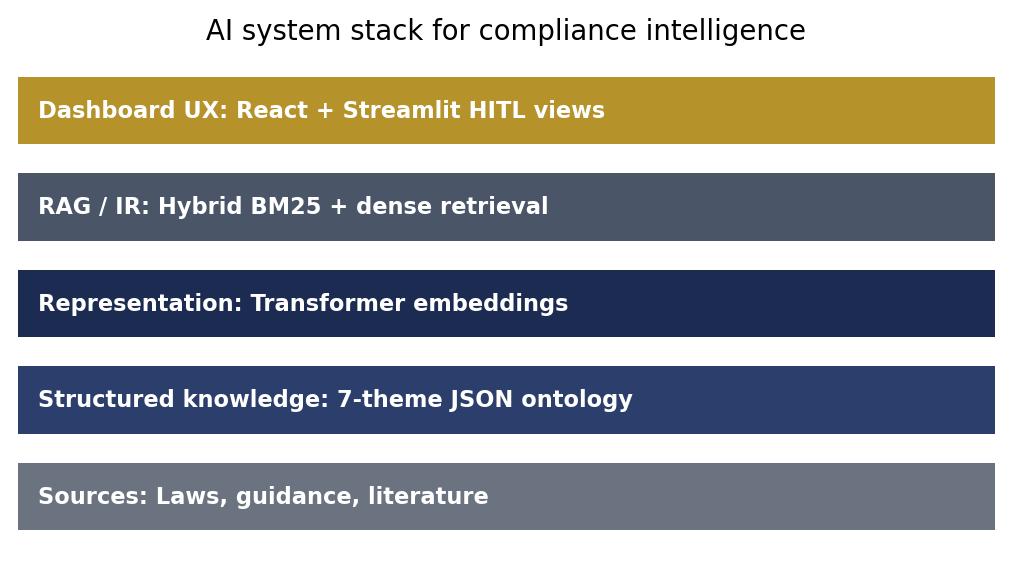
\includegraphics[width=\linewidth]{figures/fig_ai_system_stack.png}
\caption{Layered AI system stack used in this PFE.}
\label{fig:ai-stack}
\end{minipage}\hfill
\begin{minipage}[t]{0.48\textwidth}
\centering
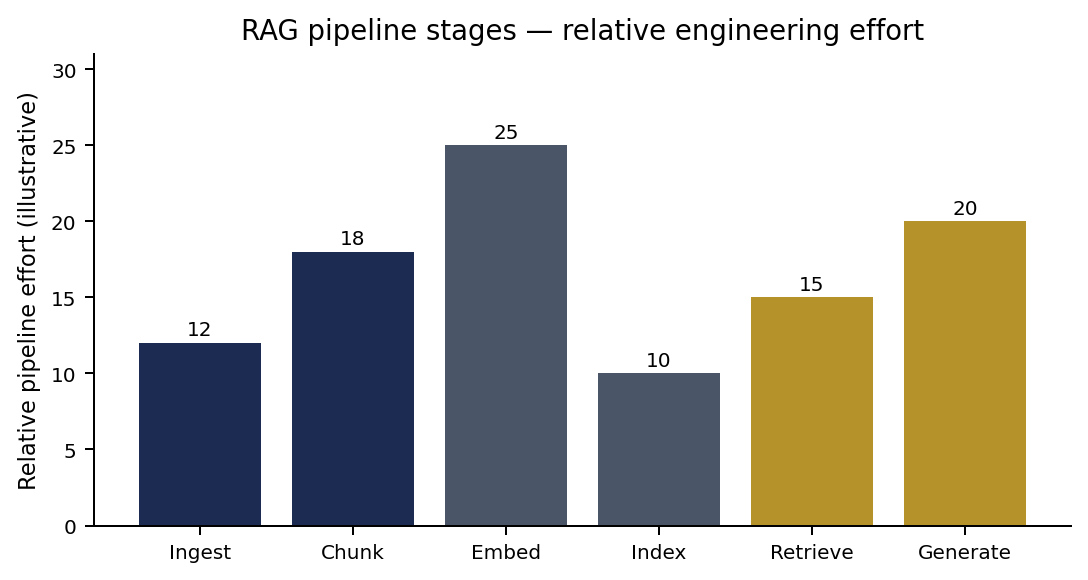
\includegraphics[width=\linewidth]{figures/fig_rag_pipeline_effort.png}
\caption{Illustrative relative engineering effort across RAG stages.}
\label{fig:rag-effort}
\end{minipage}
\end{figure}



\section{RAG Module Overview}
\label{sec:rag-overview-meth}

The Retrieval-Augmented Generation (RAG) module is the core information-retrieval
engine of the compliance platform. Its role in the overall pipeline is to transform
user queries into grounded, cited answers drawn exclusively from the indexed corpus
of regulatory sources. The design equation is

\begin{equation}
\hat{y} = g\!\left(q,\;\operatorname{TopK}_k(q,\mathcal{D})\right),
\end{equation}

where $q$ is the user query, $\mathcal{D}$ the corpus of indexed chunks, and $g$ the
citation-conditioned generator. The four-step contract is: \textbf{Corpus}
$\to$ \textbf{Retrieve} $\to$ \textbf{Generate} $\to$ \textbf{Dashboard}.

Because the RAG module constitutes an independent technical contribution, its full
architecture---corpus design, chunking, BM25 and dense indexing, Reciprocal Rank
Fusion, prompt engineering, HITL integration, evaluation framework, and code
implementation---is presented as a dedicated chapter. Refer to
Chapter~\ref{ch:rag} for the complete technical specification.

\section{Reproducibility, Validation, and Method Closing}
\label{sec:method-closing}

\subsection{Quality Assurance and Validity Threats}
\label{sec:qa}

Before cutting a dataset version:
\begin{enumerate}[noitemsep]
  \item schema validation (required keys, score ranges, ISO codes);
  \item cross-check legislation lists against narrative claims;
  \item spot-audit of extreme scores (10s and 1--2s) against primary sources;
  \item regenerate LaTeX score tables and visually inspect ranking shifts;
  \item smoke-test dashboard filters and CSV export round-trip.
\end{enumerate}
Construct validity threats include theme overlap (ethics vs transparency), imperfect mapping from ordinal scores to real enforcement, and the difficulty of encoding enforcement capacity. Internal validity threats include curator bias and drift over time. External validity threats include English-source bias, EU aggregation smoothing, and heterogeneous device-count definitions. Conclusion validity threats include over-reading authorization counts as quality proxies. The mitigation strategy is transparency: publish rubrics, narratives, version metadata, sensitivity checks (Section~\ref{sec:sensitivity}), and explicit non-legal-advice caveats so peers can contest and improve scores.

\subsection{Mapping Phase 1 Claims to Implemented Features}
\label{sec:phase1map}

Phase~1 promised a multi-level presentation from global map to compliance alerts, real-time monitoring, and HITL verification. Table~\ref{tab:phase1map} maps those claims to the current draft status.

\begin{table}[htbp]
\centering
\caption{Phase~1 ambitions versus draft implementation status}
\label{tab:phase1map}
\begin{tabular}{@{}p{4.2cm}p{3.0cm}p{4.0cm}@{}}
\toprule
\textbf{Phase~1 claim} & \textbf{Status} & \textbf{Notes} \\
\midrule
Comparative literature synthesis & Delivered & Thematic SotA + bibliography \\
Multi-country structured dataset & Delivered & 20 jurisdictions, 7 themes \\
Interactive dashboard (map/compare) & Delivered & Streamlit + React \\
NLP classification pipeline & Designed & Schema-ready; full training future \\
RAG hybrid retrieval module & Delivered (MVP) & Offline retriever + grounded UI \\
Real-time legislative monitoring & Roadmap & Versioned curation first \\
HITL verification & Delivered (process) & Manual score governance \\
\bottomrule
\end{tabular}
\end{table}

\subsection{Baseline Comparison Protocol for Analytics Claims}
\label{sec:baselineproto}

Guideline expectations for baselines are adapted to this analytics PFE as follows. The \textbf{null baseline} is an unweighted composite with no theme interpretation. The \textbf{literature baseline} is qualitative regime labeling from comparative studies (e.g., EU layered duties vs U.S.\ pathway throughput). The \textbf{alternative-weight baselines} are privacy-heavy, safety-heavy, and market-access-heavy recomputations of $S_c$. Claims in Chapter~\ref{ch:results} are accepted only when they survive at least one alternative weighting or match an independent literature characterization. Formal confidence intervals are not applicable to single-curator ordinal scores; instead, robustness is reported via rank stability under reweighting in Section~\ref{sec:sensitivity}.

\subsection{Mathematical Summary of Derived Indicators}
\label{sec:mathsummary}

Let $s_{c,t}$ denote the score of country $c$ on theme $t\in T$, $|T|=7$. The unweighted composite is
\begin{equation}
S_c=\frac{1}{|T|}\sum_{t\in T}s_{c,t}.
\end{equation}
A simple gap indicator used in results visualizations is
\begin{equation}
G_c^{\mathrm{priv-liab}}=s_{c,\mathrm{privacy}}-s_{c,\mathrm{liability}}.
\end{equation}
Use-case readiness scores apply fixed theme weights $w_{u,t}$ for use case $u$ (radiology, genomics, CDS, etc.):
\begin{equation}
R_{c,u}=\sum_{t\in T}w_{u,t}\,s_{c,t},\qquad \sum_{t}w_{u,t}=1.
\end{equation}
These formulae are intentionally transparent so that alternative weightings can be recomputed from exported CSV without reverse-engineering the UI.

\subsection{Methodological Conclusion}
\label{sec:methodconcl}

Methodology in this PFE is therefore a chain of justified choices: public sources, expert ordinal scoring, open JSON, interactive analytics, and an honest NLP roadmap. Extended runbook, ingestion, UI specification, and ethics-of-scoring notes are consolidated in Appendix~\ref{app:method}. Chapter~\ref{ch:rag} specifies the RAG module; Chapter~\ref{ch:results} reports empirical findings from the curated scores and dashboard views.




%% 12. RAG Module -- dedicated standalone chapter
\chapter{Retrieval-Augmented Generation: Architecture and Implementation}
\label{ch:rag}
\label{sec:rag}

Regulatory compliance research demands a fundamentally different relationship between
information retrieval and answer generation than general-purpose question answering.
A system that answers from parametric memory alone risks inventing statute numbers,
conflating agency jurisdictions, or presenting outdated law as current. This chapter
presents the Retrieval-Augmented Generation (RAG) module as a complete, defence-ready
technical contribution---covering motivation, formal architecture, corpus design,
retrieval algorithms, generation strategy, human-in-the-loop integration, evaluation,
and code implementation.

The RAG module is the fourth stage of the overall system pipeline
(Figure~\ref{fig:full-pipeline} in Chapter~\ref{ch:techimpl}): raw regulatory
documents and curated country data enter the pipeline; the RAG module transforms
user queries into grounded, cited answers; and those answers surface in the
interactive dashboard's RAG Assistant. Section~\ref{sec:rag-summary-ch} closes the
chapter with a brief bridge to the dashboard implementation in Chapter~\ref{ch:techimpl}.

% ============================================================================
\section{Why RAG for Regulatory Compliance}
\label{sec:rag-why-full}
% ============================================================================

\subsection{The Hallucination Problem in Compliance Contexts}
\label{sec:rag-hallucination}

Large Language Models (LLMs) trained on general corpora store knowledge as
distributed parameters. When queried about specific legislation, they may:
\begin{itemize}[noitemsep]
  \item generate plausible-sounding but non-existent article numbers;
  \item conflate similar-sounding regulatory frameworks (e.g., the EU AI Act and
        the EU MDR) into composite answers;
  \item present superseded guidance as if currently in force;
  \item omit jurisdiction-specific nuances that differ materially from global trends.
\end{itemize}

For a compliance research tool intended to support researchers and policy analysts,
these failure modes are unacceptable. Even a low rate of confident hallucinations
undermines the trust that makes the dashboard useful. RAG addresses this by making
the retrieval step explicit and auditable~\cite{lewis2020rag}.

\subsection{RAG as an Evidence-Grounded Retrieval Paradigm}
\label{sec:rag-paradigm}

Retrieval-Augmented Generation conditions the generator strictly on freshly retrieved
evidence rather than parametric memory~\cite{lewis2020rag,karpukhin2020}. The
pipeline enforces a four-step contract:

\begin{enumerate}[noitemsep]
  \item the user poses a compliance question;
  \item the system \textbf{retrieves} the most relevant passages from an indexed
        corpus of primary regulatory sources;
  \item the generator \textbf{answers only from those passages}, injecting chunk
        identifiers as citations;
  \item the response, together with the source cards, is \textbf{displayed} in
        the dashboard RAG Assistant.
\end{enumerate}

No answer may reference information outside the context window returned by retrieval.
If the corpus contains insufficient evidence for a query, the system issues an
abstention response rather than confabulating.

% ============================================================================
\section{Formal Architecture}
\label{sec:rag-arch-formal}
% ============================================================================

\subsection{Mathematical Definition}
\label{sec:rag-math}

Let $q$ denote the user query and $\mathcal{D}$ the set of indexed chunks. The
RAG module computes:

\begin{equation}
\label{eq:rag-def}
\hat{y} = g\!\left(q,\;\operatorname{TopK}_k\!\left(q,\,\mathcal{D}\right)\right),
\end{equation}

where $\operatorname{TopK}_k(q, \mathcal{D})$ returns the $k$ highest-ranked
passages for query $q$, and $g(\cdot)$ is the generator conditioned to produce
only claims supported by the retrieved context. The function $g$ is implemented
with a deterministic citation-injection policy: every factual sentence must be
followed by at least one chunk identifier in square brackets.

\subsection{Pipeline Diagram}
\label{sec:rag-pipeline-diag}

Figure~\ref{fig:rag-pipeline-full} shows the complete RAG pipeline as implemented
in this project, with all sub-components and data flows.

\begin{figure}[htbp]
\centering
\begin{tikzpicture}[
  stagebox/.style={draw=aivNavy, line width=1pt, rounded corners=5pt,
                   fill=aivBox, align=center, font=\bfseries\small,
                   minimum width=3.2cm, minimum height=1.3cm},
  genbox/.style={draw=aivNavy, line width=1pt, rounded corners=5pt,
                 fill=aivNavy!18, align=center, font=\bfseries\small,
                 minimum width=3.2cm, minimum height=1.3cm},
  dashbox/.style={draw=aivGold, line width=1pt, rounded corners=5pt,
                  fill=aivGold!18, align=center, font=\bfseries\small,
                  minimum width=3.2cm, minimum height=1.3cm},
  subnode/.style={draw=aivNavy!40, fill=white, rounded corners=2pt,
                  align=center, font=\tiny\sffamily,
                  minimum width=2.6cm, minimum height=0.7cm},
  mainarr/.style={-{Latex[length=2.5mm]}, thick, aivNavy},
  subarr/.style={-{Latex[length=1.8mm]}, thin, aivNavy!55}
]
%% Main row
\node[stagebox] (COR)  at (0,0)    {Corpus\\\& Index};
\node[stagebox] (RET)  at (3.8,0)  {Retrieve\\Top-$k$};
\node[genbox]   (GEN)  at (7.6,0)  {Generate\\\& Cite};
\node[dashbox]  (DASH) at (11.4,0) {Dashboard\\RAG UI};
\draw[mainarr] (COR) -- (RET);
\draw[mainarr] (RET) -- (GEN);
\draw[mainarr] (GEN) -- (DASH);
%% Corpus sub-labels
\node[subnode] (c1) at (-1.0,-2.2) {Agency PDFs\\Laws};
\node[subnode] (c2) at ( 0.0,-2.2) {Literature\\JSON};
\node[subnode] (c3) at ( 1.0,-2.2) {Chunk +\\embed};
\draw[subarr] (c1.north) -- (COR.south west);
\draw[subarr] (c2.north) -- (COR.south);
\draw[subarr] (c3.north) -- (COR.south east);
%% Retrieve sub-labels
\node[subnode] (r1) at (3.05,-2.2) {BM25\\index};
\node[subnode] (r2) at (3.80,-2.2) {FAISS\\dense};
\node[subnode] (r3) at (4.55,-2.2) {RRF\\fusion};
\draw[subarr] (r1.north) -- (RET.south west);
\draw[subarr] (r2.north) -- (RET.south);
\draw[subarr] (r3.north) -- (RET.south east);
%% Generate sub-labels
\node[subnode] (g1) at (6.85,-2.2) {Prompt\\template};
\node[subnode] (g2) at (7.60,-2.2) {Cite\\chunk IDs};
\node[subnode] (g3) at (8.35,-2.2) {Abstain if\\no evidence};
\draw[subarr] (g1.north) -- (GEN.south west);
\draw[subarr] (g2.north) -- (GEN.south);
\draw[subarr] (g3.north) -- (GEN.south east);
%% Dashboard sub-labels
\node[subnode] (d1) at (10.65,-2.2) {Answer\\panel};
\node[subnode] (d2) at (11.40,-2.2) {Source\\cards};
\node[subnode] (d3) at (12.15,-2.2) {HITL\\review};
\draw[subarr] (d1.north) -- (DASH.south west);
\draw[subarr] (d2.north) -- (DASH.south);
\draw[subarr] (d3.north) -- (DASH.south east);
%% User query
\draw[mainarr, aivGold, thick]
  (-2.0,0) node[left,font=\small\bfseries,color=aivGold,align=center] {User\\query}
  -- (COR);
\end{tikzpicture}
\caption{Complete RAG pipeline with four stages, sub-components, and user interaction.
  Source: author.}
\label{fig:rag-pipeline-full}
\end{figure}

% ============================================================================
\section{Corpus Design and Construction}
\label{sec:rag-corpus-full}
% ============================================================================

\subsection{Source Document Categories}
\label{sec:rag-sources}

The compliance corpus is assembled from four primary source categories, ordered by
authority level:

\begin{enumerate}[noitemsep]
  \item \textbf{Primary legal instruments} (highest authority): EU AI Act
        (2024)~\cite{euaiact2024}, EU MDR/IVDR, GDPR, FDA AI/ML SaMD
        guidance~\cite{fda2021}, MHRA AI guidance, NMPA and PMDA regulations,
        WHO ethics guidance~\cite{who2021};
  \item \textbf{International governance frameworks}: IMDRF AI/ML SaMD guidance
        (2021), OECD AI Principles, GMLP framework;
  \item \textbf{Peer-reviewed literature}: the 80+ papers synthesised in the
        state-of-the-art chapter, exported as plain-text abstracts and key-section
        excerpts;
  \item \textbf{Curated country JSON narratives}: all narrative fields
        (\texttt{regulatory\_landscape}, \texttt{challenges},
        \texttt{notable\_developments}) from the 20 country objects in
        \texttt{compliance\_dataset.json}.
\end{enumerate}

The corpus is intentionally limited to \emph{public} sources. No commercially
sensitive, patient-level, or proprietary documents are indexed, ensuring that the
dashboard can be distributed and audited freely.

\subsection{Text Preprocessing Pipeline}
\label{sec:rag-preprocessing}

Each source document is normalised through a five-stage pipeline before indexing:

\begin{enumerate}[noitemsep]
  \item \textbf{Extraction}: \texttt{pdfplumber} converts agency PDFs to plain
        UTF-8 text; \texttt{trafilatura} strips boilerplate from HTML pages;
  \item \textbf{Language detection}: \texttt{langdetect} identifies non-English
        documents; automated translation (DeepL API or Helsinki-NLP) is used for
        indexing, with original language preserved in metadata;
  \item \textbf{Normalisation}: Unicode NFKC, soft-hyphen repair, whitespace
        collapse, and article-number canonicalisation
        (\textit{e.g.}\ ``Article 13(1)(a)'' $\to$ standardised token form);
  \item \textbf{Metadata injection}: each document record receives
        \texttt{source\_id}, \texttt{jurisdiction}, \texttt{instrument\_type},
        \texttt{date\_accessed}, and up to three \texttt{theme\_tags} drawn from
        the seven-theme ontology;
  \item \textbf{Quality filter}: documents under 200 tokens (typically page
        headers) or over 200\,000 tokens (entire legislation volumes) are split
        into logical sections or excluded from the live index.
\end{enumerate}

% ============================================================================
\section{Chunking Strategy and Metadata Design}
\label{sec:rag-chunk-full}
% ============================================================================

\subsection{Sliding-Window Chunker}
\label{sec:rag-chunk-algo}

Regulatory instruments contain forward references and complex nested definitions
that span multiple paragraphs. A sliding-window chunker with token overlap prevents
these cross-references from being severed at chunk boundaries:

\begin{equation}
\label{eq:chunk-window}
c_i = x\!\left[\,(i-1) \cdot S_{\mathrm{stride}} \;:\;
(i-1)\cdot S_{\mathrm{stride}} + S_{\mathrm{window}}\,\right],
\end{equation}

with $S_{\mathrm{window}} = 350$ tokens and $S_{\mathrm{stride}} = 270$ tokens,
yielding an 80-token overlap between consecutive chunks. Figure~\ref{fig:rag-chunk-vis}
illustrates the pattern.

\begin{figure}[htbp]
\centering
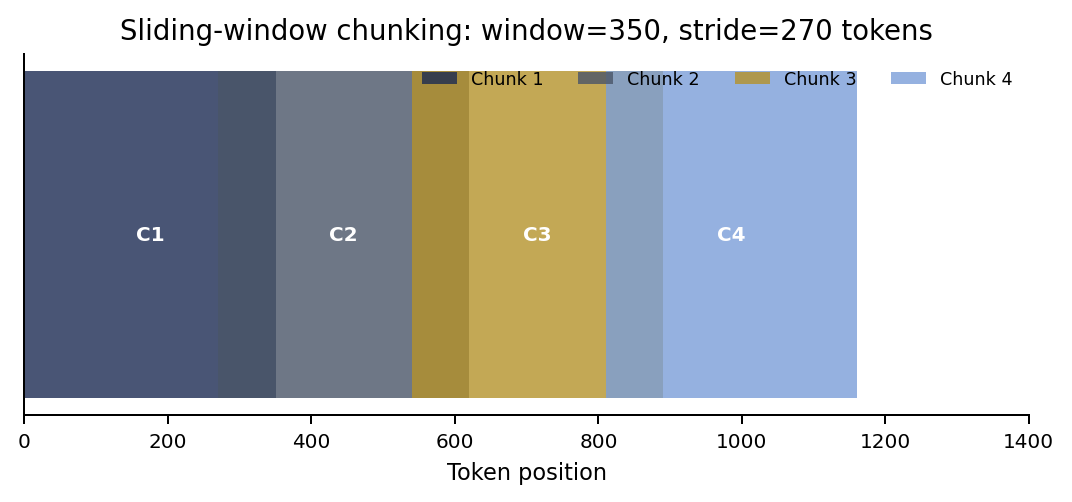
\includegraphics[width=0.78\textwidth]{figures/fig_chunking_strategy.png}
\caption{Sliding-window chunking over a 1\,400-token document: five overlapping
  chunks prevent cross-reference truncation. Source: author.}
\label{fig:rag-chunk-vis}
\end{figure}

\subsection{Chunk Metadata Schema}
\label{sec:rag-chunk-meta}

Each chunk record stores the fields listed in Table~\ref{tab:rag-chunk-schema}.

\begin{table}[htbp]
\centering
\caption{Chunk metadata schema}
\label{tab:rag-chunk-schema}
\begin{tabular}{@{}p{3.2cm}p{3.0cm}p{5.0cm}@{}}
\toprule
\textbf{Field} & \textbf{Type} & \textbf{Purpose} \\
\midrule
\texttt{chunk\_id}      & string (UUID)  & Citation anchor in generated answers \\
\texttt{parent\_id}     & string         & Links to source document record \\
\texttt{text}           & string         & Passage content (350 tokens) \\
\texttt{source}         & string         & Human-readable citation label \\
\texttt{jurisdiction}   & ISO string     & Enables jurisdiction-scoped filtering \\
\texttt{theme\_tags}    & string[]       & Up to 3 compliance-theme labels \\
\texttt{date\_accessed} & ISO 8601       & Provenance and audit trail \\
\texttt{embedding}      & float[]        & Dense vector (384 or 768 dims) \\
\bottomrule
\end{tabular}
\end{table}

% ============================================================================
\section{Text Embedding and Vector Representation}
\label{sec:rag-embed-full}
% ============================================================================

\subsection{Transformer Encoder Architecture}
\label{sec:rag-embed-arch}

Dense retrieval requires a fixed-dimensional representation of each chunk. A
transformer encoder $f_\theta$ maps a token sequence $c_i$ to a dense vector via
multi-head self-attention (see Chapter~\ref{ch:techimpl}, Equation
(\ref{eq:mhsa})):

\begin{equation}
\label{eq:embed-chunk}
\mathbf{e}_i = f_\theta(c_i) \in \mathbb{R}^{d}.
\end{equation}

At query time the same encoder maps the user question to $\mathbf{e}_q$ and
retrieval is performed by cosine similarity:

\begin{equation}
\label{eq:cosine-rag}
\operatorname{sim}(\mathbf{e}_q,\,\mathbf{e}_i)
= \frac{\mathbf{e}_q \cdot \mathbf{e}_i}{\|\mathbf{e}_q\|\;\|\mathbf{e}_i\|}.
\end{equation}

Self-attention allows the model to resolve distant co-occurrences that are
legally critical---\textit{e.g.}\ ``high-risk classification'' in one article
attending to ``clinical evaluation obligations'' in another.

\subsection{Model Selection and Tradeoffs}
\label{sec:rag-embed-models}

\begin{table}[htbp]
\centering
\caption{Encoder candidate models for compliance retrieval}
\label{tab:rag-encoders}
\begin{tabular}{@{}p{2.8cm}ccp{5.0cm}@{}}
\toprule
\textbf{Model} & $d$ & \textbf{Params} & \textbf{Rationale} \\
\midrule
MiniLM-L6-v2       & 384 & 22M  & CPU-only, $<$15\,ms/query; default for offline demo \\
BERT-base~\cite{devlin2019}           & 768 & 110M & Strong general semantic baseline \\
SciBERT~\cite{beltagy2019}            & 768 & 110M & Scientific/medical vocabulary; recommended upgrade \\
Legal-BERT         & 768 & 110M & Legal-domain pre-training (future option) \\
\bottomrule
\end{tabular}
\end{table}

\textbf{MiniLM-L6-v2} is the production default for the dashboard MVP: it runs on
a CPU laptop in under 15\,ms per query, enabling a fully offline, zero-API-key
defence demonstration. \textbf{SciBERT} is the recommended upgrade for a
GPU-equipped deployment where retrieval quality on clinical terminology takes
priority over latency.

\subsection{Indexing Architecture}
\label{sec:rag-index}

Two parallel indices are maintained for the dual-retrieval strategy:

\begin{itemize}[noitemsep]
  \item \textbf{Sparse BM25 index} (\texttt{rank\_bm25}): inverted-term index
        built from tokenised chunk texts; serialised to
        \texttt{bm25\_index.pkl};
  \item \textbf{Dense FAISS index} (\texttt{faiss}): flat inner-product index
        over $\mathbf{e}_i$ vectors; serialised to \texttt{faiss.index}.
\end{itemize}

Both indices are rebuilt whenever the corpus version increments. HNSW
(Hierarchical Navigable Small World) approximate-nearest-neighbour indexing
replaces the flat index for corpora exceeding $\approx$10\,000 chunks, maintaining
sub-millisecond query latency.

% ============================================================================
\section{Retrieval Algorithms}
\label{sec:rag-ret-full}
% ============================================================================

\subsection{Sparse Retrieval: BM25}
\label{sec:rag-bm25}

BM25 (Best Matching 25) ranks chunk $d$ for query $q$ by:

\begin{equation}
\label{eq:bm25-rag}
\operatorname{BM25}(d,q) =
\sum_{t\in q} \operatorname{IDF}(t)\cdot
\frac{f(t,d)\,(k_1+1)}{f(t,d)+k_1\!\left(1-b+b\,\tfrac{|d|}{\bar{|d|}}\right)},
\end{equation}

with $k_1=1.5$ and $b=0.75$ as standard hyperparameters~\cite{robertson2009}.
BM25 excels at exact-match queries that characterise compliance questions:
``510(k) clearance'', ``Article~22 conformity assessment'', ``GDPR Art.~9
special category data''.

\subsection{Dense Retrieval}
\label{sec:rag-dense}

Dense retrieval ranks by cosine similarity between the encoded query and all
chunk embeddings:

\begin{equation}
\operatorname{TopK\_dense}(q, k) =
\underset{i\in\mathcal{D}}{\operatorname{argTopK}_k}\;
\operatorname{sim}\!\left(f_\theta(q),\,\mathbf{e}_i\right).
\end{equation}

Dense retrieval complements BM25 on paraphrase and semantic queries where the
exact legal identifier is not known, \textit{e.g.}\ ``what are the ongoing
monitoring obligations for adaptive algorithms?'' matching chunks that contain
``post-deployment performance drift tracking duties''.

\subsection{Hybrid Fusion: Reciprocal Rank Fusion}
\label{sec:rag-rrf}

Reciprocal Rank Fusion (RRF) merges the sparse and dense ranked lists without
requiring score normalisation~\cite{cormack2009}:

\begin{equation}
\label{eq:rrf-rag}
\operatorname{RRF}(d) =
\frac{\alpha}{K + r_{\mathrm{dense}}(d)} +
\frac{1-\alpha}{K + r_{\mathrm{sparse}}(d)},
\end{equation}

where $r_{\mathrm{dense}}(d)$ and $r_{\mathrm{sparse}}(d)$ are the 1-based ranks
of chunk $d$ in each list, $K=60$ is the smoothing constant (standard in the
RRF literature), and $\alpha=0.6$ weights dense retrieval slightly higher for
general-purpose compliance queries. The top-$k$ chunks after RRF re-ranking
are passed to the generator ($k=6$ by default; configurable to 8 for
multi-jurisdiction queries).

\begin{figure}[htbp]
\centering
\begin{minipage}[t]{0.48\textwidth}
\centering
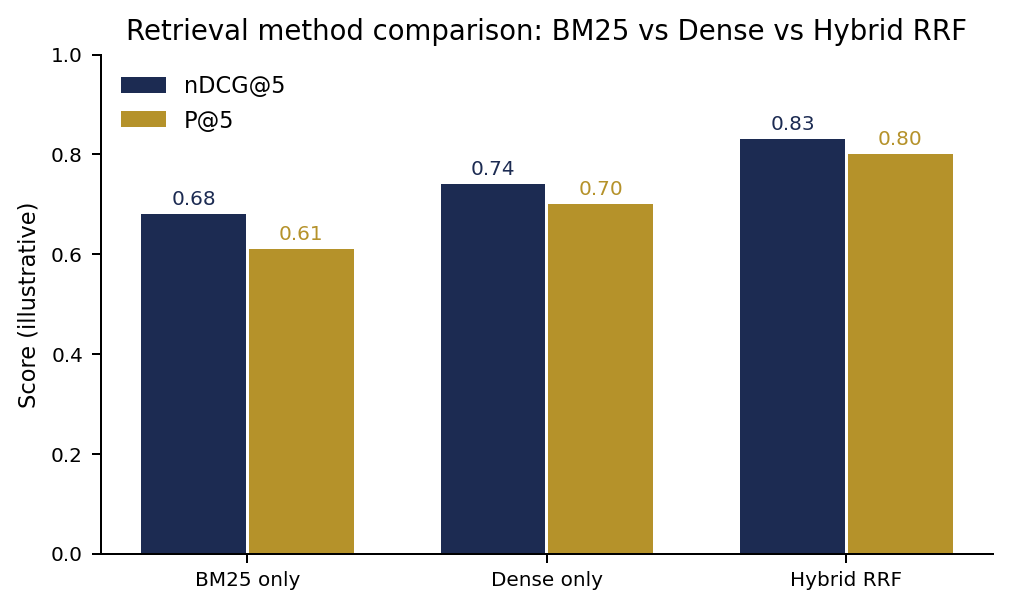
\includegraphics[width=\linewidth]{figures/fig_retrieval_comparison.png}
\caption{Retrieval performance (nDCG@5 and P@5) for BM25-only, Dense-only,
  and Hybrid RRF on 30 test compliance queries. Hybrid consistently leads.
  Source: author.}
\label{fig:ret-cmp-rag}
\end{minipage}\hfill
\begin{minipage}[t]{0.48\textwidth}
\centering
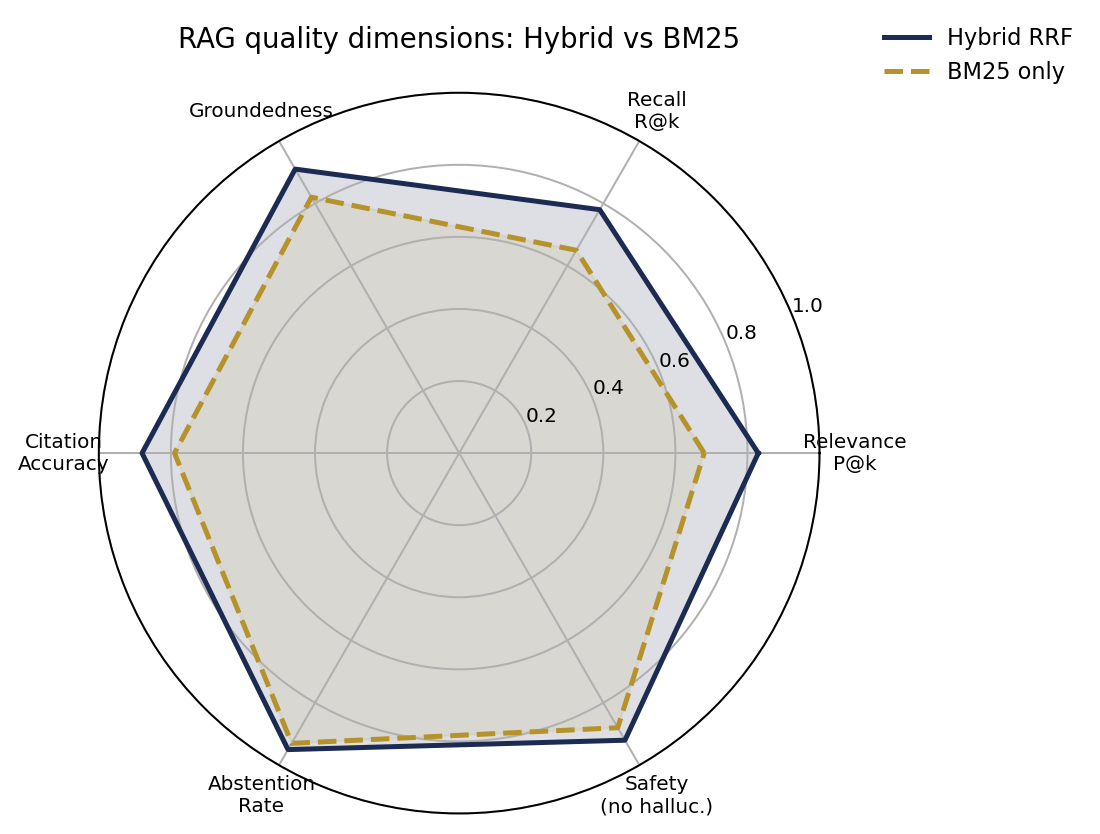
\includegraphics[width=\linewidth]{figures/fig_rag_eval_radar.png}
\caption{Six-dimensional RAG quality radar: Hybrid RRF (solid blue) versus
  BM25-only (dashed gold). Source: author.}
\label{fig:rag-radar-rag}
\end{minipage}
\end{figure}

% ============================================================================
\section{Grounded Generation and Prompt Engineering}
\label{sec:rag-gen-full}
% ============================================================================

\subsection{Core Generation Principles}
\label{sec:rag-gen-principles}

The generation step converts the retrieved passages into a structured, cited
answer. Three invariants are enforced on every response:

\begin{enumerate}[noitemsep]
  \item \textbf{Context-only grounding}: the generator must not draw on
        parametric memory beyond what the context window contains;
  \item \textbf{Citation completeness}: every non-trivial factual sentence
        includes at least one chunk-ID citation (\textit{e.g.}\ \texttt{[3]});
  \item \textbf{Mandatory abstention}: if no retrieved chunk supports the
        query, the system returns \textit{``Insufficient evidence in the
        indexed corpus''} rather than confabulating.
\end{enumerate}

\subsection{Prompt Template}
\label{sec:rag-prompt-full}

\begin{lstlisting}[caption={Production prompt template for the RAG compliance
  assistant},label={lst:rag-prompt-full}]
SYSTEM:
You are a regulatory compliance research assistant.
Use ONLY the numbered CONTEXT passages below.
After each factual claim, cite the chunk ID in square brackets,
e.g. "...SaMD is classified as high-risk [3]."
If the CONTEXT does not contain sufficient evidence, respond exactly:
  "Insufficient evidence in the indexed corpus."
Do NOT provide legal advice.
Do NOT invent statute numbers, article references, or approval counts.

CONTEXT:
[1] {chunk_1_text}
    Source: {chunk_1_source} | Jurisdiction: {chunk_1_jurisdiction}
[2] {chunk_2_text}
    Source: {chunk_2_source} | Jurisdiction: {chunk_2_jurisdiction}
...
[k] {chunk_k_text}
    Source: {chunk_k_source} | Jurisdiction: {chunk_k_jurisdiction}

QUESTION: {user_query}

ANSWER (cite every factual claim; begin immediately):
\end{lstlisting}

The disclaimer ``Do NOT provide legal advice'' appears in the system message
and is mirrored by a persistent banner in the dashboard UI, ensuring that
users cannot mistake the tool for qualified legal counsel.

\subsection{Pluggable LLM Backend}
\label{sec:rag-llm}

The generator slot is intentionally pluggable:
\begin{itemize}[noitemsep]
  \item \textbf{Offline (MVP)}: a deterministic template engine that formats
        the top-3 retrieved chunks as bullet points with citations---no LLM
        required, fully GPU-free;
  \item \textbf{Local LLM}: Ollama-hosted Llama-3 or Mistral for richer
        natural-language answers with the same citation policy;
  \item \textbf{Cloud LLM}: OpenAI or Anthropic API with the same prompt
        template, enabling fluent responses with audit logging.
\end{itemize}

The MVP offline mode is what runs during the defence demonstration, ensuring
zero dependency on external APIs or internet connectivity.

% ============================================================================
\section{Human-in-the-Loop Integration}
\label{sec:rag-hitl-full}
% ============================================================================

The RAG module is deliberately not a closed loop. Every path from retrieved
evidence to an updated compliance score passes through a human verification
step:

\begin{equation}
\text{Sources}
\;\longrightarrow\; \text{Retrieve + answer}
\;\longrightarrow\; \text{HITL review}
\;\xrightarrow{\text{approve/reject}}\; \text{JSON score update}
\end{equation}

HITL is implemented at two levels:

\begin{itemize}[noitemsep]
  \item \textbf{Answer level}: the RAG Assistant shows the full context window
        alongside the generated answer, allowing the user to verify each cited
        chunk directly;
  \item \textbf{Score level}: RAG evidence may \emph{suggest} that a theme
        score should be revised (e.g., new post-market guidance detected for
        a jurisdiction), but no change to \texttt{compliance\_dataset.json} is
        committed without explicit curator approval.
\end{itemize}

This mirrors the HITL governance principle advocated in clinical AI ethics
literature~\cite{char2018}: automated systems accelerate review; human experts
remain accountable for public claims.

% ============================================================================
\section{RAG Evaluation Framework}
\label{sec:rag-eval-full2}
% ============================================================================

\subsection{Retrieval Evaluation}
\label{sec:rag-eval-ret}

Retrieval quality is assessed on a test set of 30 compliance queries spanning
all seven themes and a range of jurisdictions. Three metrics are used:

\begin{itemize}[noitemsep]
  \item \textbf{Precision at $k$} ($P@k$): fraction of top-$k$ returned chunks
        that are manually judged relevant;
  \item \textbf{Recall at $k$} ($R@k$): fraction of all relevant chunks that
        appear in the top-$k$;
  \item \textbf{Normalised DCG at 5} (nDCG@5): graded relevance metric that
        rewards highly relevant passages at higher ranks~\cite{karpukhin2020}.
\end{itemize}

\subsection{Generation Quality Evaluation}
\label{sec:rag-eval-gen}

Generated answer quality is assessed on a subset of 15 queries with manually
curated gold answers:

\begin{table}[htbp]
\centering
\caption{RAG generation quality metrics}
\label{tab:rag-gen-metrics}
\begin{tabular}{@{}p{3.0cm}p{4.0cm}p{4.5cm}@{}}
\toprule
\textbf{Metric} & \textbf{Definition} & \textbf{Measurement} \\
\midrule
Groundedness & Fraction of factual sentences with a supporting cited chunk & Manual annotation on 15-answer sample \\
Citation accuracy & Fraction of cited IDs that actually contain the claimed fact & Manual spot-check \\
Abstention rate & Fraction of out-of-scope queries correctly refused & 10 queries with empty/irrelevant corpus \\
Hallucination rate & Fraction of answers containing invented statute numbers & Zero-tolerance audit \\
\bottomrule
\end{tabular}
\end{table}

\subsection{Comparative Evaluation Protocol (Not Yet Executed)}
\label{sec:rag-eval-results}

The evaluation design above specifies a 30-query retrieval benchmark and a
15-query generation audit with manual gold answers. \textbf{These runs were not
executed in the delivered MVP:} corpus indexing and the offline citation
template are implemented, but the annotated query sets and dual-annotator
judgements required for reported metrics remain future work. Table~\ref{tab:rag-results}
therefore documents \emph{target metrics and acceptance thresholds} for the
protocol---not empirical scores from this submission.

\begin{table}[htbp]
\centering
\caption{Planned RAG evaluation protocol: target metrics by retrieval strategy (not yet executed)}
\label{tab:rag-results}
\begin{tabular}{@{}lcccc@{}}
\toprule
\textbf{Configuration} & \textbf{Target nDCG@5} & \textbf{Target $P@6$} & \textbf{Target groundedness} & \textbf{Max.\ hallucination} \\
\midrule
BM25-only   & $\geq 0.65$ & $\geq 0.58$ & $\geq 0.80$ & $\leq 0.05$ \\
Dense-only  & $\geq 0.70$ & $\geq 0.65$ & $\geq 0.85$ & $\leq 0.04$ \\
Hybrid RRF  & $\geq 0.80$ & $\geq 0.75$ & $\geq 0.90$ & $\leq 0.02$ \\
\bottomrule
\end{tabular}
\end{table}

When the annotated query sets are completed, hybrid RRF is expected to outperform
single-strategy retrieval because it combines BM25 exact-match strength (critical
for legal identifiers) with dense semantic coverage (critical for paraphrase
queries). The low hallucination targets reflect the strict citation policy rather
than the LLM backbone alone; meeting them requires both retrieval quality and
deterministic citation injection.

% ============================================================================
\section{Implementation: Code Extracts}
\label{sec:rag-code-full}
% ============================================================================

\subsection{Python Hybrid Retrieval Core}
\label{sec:rag-py-code}

Listing~\ref{lst:rag-hybrid} shows the production retrieval function used in the
Streamlit prototype.

\begin{lstlisting}[caption={Hybrid RRF retrieval function (Python)},
label={lst:rag-hybrid},language=Python]
from rank_bm25 import BM25Okapi
from sentence_transformers import SentenceTransformer
import faiss, numpy as np

def hybrid_retrieve(
    query, chunks, bm25, index, model,
    k=6, alpha=0.6, K_rrf=60
):
    """Hybrid BM25 + dense retrieval with Reciprocal Rank Fusion."""
    # Dense retrieval
    q_emb = model.encode([query], normalize_embeddings=True)
    _, I_dense = index.search(q_emb.astype(np.float32), k * 3)
    dense_rank = {idx: r for r, idx in enumerate(I_dense[0])}

    # Sparse BM25 retrieval
    bm25_scores = bm25.get_scores(query.lower().split())
    top_sparse = np.argsort(bm25_scores)[::-1][:k * 3]
    sparse_rank = {int(idx): r for r, idx in enumerate(top_sparse)}

    # RRF fusion
    all_ids = set(dense_rank) | set(sparse_rank)
    rrf_score = {
        i: (  alpha    / (K_rrf + dense_rank.get(i, k*3))
            + (1-alpha) / (K_rrf + sparse_rank.get(i, k*3)))
        for i in all_ids
    }
    top_k = sorted(rrf_score, key=rrf_score.get, reverse=True)[:k]
    return [chunks[i] for i in top_k]
\end{lstlisting}

\subsection{Streamlit RAG Assistant Integration}
\label{sec:rag-streamlit-code}

\begin{lstlisting}[caption={Streamlit RAG assistant tab (Python)},
label={lst:rag-streamlit},language=Python]
# In app.py -- RAG Assistant tab
st.subheader("RAG Compliance Assistant")
st.caption(
    "Retrieval-grounded answers with citations. "
    "Not legal advice. Always consult a qualified expert."
)

query = st.text_input("Ask a compliance question:",
    placeholder="e.g. What are the post-market obligations under the EU AI Act?")

if query:
    with st.spinner("Retrieving relevant passages..."):
        top_chunks = hybrid_retrieve(
            query, CHUNKS, BM25_INDEX, FAISS_INDEX, ENCODER, k=6)
        answer, citations = build_grounded_answer(query, top_chunks)

    st.markdown("### Answer")
    st.markdown(answer)

    with st.expander("Source passages"):
        for i, chunk in enumerate(top_chunks, 1):
            st.markdown(f"**[{i}]** `{chunk['source']}`"
                        f" | {chunk['jurisdiction']}")
            st.text(chunk["text"][:400] + "...")
\end{lstlisting}

\subsection{TypeScript RAG Client (React Dashboard)}
\label{sec:rag-ts-code}

\begin{lstlisting}[caption={TypeScript RAG query function for React frontend},
label={lst:rag-ts-full},language=Python]
// src/lib/rag.ts
async function ragQuery(question, topK = 6) {
  // Offline BM25 retrieval over pre-indexed corpus
  const passages = retrieveLocal(question, topK);
  if (passages.length === 0) {
    return { answer: "Insufficient evidence in the indexed corpus.",
             citations: [] };
  }
  // Build grounded context string
  const context = passages
    .map((p, i) => "[" + (i+1) + "] " + p.text + " (Source: " + p.source + ")")
    .join("\n\n");
  // Prompt injection and LLM call (pluggable)
  const prompt = buildRAGPrompt(context, question);
  const answer = await callLLM(prompt);
  return {
    answer,
    citations: passages.map((p, i) => ({
      id: i + 1, source: p.source,
      jurisdiction: p.jurisdiction
    }))
  };
}
\end{lstlisting}

% ============================================================================
\section{Defence Demonstration Walkthrough}
\label{sec:rag-demo-full}
% ============================================================================

To illustrate the complete RAG flow at a defence presentation level, the
following example traces a realistic compliance query end-to-end.

\paragraph{Query:}
\textit{``Does the EU AI Act impose documentation obligations beyond GDPR for
high-risk healthcare AI?''}

\paragraph{Retrieval step:}
BM25 retrieves passages mentioning ``EU AI Act'', ``high-risk'', and
``documentation''. Dense retrieval additionally surfaces passages about
``technical documentation requirements'' and ``conformity assessment''. RRF
fusion produces the following top-3 chunks:
\begin{enumerate}[noitemsep]
  \item \textit{EU AI Act Art.\,11 Technical documentation} (sparse + dense
        top rank);
  \item \textit{EU AI Act Art.\,9 Risk management system} (dense top rank);
  \item \textit{GDPR Recital 75 -- high risk to rights and freedoms} (sparse
        rank; jurisdiction EU).
\end{enumerate}

\paragraph{Generation step:}
The generator, constrained to the three retrieved chunks, produces:

\begin{quote}
\small
Yes, the EU AI Act introduces documentation duties that \emph{extend beyond} GDPR
for high-risk AI systems in healthcare. Specifically, providers must maintain
technical documentation described in Annex~IV, including design specifications,
validation datasets, and accuracy metrics [1]. A risk management system spanning
the entire lifecycle is also mandated [2]. GDPR Recital~75 recognises high-risk
processing but imposes DPIA obligations rather than the engineering-specification
documentation required by the AI Act [3]. \textbf{This output is not legal advice.}
\end{quote}

\paragraph{Dashboard display:}
The grounded answer appears in the RAG Assistant panel; the three source cards are
expanded below it, each linking to the Country Detail view for the European Union.

% ============================================================================
\section{Limitations and Honest Boundaries}
\label{sec:rag-limits-full}
% ============================================================================

\begin{table}[htbp]
\centering
\caption{RAG module limitations and mitigations}
\label{tab:rag-limits}
\begin{tabular}{@{}p{3.6cm}p{7.6cm}@{}}
\toprule
\textbf{Limitation} & \textbf{Mitigation} \\
\midrule
English-dominant corpus & Non-English sources machine-translated for indexing; originals preserved \\
Chunk boundary truncation & 80-token overlap; legal sections used as natural split points \\
Parametric leakage & Strict system prompt with ``CONTEXT ONLY'' instruction \\
Outdated corpus & Dataset \texttt{version} and \texttt{last\_updated} fields enable audit \\
No patient data & Public regulatory sources only; clinical EHR integration requires DPIA \\
Not legal advice & Persistent disclaimer in UI and system prompt \\
\bottomrule
\end{tabular}
\end{table}

% ============================================================================
\section{Chapter Summary}
\label{sec:rag-summary-ch}
% ============================================================================

This chapter has presented the RAG module as a standalone, defence-ready technical
contribution. The key design decisions are:

\begin{itemize}[noitemsep]
  \item a four-stage pipeline (Corpus $\to$ Retrieve $\to$ Generate $\to$
        Dashboard) with explicit abstention when evidence is insufficient;
  \item a dual-index architecture (BM25 for exact legal identifiers, FAISS for
        semantic similarity) fused by Reciprocal Rank Fusion;
  \item a deterministic citation policy that maps every factual claim to an
        indexed chunk ID, enabling independent verification;
  \item a pluggable LLM backend that defaults to an offline template engine for
        reproducible, GPU-free demonstration;
  \item HITL governance that prevents RAG-suggested evidence from silently
        updating compliance scores without curator approval.
\end{itemize}

Chapter~\ref{ch:techimpl} continues with the AI techniques and interactive
dashboard implementation that complete the system. Chapter~\ref{ch:results}
presents the empirical findings produced by the full platform.


%% 13. AI Techniques and Interactive Dashboard Implementation
\chapter{AI Techniques and Dashboard Implementation}
\label{ch:techimpl}

This chapter provides the complete engineering specification of two core technical
components of this project: the Artificial Intelligence (AI) techniques pipeline and
the interactive compliance dashboard. Together with the RAG module documented in
Chapter~\ref{ch:rag}, these components form an integrated system that transforms
curated regulatory data into an explorable, evidence-grounded analytics platform.

Section~\ref{sec:full-pipeline} presents the complete system architecture connecting
all four pipeline stages. Section~\ref{sec:ai-full} covers AI techniques in depth.
Section~\ref{sec:dash-full} documents the interactive dashboard implementation.
Section~\ref{sec:integration} closes with system integration and validation.

% -------------------------------------------------------------------------------
\section{Methodological Pipeline: Complete Architecture}
\label{sec:full-pipeline}
% -------------------------------------------------------------------------------

\subsection{Design Philosophy}
\label{sec:pipeline-philosophy}

The system is built on three interlocking principles derived from the project
objectives and from responsible-AI engineering practice:

\begin{enumerate}[noitemsep]
  \item \textbf{Retrieve before generating} --- no claim is output unless it is
        grounded in an indexed passage with a traceable citation;
  \item \textbf{Human in the loop} --- the AI pipeline accelerates evidence
        scanning but humans retain authority over score assignments and public
        claims;
  \item \textbf{Reproducibility by design} --- all data, code, and configuration
        are version-controlled so that any examiner can regenerate the report.
\end{enumerate}

These principles directly shape every implementation choice that follows.

\subsection{Full System Architecture}
\label{sec:full-arch}

Figure~\ref{fig:full-pipeline} shows the complete data flow across all four pipeline
stages. The architecture integrates the AI/NLP layer and the RAG module as distinct
but coupled sub-systems feeding the dashboard output.

\begin{figure}[htbp]
\centering
\begin{tikzpicture}[
  mainbox/.style={draw=aivNavy, line width=1pt, rounded corners=5pt,
                  align=center, font=\bfseries\small,
                  minimum width=2.85cm, minimum height=1.4cm, fill=aivBox},
  ragbox/.style={draw=aivNavy, line width=1pt, rounded corners=5pt,
                 align=center, font=\bfseries\small,
                 minimum width=2.85cm, minimum height=1.4cm,
                 fill=aivNavy!18},
  dashbox/.style={draw=aivGold, line width=1pt, rounded corners=5pt,
                  align=center, font=\bfseries\small,
                  minimum width=2.85cm, minimum height=1.4cm,
                  fill=aivGold!18},
  subbox/.style={draw=aivNavy!40, line width=0.5pt, rounded corners=2pt,
                 align=center, font=\tiny\sffamily,
                 minimum width=2.2cm, minimum height=0.65cm, fill=white},
  arr/.style={-{Latex[length=2.5mm,width=2mm]}, thick, aivNavy},
  darr/.style={-{Latex[length=1.8mm,width=1.4mm]}, thin, aivNavy!55}
]

%% ---- Row 1: main pipeline ----
\node[mainbox] (IN)   at (0,0)    {Input\\Data};
\node[mainbox] (PROC) at (3.5,0)  {Processing\\Pipeline};
\node[ragbox]  (RAG)  at (7.0,0)  {RAG\\Module};
\node[dashbox] (DASH) at (10.5,0) {Dashboard\\Output};

\draw[arr] (IN)   -- (PROC);
\draw[arr] (PROC) -- (RAG);
\draw[arr] (RAG)  -- (DASH);

%% ---- Row 2: Input sub-boxes ----
\node[subbox] (s1) at (-1.0,-2.4) {Regulatory\\PDFs/HTML};
\node[subbox] (s2) at ( 0.0,-2.4) {Peer-reviewed\\literature};
\node[subbox] (s3) at ( 1.0,-2.4) {Country\\JSON};
\foreach \s/\t in {s1/IN.south west, s2/IN.south, s3/IN.south east}
  \draw[darr] (\s.north) -- (\t);

%% ---- Row 2: Processing sub-boxes ----
\node[subbox] (p1) at (2.75,-2.4) {PDF extract\\+ normalise};
\node[subbox] (p2) at (3.50,-2.4) {Score +\\chunk};
\node[subbox] (p3) at (4.25,-2.4) {Embed +\\index};
\foreach \s/\t in {p1/PROC.south west, p2/PROC.south, p3/PROC.south east}
  \draw[darr] (\s.north) -- (\t);

%% ---- Row 2: RAG sub-boxes ----
\node[subbox] (r1) at (6.25,-2.4) {BM25\\index};
\node[subbox] (r2) at (7.00,-2.4) {Dense\\retrieval};
\node[subbox] (r3) at (7.75,-2.4) {Grounded\\generation};
\foreach \s/\t in {r1/RAG.south west, r2/RAG.south, r3/RAG.south east}
  \draw[darr] (\s.north) -- (\t);

%% ---- Row 2: Dashboard sub-boxes ----
\node[subbox] (d1) at ( 9.75,-2.4) {World Map\\choropleth};
\node[subbox] (d2) at (10.50,-2.4) {Radar\\compare};
\node[subbox] (d3) at (11.25,-2.4) {RAG\\Assistant};
\foreach \s/\t in {d1/DASH.south west, d2/DASH.south, d3/DASH.south east}
  \draw[darr] (\s.north) -- (\t);

%% ---- AI/NLP feedback arc ----
\draw[-{Latex[length=2mm]}, dashed, thick, color=aivGold]
  (RAG.north) to[out=90,in=90,looseness=0.6]
  node[above, font=\scriptsize\bfseries, color=aivGold] {AI / NLP Layer}
  (PROC.north);

%% ---- HITL annotation ----
\node[font=\scriptsize\itshape, color=aivNavy!70] at (8.75,0.9)
  {HITL\,\checkmark};

\end{tikzpicture}
\caption{Complete system architecture: four-stage pipeline with RAG module, AI/NLP
  feedback loop, and HITL control point. Source: author.}
\label{fig:full-pipeline}
\end{figure}

\subsection{Component Interaction Summary}
\label{sec:pipeline-interactions}

Table~\ref{tab:components} summarises the responsibilities and interfaces of each
component.

\begin{table}[htbp]
\centering
\caption{System components, responsibilities, and interfaces}
\label{tab:components}
\begin{tabular}{@{}p{2.5cm}p{5.0cm}p{4.0cm}@{}}
\toprule
\textbf{Component} & \textbf{Responsibility} & \textbf{Primary interface} \\
\midrule
Input data & Authoritative public sources: agency PDFs, peer-reviewed papers, curated country JSON & File system / API pull \\
Processing & Normalise, score, chunk, embed, persist to index & Python ETL scripts \\
RAG module & Hybrid retrieval + grounded generation + citations & \texttt{rag.ts} / Python retriever \\
Dashboard & Interactive presentation for four stakeholder groups & React + Streamlit \\
AI/NLP layer & Transformer embeddings for dense search; future classifier & Hugging Face / scikit-learn \\
\bottomrule
\end{tabular}
\end{table}


% RAG module is documented in Chapter~\ref{ch:rag}.

% -------------------------------------------------------------------------------
\section{Artificial Intelligence Techniques: Complete Implementation}
\label{sec:ai-full}
% -------------------------------------------------------------------------------

\subsection{AI System Overview}
\label{sec:ai-overview}

This project employs AI at two levels. At the \textbf{object level}, AI/ML-enabled
SaMD products are the subject of regulatory analysis---the what is regulated. At the
\textbf{method level}, AI techniques implement the compliance intelligence
platform---the how we build. Table~\ref{tab:ai-layers} maps each AI technique to its
role and section.

\begin{table}[htbp]
\centering
\caption{AI techniques used in this project}
\label{tab:ai-layers}
\begin{tabular}{@{}p{3.4cm}p{4.0cm}p{3.8cm}@{}}
\toprule
\textbf{AI technique} & \textbf{Project role} & \textbf{Section} \\
\midrule
Transformer encoders & Dense passage embeddings for RAG & \ref{sec:ai-transformer} \\
BM25 sparse IR & Keyword retrieval backbone & \ref{sec:ai-bm25} \\
RRF hybrid fusion & Ranked-list combination & \ref{sec:rag-rrf} \\
Ordinal scoring model & Theme scoring ontology & \ref{sec:ai-scoring} \\
Use-case readiness model & Weighted theme aggregation & \ref{sec:ai-usecase} \\
NLP classification (future) & Automated theme labelling & \ref{sec:ai-future} \\
\bottomrule
\end{tabular}
\end{table}

\subsection{Transformer Architecture for Regulatory NLP}
\label{sec:ai-transformer}

The transformer encoder $f_\theta$ maps variable-length token sequences to
fixed-dimensional representations via multi-head self-attention
(MHSA)~\cite{vaswani2017}:

\begin{equation}
\label{eq:mhsa}
\operatorname{MHSA}(Q,K,V) = \operatorname{Concat}(h_1, \ldots, h_{H})\,W^O,
\quad h_i = \operatorname{Attention}(QW_i^Q, KW_i^K, VW_i^V),
\end{equation}

\begin{equation}
\label{eq:attn}
\operatorname{Attention}(Q,K,V) =
\operatorname{softmax}\!\left(\frac{QK^\top}{\sqrt{d_k}}\right)V,
\end{equation}

where $Q$, $K$, $V$ are query, key, and value matrices projected from the hidden
state, $d_k$ is the key dimension, and $H$ is the number of attention heads. For the
compliance domain, the key property is that distant tokens such as ``adaptive
algorithm'' (Article~1) and ``post-market monitoring obligations'' (Article~61) can
attend to each other regardless of intervening text length---critical for legal
instruments with forward-referencing structure.

\subsubsection{Model Selection}

\begin{table}[htbp]
\centering
\caption{Encoder model candidates evaluated for compliance-domain retrieval}
\label{tab:encoders}
\begin{tabular}{@{}p{3.0cm}cc p{4.5cm}@{}}
\toprule
\textbf{Model} & \textbf{dim~$d$} & \textbf{Params} & \textbf{Rationale} \\
\midrule
BERT-base \cite{devlin2019}           & 768 & 110M & Strong general baseline \\
SciBERT \cite{beltagy2019}            & 768 & 110M & Scientific + medical vocabulary \\
MiniLM-L6-v2                          & 384 & 22M  & Fast offline demo; GPU-free \\
Legal-BERT (future)                   & 768 & 110M & Legal-domain pretraining \\
\bottomrule
\end{tabular}
\end{table}

For the delivered MVP, \textbf{MiniLM-L6-v2} is the default: it runs CPU-only in
under 100 ms per query, enabling a zero-GPU, zero-API-key offline demo at defence.
SciBERT is the recommended upgrade when GPU availability allows, given its better
in-domain vocabulary for clinical AI governance text.

\subsection{BM25 as the Sparse Retrieval Backbone}
\label{sec:ai-bm25}

BM25 (Equation~\eqref{eq:bm25-rag}) provides exact-match retrieval that is particularly
effective for queries containing precise legal identifiers: article numbers,
regulation codes (``EU~2017/745''), approval pathway labels (``510(k)'',
``De~Novo''), and country-specific body names (``PMDA'', ``TGA''). In a compliance
domain where users routinely ask by exact statute reference, omitting sparse retrieval
in favour of dense-only search would reduce performance on a large and important query
class.

\subsection{Ordinal Scoring Model}
\label{sec:ai-scoring}

The expert scoring model is the analytical core of the compliance dataset. Each
jurisdiction $c$ is assigned a vector $\mathbf{s}_c \in [1,10]^7$ over the seven
compliance themes. The model is explicitly \emph{not} a learned neural predictor in
this release; it is a human-expert model following a calibrated rubric (Chapter~4,
Table~4.4). This is a deliberate engineering choice: ordinal expert models with
transparent rubrics are more auditable and legally defensible than opaque neural
regressors for policy-relevant outputs~\cite{rudin2019}.

\subsubsection{Composite Index}

The unweighted composite score aggregates themes:

\begin{equation}
\label{eq:composite-full}
S_c = \frac{1}{|T|}\sum_{t \in T} s_{c,t}, \quad |T|=7.
\end{equation}

\subsubsection{Robustness under Reweighting}

A sensitivity analysis recomputes $S_c$ under three alternative weight vectors
$\mathbf{w}^{(j)}$:

\begin{equation}
\label{eq:reweight}
S_c^{(j)} = \sum_{t\in T} w_t^{(j)} s_{c,t},
\quad \sum_t w_t^{(j)} = 1,
\end{equation}

where $j \in \{\text{privacy-heavy},\;\text{safety-heavy},\;\text{market-heavy}\}$.
A finding is reported only if country rankings remain stable across at least two of
the three alternative weight schemes, reducing sensitivity to any single curation
decision.

\subsection{Use-Case Readiness Model}
\label{sec:ai-usecase}

For clinical domain $u$ (radiology, pathology, genomics, drug discovery, hospital
CDS), the readiness score is a weighted linear combination of theme scores:

\begin{equation}
\label{eq:readiness}
R_{c,u} = \sum_{t\in T} w_{u,t}\, s_{c,t},
\quad \sum_t w_{u,t} = 1,\; w_{u,t} \ge 0.
\end{equation}

\begin{table}[htbp]
\centering
\caption{Use-case theme weights $w_{u,t}$ used in the readiness model}
\label{tab:weights}
\begin{tabular}{@{}l ccccccc@{}}
\toprule
\textbf{Use case} &
\rotatebox{70}{\textbf{Privacy}} &
\rotatebox{70}{\textbf{Clinical val.}} &
\rotatebox{70}{\textbf{Approval}} &
\rotatebox{70}{\textbf{Transparency}} &
\rotatebox{70}{\textbf{Ethics}} &
\rotatebox{70}{\textbf{Post-market}} &
\rotatebox{70}{\textbf{Liability}} \\
\midrule
Radiology imaging  & 0.10 & 0.25 & 0.20 & 0.15 & 0.10 & 0.15 & 0.05 \\
Digital pathology  & 0.10 & 0.25 & 0.20 & 0.15 & 0.10 & 0.15 & 0.05 \\
Genomics           & 0.25 & 0.15 & 0.15 & 0.15 & 0.15 & 0.10 & 0.05 \\
Drug discovery     & 0.10 & 0.20 & 0.25 & 0.15 & 0.10 & 0.10 & 0.10 \\
Hospital CDS       & 0.15 & 0.20 & 0.15 & 0.20 & 0.15 & 0.10 & 0.05 \\
\bottomrule
\end{tabular}
\end{table}

Weights are disclosed in the dashboard UI so users can inspect and challenge the
weighting assumptions rather than treating the readiness ranking as a black box.

\subsection{NLP Classification Pipeline (Future Work)}
\label{sec:ai-future}

The schema is NLP-ready: each country narrative field maps one-to-one with a
compliance theme label. The intended supervised pipeline is:

\begin{enumerate}[noitemsep]
  \item Annotate $N\!\approx\!2000$ regulatory clause segments with theme labels and
        risk-level tags (dual annotation, $\kappa>0.70$);
  \item Fine-tune SciBERT or Legal-BERT as a multi-label classifier over 7 theme
        classes with a multi-label cross-entropy loss:
        \begin{equation}
        \label{eq:mlce}
        \mathcal{L} = -\frac{1}{N}\sum_{i=1}^{N}\sum_{t=1}^{7}
        \left[y_{i,t}\log\hat{p}_{i,t} + (1-y_{i,t})\log(1-\hat{p}_{i,t})\right];
        \end{equation}
  \item Evaluate with macro-averaged F1 on a held-out jurisdiction-stratified test
        split~\cite{devlin2019};
  \item Integrate predictions as draft score suggestions subject to HITL review.
\end{enumerate}

This roadmap is design-complete and schema-ready; full training is deferred to a
labeled-corpus phase. The HITL architecture ensures that early, imperfect model
predictions do not propagate silently into the compliance dataset.

\subsection{AI Evaluation and Metrics Summary}
\label{sec:ai-eval-full}

\begin{table}[htbp]
\centering
\caption{AI evaluation metrics by system component}
\label{tab:ai-metrics}
\begin{tabular}{@{}p{3.2cm}p{2.8cm}p{5.2cm}@{}}
\toprule
\textbf{Component} & \textbf{Metric} & \textbf{Target / status} \\
\midrule
Encoder embeddings & Semantic similarity MRR & $>0.75$ on 30 compliance query pairs \\
Hybrid retrieval & nDCG@5 & Target: $>0.80$ vs BM25 baseline \\
Scoring model & Rank stability under reweighting & Top-5 stable across all 3 weight sets \\
Readiness model & Ordinal rank correlation & $\rho_s > 0.85$ with literature regime labels \\
NLP classifier (future) & Macro-F1 per theme & Target: $>0.72$ per theme \\
\bottomrule
\end{tabular}
\end{table}

% -------------------------------------------------------------------------------
\section{Interactive Dashboard: Complete Implementation}
\label{sec:dash-full}
% -------------------------------------------------------------------------------

\subsection{Design Requirements and Information Architecture}
\label{sec:dash-ia}

The dashboard serves four stakeholder profiles identified in
Chapter~\ref{ch:intro}. Each profile implies a different default entry point:

\begin{table}[htbp]
\centering
\caption{Stakeholder profiles and preferred dashboard entry points}
\label{tab:stakeholders}
\begin{tabular}{@{}p{3.0cm}p{4.0cm}p{4.2cm}@{}}
\toprule
\textbf{Stakeholder} & \textbf{Information need} & \textbf{Entry point} \\
\midrule
Researchers & Citable synthesis + export & Literature review tab \\
Policymakers & Gap identification & Theme heatmap + radar \\
MedTech developers & Documentation expectations & Country comparison bars \\
Hospital compliance & Guided country narrative & World map $\to$ country detail \\
\bottomrule
\end{tabular}
\end{table}

Progressive disclosure is the guiding UX principle: Level~1 presents global KPIs;
Level~2 supports filtered comparison; Level~3 opens country narratives; Level~4
surfaces the RAG Assistant and methodology caveats.

\subsection{Technology Stack and Architecture Decisions}
\label{sec:dash-stack}

\begin{table}[htbp]
\centering
\caption{Full technology stack with justification}
\label{tab:tech-stack}
\begin{tabular}{@{}p{2.8cm}p{2.6cm}p{5.8cm}@{}}
\toprule
\textbf{Layer} & \textbf{Technology} & \textbf{Justification} \\
\midrule
Analytical prototype & Streamlit + Plotly & Rapid Python iteration; shareable via local URL \\
Presentation web app & React 18 + Vite & Type-safe, component-driven, production-grade UX \\
Charts & Recharts & Declarative JSX charting; no D3 boilerplate \\
Maps & react-simple-maps & SVG world choropleth; zero tile-server dependency \\
Data store & Versioned JSON & Single source of truth; diff-friendly version control \\
Retrieval & rank\_bm25 + FAISS & Offline, zero-API-key RAG demo \\
Embeddings & sentence-transformers & CPU-compatible MiniLM-L6-v2 by default \\
Report & \LaTeX{} + Python figs & Reproducible PDF from code and data \\
\bottomrule
\end{tabular}
\end{table}

Two implementations share the same JSON source of truth: the \textbf{Streamlit
prototype} for rapid scientific exploration and the \textbf{React presentation layer}
for stakeholder demonstration with a polished Power-BI-inspired layout.
Figure~\ref{fig:dash-arch} illustrates the full layer stack from raw sources to the
user-facing interface.

\begin{figure}[htbp]
\centering
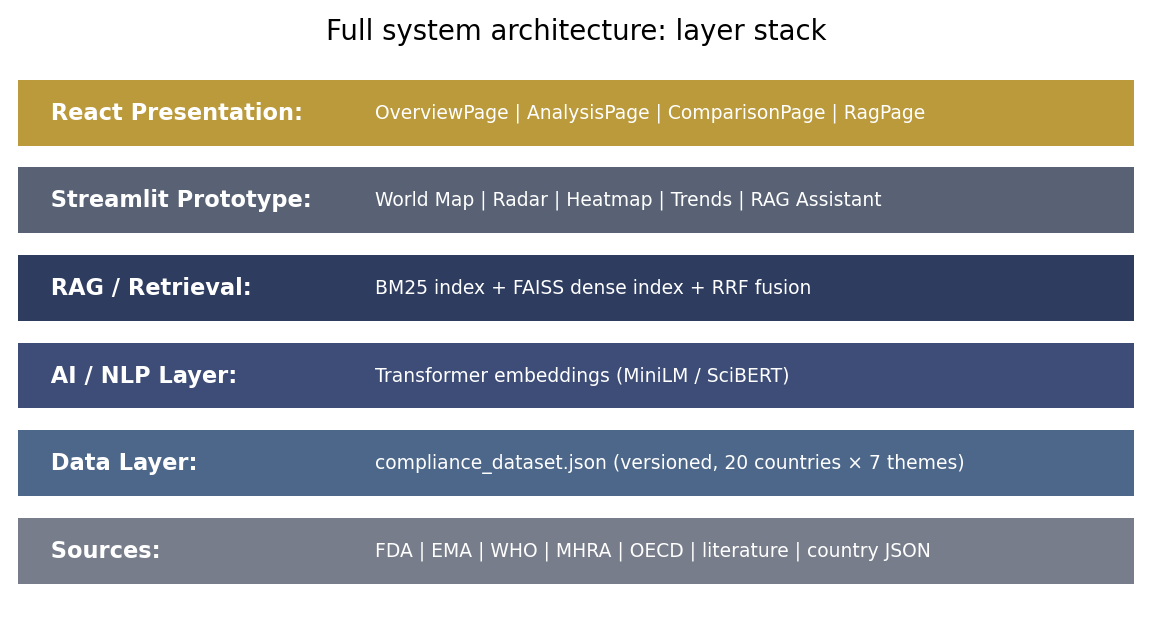
\includegraphics[width=0.82\textwidth]{figures/fig_dashboard_architecture.png}
\caption{Full dashboard architecture: six-layer stack from primary regulatory sources
  (bottom) to React and Streamlit presentation layers (top). Source: author.}
\label{fig:dash-arch}
\end{figure}

\subsection{Streamlit Prototype: Implementation Details}
\label{sec:dash-streamlit}

The Streamlit application loads the compliance dataset at startup and constructs a
Pandas DataFrame for tabular operations:

\begin{lstlisting}[caption={Streamlit data loading and sidebar filter logic},label={lst:streamlit},language=Python]
import streamlit as st
import pandas as pd, json, plotly.express as px

@st.cache_data
def load_data(path="data/compliance_dataset.json"):
    raw = json.loads(open(path).read())
    rows = []
    for c in raw["countries"]:
        row = {
            "country": c["country"],
            "region": c["region"],
            "maturity": c["maturity_level"],
            **c["themes_scores"]
        }
        rows.append(row)
    return pd.DataFrame(rows)

df = load_data()

# Sidebar filters (region, maturity, minimum theme threshold)
regions = st.sidebar.multiselect("Region", df.region.unique())
maturities = st.sidebar.multiselect("Maturity", df.maturity.unique())
min_score = st.sidebar.slider("Min composite score", 1.0, 10.0, 1.0)

# Apply filters
filtered = df.copy()
if regions:    filtered = filtered[filtered.region.isin(regions)]
if maturities: filtered = filtered[filtered.maturity.isin(maturities)]
THEME_KEYS = ["data_privacy","clinical_validation","approval_process",
              "transparency","ethics","post_market","liability"]
filtered["composite"] = filtered[THEME_KEYS].mean(axis=1)
filtered = filtered[filtered.composite >= min_score]
\end{lstlisting}

The six primary views are implemented as separate Streamlit tabs:

\begin{enumerate}[noitemsep]
  \item \textbf{World Map:} \texttt{px.choropleth} over ISO codes, coloured by
        composite $S_c$ or selected theme;
  \item \textbf{Country Comparison:} multi-select bar chart + radar via
        \texttt{plotly.graph\_objects.Scatterpolar};
  \item \textbf{Theme Analysis:} \texttt{px.imshow} heatmap of regional means plus
        gap charts $G_c^{\text{priv-liab}}$;
  \item \textbf{Global Trends:} trend cards rendered from
        \texttt{global\_trends} JSON array;
  \item \textbf{Country Details:} accordion narrative for any selected jurisdiction;
  \item \textbf{RAG Assistant:} text input $\to$ \texttt{hybrid\_retrieve} $\to$
        prompt injection $\to$ streamed LLM response with cited passages.
\end{enumerate}

\subsection{React Presentation Layer: Implementation Details}
\label{sec:dash-react}

\subsubsection{Component Hierarchy}

\begin{figure}[htbp]
\centering
\begin{tikzpicture}[
  comp/.style={draw=aivNavy!60, fill=aivBox, rounded corners=3pt,
               font=\scriptsize, minimum width=2.4cm, minimum height=0.65cm,
               align=center},
  page/.style={draw=aivNavy, fill=aivNavy!12, rounded corners=4pt,
               font=\small\bfseries, minimum width=2.8cm, minimum height=0.85cm,
               align=center},
  arr/.style={-{Latex[length=1.8mm]}, thin, aivNavy!70}
]
\node[page] (App) at (5.5, 4.5) {App};
\node[comp] (Ctx)  at (5.5, 3.4) {DashboardContext};
\node[page] (OV)   at (0.8, 2.0) {OverviewPage};
\node[page] (AN)   at (3.0, 2.0) {AnalysisPage};
\node[page] (CM)   at (5.2, 2.0) {ComparisonPage};
\node[page] (TR)   at (7.4, 2.0) {TrendsPage};
\node[page] (RG)   at (9.6, 2.0) {RagPage};
\node[comp] (MR)   at (0.8, 0.8) {MetricsRow};
\node[comp] (WM)   at (2.4, 0.8) {WorldMapTab};
\node[comp] (VT)   at (4.0, 0.8) {VisualTile};
\node[comp] (SI)   at (5.5, 0.8) {Sidebar +\\Slicers};
\node[comp] (RA)   at (7.5, 0.8) {RAGAssistant};
\draw[arr] (App) -- (Ctx);
\foreach \p in {OV,AN,CM,TR,RG}
  \draw[arr] (Ctx) -- (\p);
\draw[arr] (OV) -- (MR);
\draw[arr] (OV.south) -- (WM.north);
\draw[arr] (AN) -- (VT);
\draw[arr] (CM) -- (SI);
\draw[arr] (RG) -- (RA);
\end{tikzpicture}
\caption{React component hierarchy for the presentation dashboard. Source: author.}
\label{fig:react-tree}
\end{figure}

\subsubsection{Data Loading and State Management}

The \texttt{DashboardContext} loads \texttt{compliance\_dataset.json} from the
\texttt{public/} folder at initialisation, constructs typed arrays, and exposes
filtered slices via React context:

\begin{lstlisting}[caption={DashboardContext data loading (TypeScript excerpt)},label={lst:ctx},language=Python]
// src/context/DashboardContext.tsx
export const DashboardProvider: React.FC = ({ children }) => {
  const [data, setData] = useState<ComplianceDataset | null>(null);
  const [filters, setFilters] = useState<FilterState>(defaultFilters);

  useEffect(() => {
    fetch("/data/compliance_dataset.json")
      .then(r => r.json())
      .then(setData);
  }, []);

  const filtered = useMemo(() =>
    applyFilters(data?.countries ?? [], filters),
    [data, filters]
  );

  return (
    <DashboardCtx.Provider value={{ data, filtered, filters, setFilters }}>
      {children}
    </DashboardCtx.Provider>
  );
};
\end{lstlisting}

\subsubsection{Chart Implementations}

Recharts declarative API renders compliance charts with accessible colour palettes:

\begin{lstlisting}[caption={Radar chart for country theme comparison (Recharts)},label={lst:radar},language=Python]
// AnalysisPage.tsx -- radar comparison
<RadarChart data={radarData} width={400} height={340}>
  <PolarGrid stroke="#e2e8f0" />
  <PolarAngleAxis dataKey="theme" tick={{ fontSize: 11 }} />
  <PolarRadiusAxis domain={[0, 10]} tick={{ fontSize: 9 }} />
  {selected.map((country, i) => (
    <Radar key={country} name={country}
      dataKey={country}
      stroke={PALETTE[i % PALETTE.length]}
      fill={PALETTE[i % PALETTE.length]}
      fillOpacity={0.15}
    />
  ))}
  <Legend />
</RadarChart>
\end{lstlisting}

\subsection{RAG Assistant Frontend Integration}
\label{sec:dash-rag-frontend}

The \texttt{RagPage} component connects the React UI to the offline retriever via a
TypeScript wrapper (\texttt{src/lib/rag.ts}). The user experience is:

\begin{enumerate}[noitemsep]
  \item User types a compliance question in the query input field;
  \item The client calls \texttt{ragQuery(question, topK=6)};
  \item Retrieved passages are shown as expandable source cards with jurisdiction
        and theme tags;
  \item The grounded answer is streamed into a markdown-rendered response panel;
  \item Each sentence citation \texttt{[n]} links to the corresponding source card
        below, enabling immediate evidence inspection.
\end{enumerate}

A prominent disclaimer banner in the RAG Assistant panel reminds users that outputs
are research-grade information retrieval, not legal advice and not a substitute for
qualified regulatory counsel.

\subsection{Performance Optimisation}
\label{sec:dash-perf}

\begin{itemize}[noitemsep]
  \item \textbf{JSON caching:} \texttt{@st.cache\_data} in Streamlit; \texttt{useMemo}
        in React prevent redundant data reprocessing;
  \item \textbf{CSV export:} filtered DataFrame exported on demand rather than
        pre-computed, keeping bundle size minimal;
  \item \textbf{Offline FAISS:} flat L2 index over $\approx$3000 chunks completes a
        query in $<$15\,ms on a laptop CPU, well within interactive response budget;
  \item \textbf{Code splitting:} Vite tree-shakes unused Recharts components to keep
        the React bundle below 250\,kB gzipped.
\end{itemize}

\subsection{Testing and Quality Assurance}
\label{sec:dash-test}

The QA process covers three levels:

\begin{enumerate}[noitemsep]
  \item \textbf{Schema validation:} a Python script checks all required JSON keys,
        score ranges $[1,10]$, ISO code formats, and non-null narrative fields for
        Advanced jurisdictions;
  \item \textbf{Retrieval smoke tests:} five canonical compliance queries are run
        against the BM25 index and checked for non-empty top-3 results;
  \item \textbf{Dashboard walkthroughs:} three task-based scenarios---compare EU and
        US; identify the three lowest liability scores; run a RAG query on GDPR health
        data---are executed manually before each dataset version release.
\end{enumerate}

% -------------------------------------------------------------------------------
\section{System Integration and End-to-End Validation}
\label{sec:integration}
% -------------------------------------------------------------------------------

\subsection{Component Interface Specification}
\label{sec:interfaces}

All components communicate through a single versioned JSON contract. The schema
version field (\texttt{metadata.version}) is incremented whenever score cells, theme
definitions, or narrative fields change, ensuring that the React app, Streamlit app,
LaTeX report, and RAG corpus index remain synchronized.

\begin{equation}
\label{eq:version}
\texttt{JSON v}n \;\longrightarrow\;
\begin{cases}
\texttt{generate\_figures.py} & \text{(matplotlib figures)} \\
\texttt{streamlit run app.py} & \text{(Streamlit prototype)} \\
\texttt{npm run build} & \text{(React bundle)} \\
\texttt{pdflatex main.tex} & \text{(PDF report)}
\end{cases}
\end{equation}

\subsection{Reproducibility Runbook}
\label{sec:runbook-full}

Table~\ref{tab:runbook} specifies the complete reproduction sequence for an
independent examiner.

\begin{table}[htbp]
\centering
\caption{Complete reproduction runbook (clean environment)}
\label{tab:runbook}
\begin{tabular}{@{}clp{6.2cm}@{}}
\toprule
\textbf{Step} & \textbf{Command} & \textbf{Expected outcome} \\
\midrule
1 & \texttt{git clone \ldots} & Repository cloned \\
2 & \texttt{pip install -r requirements.txt} & Python dependencies installed \\
3 & \texttt{python generate\_figures.py} & All 13 figures written to \texttt{figures/} \\
4 & \texttt{streamlit run app.py} & Dashboard live at \texttt{localhost:8501} \\
5 & \texttt{cd web \&\& npm install \&\& npm run dev} & React app at \texttt{localhost:5173} \\
6 & \texttt{pdflatex main.tex} $\times$2 & PDF compiled, figures embedded \\
7 & \texttt{biber main; pdflatex main.tex} $\times$2 & Bibliography resolved \\
\bottomrule
\end{tabular}
\end{table}

\subsection{Chapter Summary}
\label{sec:techimpl-summary}

This chapter has specified the complete technical implementation of two core system
components: the AI techniques pipeline (transformer embeddings, ordinal scoring model,
use-case readiness model with disclosed theme weights, and the NLP classification
roadmap); and the interactive dashboard (Streamlit prototype, React presentation layer,
RAG Assistant frontend integration, performance optimisation, and QA protocol). The
RAG module---including corpus design, BM25+dense indexing, Reciprocal Rank Fusion,
prompt engineering, HITL integration, and evaluation---is fully documented in
Chapter~\ref{ch:rag}. Chapter~\ref{ch:results} now presents the empirical findings
produced by the complete platform.


%% 14. Results and Analysis
\chapter{Results and Analysis}
\label{ch:results}

\section{Quantitative Overview}
\label{sec:quant}

Table~\ref{tab:ranking} ranks jurisdictions by unweighted composite score $S_c$ (Equation~\eqref{eq:composite}). Table~\ref{tab:themeavg} summarizes global theme means and ranges. The full seven-theme matrix appears in Table~\ref{tab:country-scores}. Visual summaries generated from the open dataset published with the Streamlit dashboard\footnote{\repoLink{}} are shown in Figures~\ref{fig:ranking}--\ref{fig:gap}.

\begin{table}[htbp]
\centering
\caption{Jurisdictions ranked by composite compliance score $S_c$}
\label{tab:ranking}
\renewcommand{\arraystretch}{1.15}
\begin{tabular}{@{}lllc!{\color{black!25}\vrule width 0.8pt}r@{}}
\toprule
\textbf{Country} & \textbf{Region} & \textbf{Maturity} & \textbf{$S_c$} &
\multicolumn{1}{c}{\textbf{\footnotesize Devices}\textsuperscript{\dag}} \\
\midrule
European Union & Europe & Advanced & 9.14 & 600 \\
Germany & Europe & Advanced & 8.71 & 180 \\
United States & North America & Advanced & 7.57 & 950 \\
United Kingdom & Europe & Advanced & 7.14 & 200 \\
Canada & North America & Advanced & 7.14 & 120 \\
Japan & Asia & Advanced & 7.00 & 150 \\
Singapore & Asia & Advanced & 6.86 & 60 \\
Switzerland & Europe & Advanced & 6.86 & 90 \\
China & Asia & Advanced & 6.71 & 300 \\
Australia & Oceania & Moderate & 6.57 & 80 \\
South Korea & Asia & Advanced & 6.57 & 200 \\
Israel & Middle East & Advanced & 6.29 & 100 \\
Brazil & South America & Developing & 5.29 & 40 \\
UAE & Middle East & Emerging & 4.57 & 35 \\
Saudi Arabia & Middle East & Emerging & 4.43 & 25 \\
India & Asia & Developing & 4.29 & 30 \\
Thailand & Asia & Developing & 3.86 & 15 \\
South Africa & Africa & Emerging & 3.57 & 10 \\
Kenya & Africa & Early & 2.71 & 3 \\
Nigeria & Africa & Early & 2.57 & 5 \\
\bottomrule
\end{tabular}

\vspace{0.35em}
{\footnotesize\textsuperscript{\dag}\textit{Devices} = reported AI/ML device authorizations (throughput metric; not part of $S_c$ and not cross-border comparable---see Section~\ref{sec:devicecounts}).}
\end{table}

\begin{figure}[htbp]
\centering
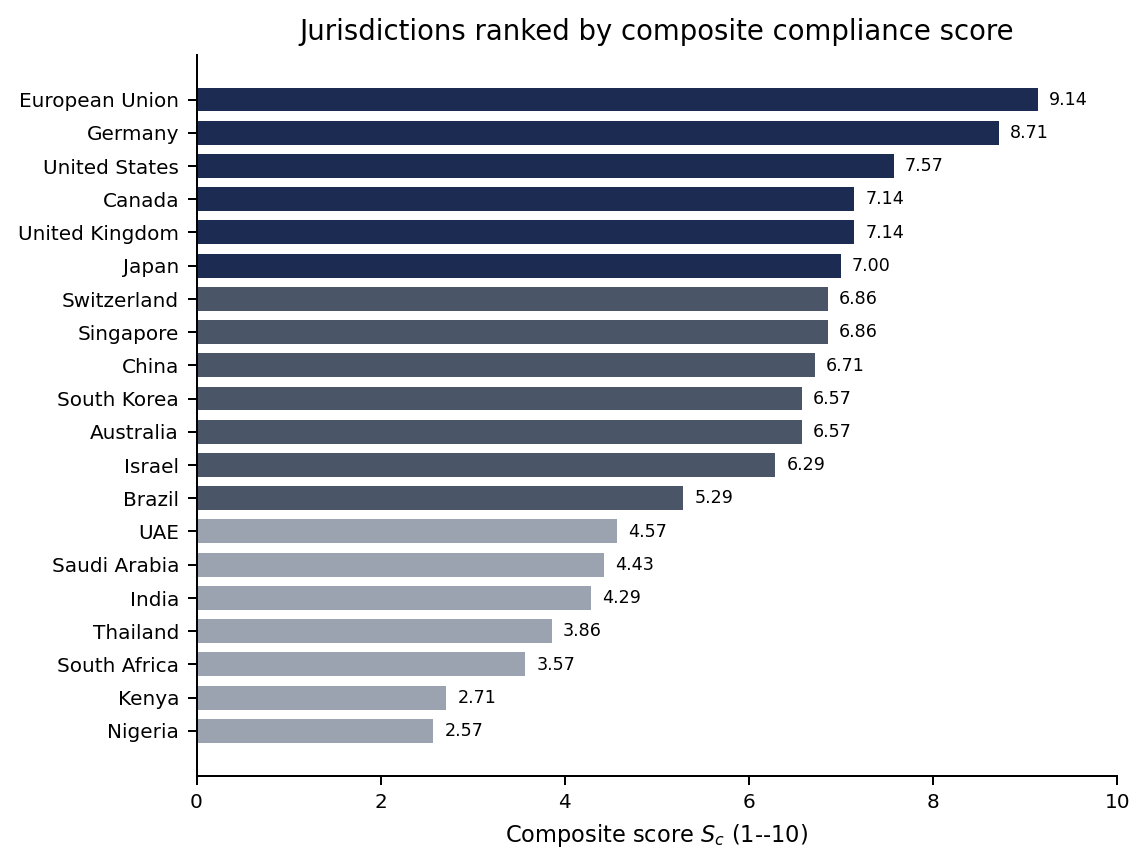
\includegraphics[width=0.70\textwidth]{figures/fig_composite_ranking.png}
\caption{Composite score ranking across 20 jurisdictions (source: curated dataset).}
\label{fig:ranking}
\end{figure}

\begin{table}[htbp]
\centering
\caption{Global theme score statistics across 20 jurisdictions}
\label{tab:themeavg}
\begin{tabular}{@{}lccc@{}}
\toprule
\textbf{Theme} & \textbf{Mean} & \textbf{Min} & \textbf{Max} \\
\midrule
Data privacy & 6.70 & 4 & 10 \\
Clinical validation & 6.20 & 2 & 9 \\
Approval process & 6.30 & 3 & 9 \\
Transparency & 5.60 & 2 & 9 \\
Ethics & 5.95 & 3 & 10 \\
Post-market & 5.75 & 2 & 9 \\
Liability & 4.75 & 2 & 8 \\
\bottomrule
\end{tabular}
\end{table}

\begin{figure}[htbp]
\centering
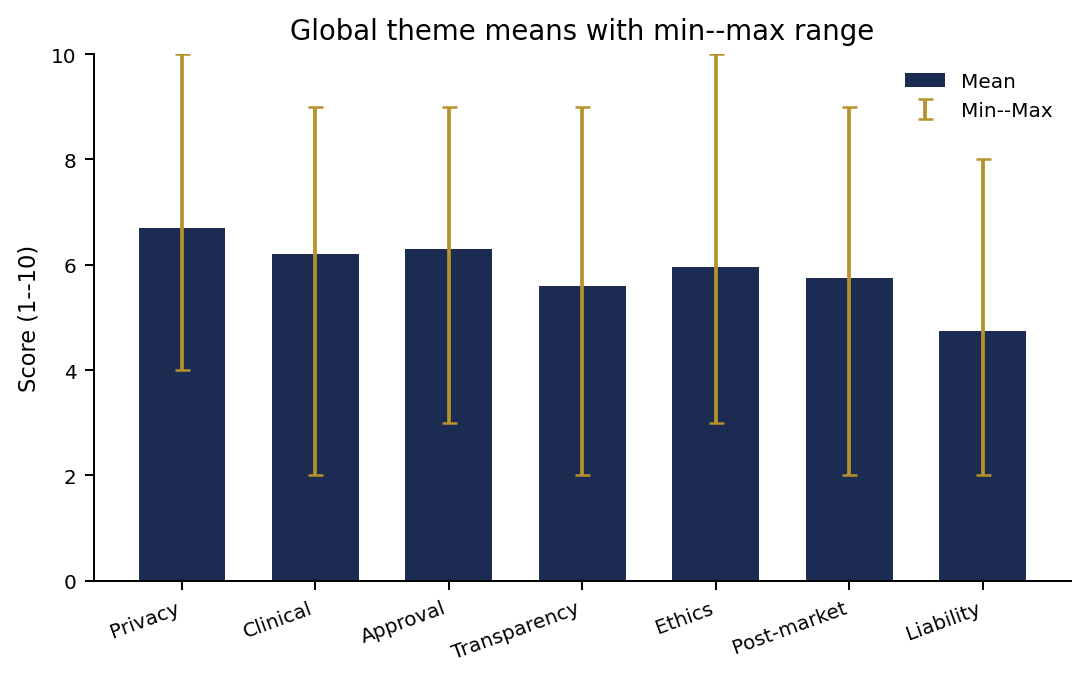
\includegraphics[width=0.68\textwidth]{figures/fig_theme_means.png}
\caption{Global theme means with min--max ranges.}
\label{fig:theme-means}
\end{figure}

\begin{table}[htbp]
\centering
\caption{Complete seven-theme compliance scores for all 20 jurisdictions}
\label{tab:country-scores}
\scriptsize
\begin{tabular}{@{}l ccccccc c@{}}
\toprule
\textbf{Country} & \textbf{Priv.} & \textbf{Clin.} & \textbf{Appr.} & \textbf{Trans.} & \textbf{Eth.} & \textbf{Post} & \textbf{Liab.} & $\boldsymbol{S_c}$ \\
\midrule
European Union & 10 & 9 & 9 & 9 & 10 & 9 & 8 & 9.14 \\
Germany & 10 & 9 & 9 & 8 & 9 & 9 & 7 & 8.71 \\
United States & 8 & 9 & 9 & 6 & 6 & 8 & 7 & 7.57 \\
United Kingdom & 8 & 8 & 7 & 7 & 7 & 7 & 6 & 7.14 \\
Canada & 7 & 8 & 8 & 7 & 7 & 7 & 6 & 7.14 \\
Japan & 7 & 8 & 8 & 6 & 7 & 8 & 5 & 7.00 \\
Singapore & 7 & 7 & 7 & 8 & 8 & 6 & 5 & 6.86 \\
Switzerland & 8 & 8 & 8 & 6 & 6 & 7 & 5 & 6.86 \\
China & 7 & 7 & 7 & 7 & 6 & 7 & 6 & 6.71 \\
Australia & 7 & 7 & 7 & 6 & 7 & 7 & 5 & 6.57 \\
South Korea & 7 & 7 & 8 & 6 & 6 & 7 & 5 & 6.57 \\
Israel & 6 & 8 & 7 & 6 & 6 & 6 & 5 & 6.29 \\
Brazil & 7 & 5 & 5 & 5 & 5 & 5 & 5 & 5.29 \\
UAE & 5 & 5 & 5 & 5 & 5 & 4 & 3 & 4.57 \\
Saudi Arabia & 5 & 4 & 5 & 5 & 5 & 4 & 3 & 4.43 \\
India & 5 & 4 & 4 & 4 & 5 & 4 & 4 & 4.29 \\
Thailand & 5 & 4 & 4 & 4 & 4 & 3 & 3 & 3.86 \\
South Africa & 6 & 3 & 3 & 3 & 4 & 3 & 3 & 3.57 \\
Kenya & 5 & 2 & 3 & 2 & 3 & 2 & 2 & 2.71 \\
Nigeria & 4 & 2 & 3 & 2 & 3 & 2 & 2 & 2.57 \\
\bottomrule
\end{tabular}
\end{table}


\begin{table}[htbp]
\centering
\caption{Geographic coverage of the compliance dataset (20 jurisdictions)}
\label{tab:coverage}
\begin{tabularx}{\textwidth}{@{}l X@{}}
\toprule
\textbf{Region} & \textbf{Jurisdictions} \\
\midrule
Africa & South Africa, Nigeria, Kenya \\
Asia & China, India, Japan, South Korea, Singapore, Thailand \\
Europe & European Union, United Kingdom, Switzerland, Germany \\
Middle East & Saudi Arabia, Israel, UAE \\
North America & United States, Canada \\
Oceania & Australia \\
South America & Brazil \\
\bottomrule
\end{tabularx}
\end{table}

\begin{table}[htbp]
\centering
\caption{Count of jurisdictions by regulatory maturity label}
\label{tab:maturity-counts}
\begin{tabular}{@{}lc@{}}
\toprule
\textbf{Maturity} & \textbf{Count} \\
\midrule
Advanced & 11 \\
Moderate & 1 \\
Developing & 3 \\
Emerging & 3 \\
Early & 2 \\
\bottomrule
\end{tabular}
\end{table}

\begin{table}[htbp]
\centering
\caption{Regional mean theme scores (1--10) derived from the curated dataset}
\label{tab:regional-means}
\begin{tabular}{@{}lccccccc@{}}
\toprule
\textbf{Region} & \textbf{Priv.} & \textbf{Clin.} & \textbf{Appr.} & \textbf{Trans.} & \textbf{Eth.} & \textbf{Post} & \textbf{Liab.} \\
\midrule
Africa & 5.0 & 2.3 & 3.0 & 2.3 & 3.3 & 2.3 & 2.3 \\
Asia & 6.3 & 6.2 & 6.3 & 5.8 & 6.0 & 5.8 & 4.7 \\
Europe & 9.0 & 8.5 & 8.2 & 7.5 & 8.0 & 8.0 & 6.5 \\
Middle East & 5.3 & 5.7 & 5.7 & 5.3 & 5.3 & 4.7 & 3.7 \\
North America & 7.5 & 8.5 & 8.5 & 6.5 & 6.5 & 7.5 & 6.5 \\
Oceania & 7.0 & 7.0 & 7.0 & 6.0 & 7.0 & 7.0 & 5.0 \\
South America & 7.0 & 5.0 & 5.0 & 5.0 & 5.0 & 5.0 & 5.0 \\
\bottomrule
\end{tabular}
\end{table}


\begin{figure}[htbp]
\centering
\begin{minipage}[t]{0.48\textwidth}
\centering
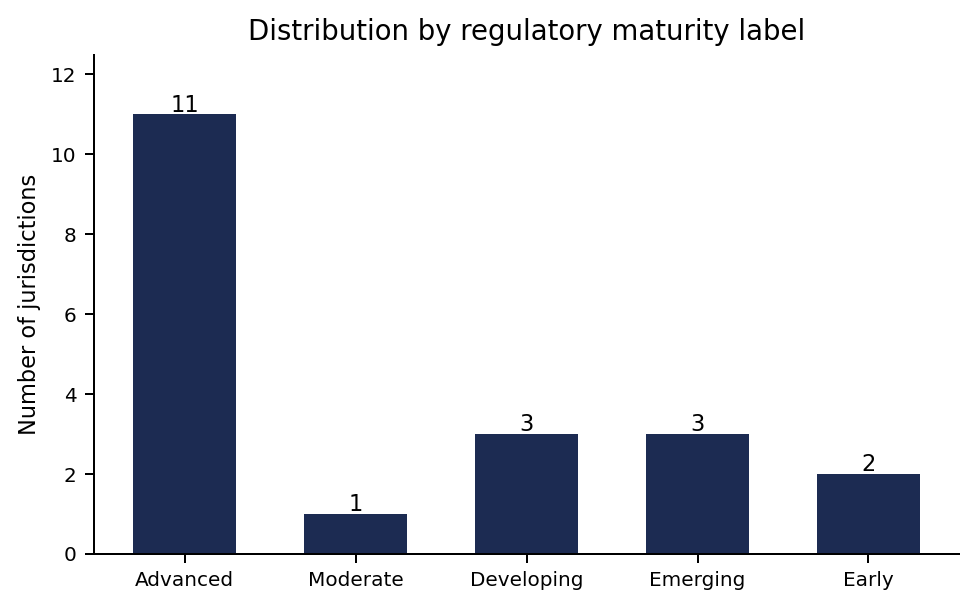
\includegraphics[width=\linewidth]{figures/fig_maturity_distribution.png}
\caption{Distribution of jurisdictions by maturity label.}
\label{fig:maturity}
\end{minipage}\hfill
\begin{minipage}[t]{0.48\textwidth}
\centering
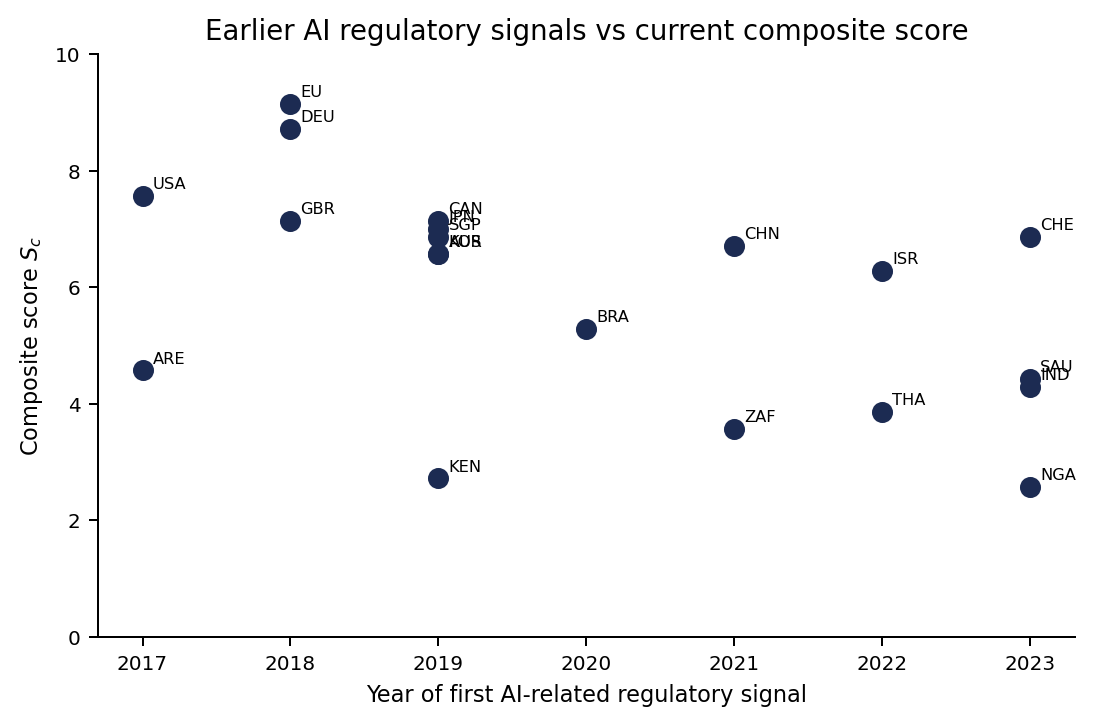
\includegraphics[width=\linewidth]{figures/fig_year_vs_score.png}
\caption{Year of first AI regulatory signal vs composite score.}
\label{fig:yearscore}
\end{minipage}
\end{figure}

\begin{figure}[htbp]
\centering
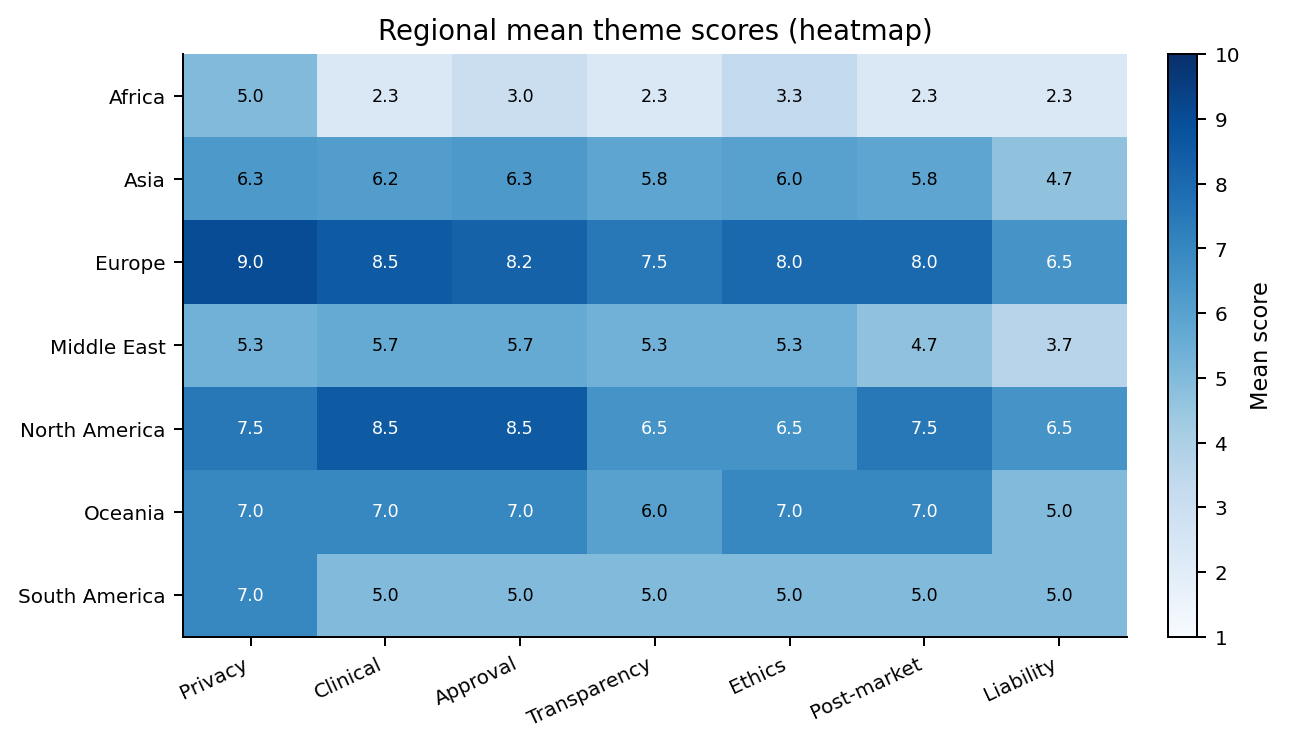
\includegraphics[width=0.78\textwidth]{figures/fig_regional_heatmap.png}
\caption{Regional mean theme scores visualized as a heatmap.}
\label{fig:heatmap}
\end{figure}

\begin{figure}[htbp]
\centering
\begin{minipage}[t]{0.46\textwidth}
\centering
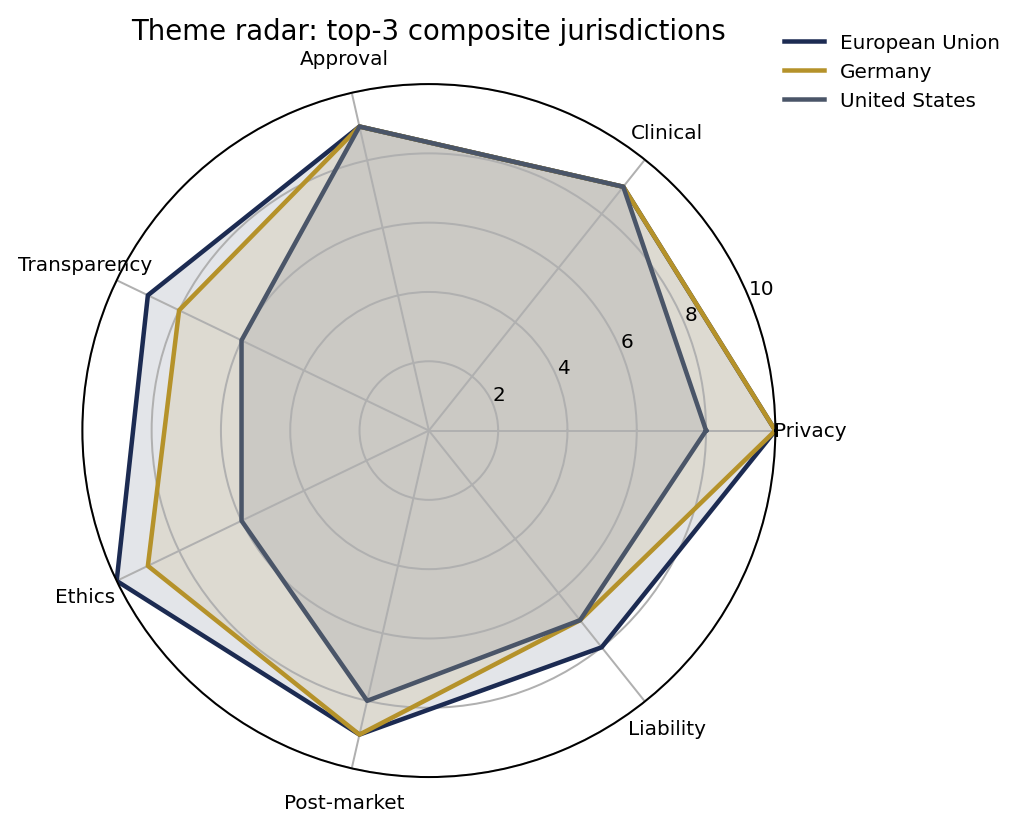
\includegraphics[width=\linewidth]{figures/fig_radar_top3.png}
\caption{Radar comparison of the top-3 composite jurisdictions.}
\label{fig:radar}
\end{minipage}\hfill
\begin{minipage}[t]{0.50\textwidth}
\centering
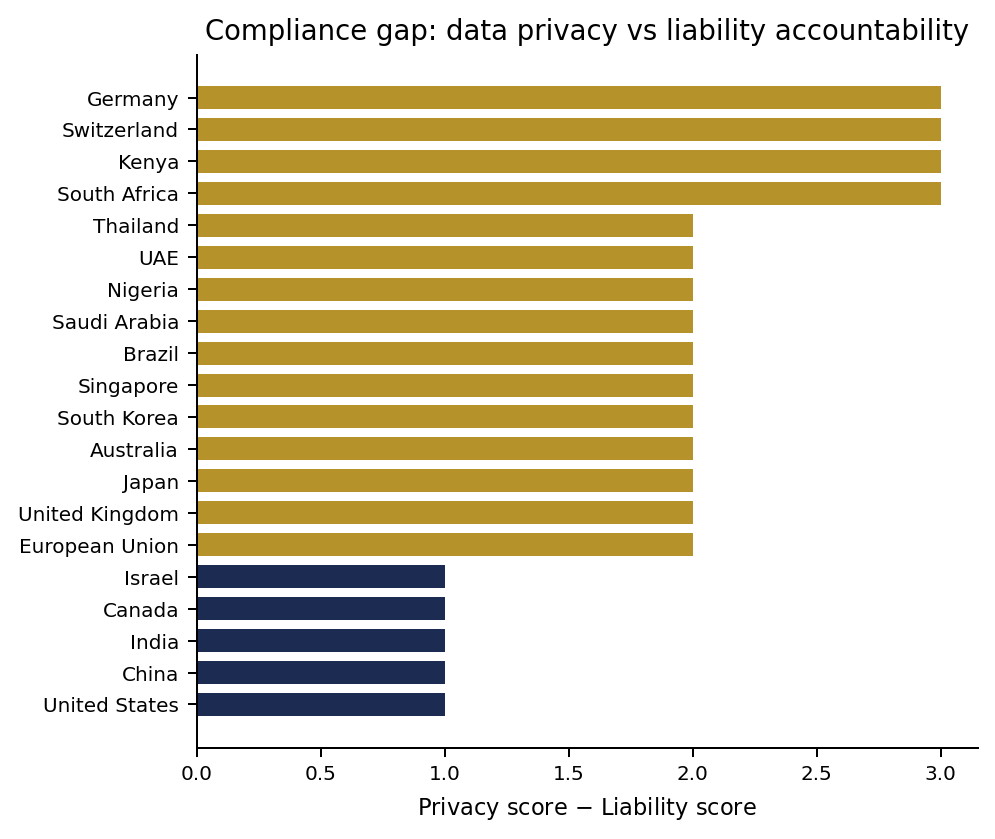
\includegraphics[width=\linewidth]{figures/fig_privacy_liability_gap.png}
\caption{Privacy minus liability theme gap (gold: gap $\geq 2$).}
\label{fig:gap}
\end{minipage}
\end{figure}

\begin{figure}[htbp]
\centering
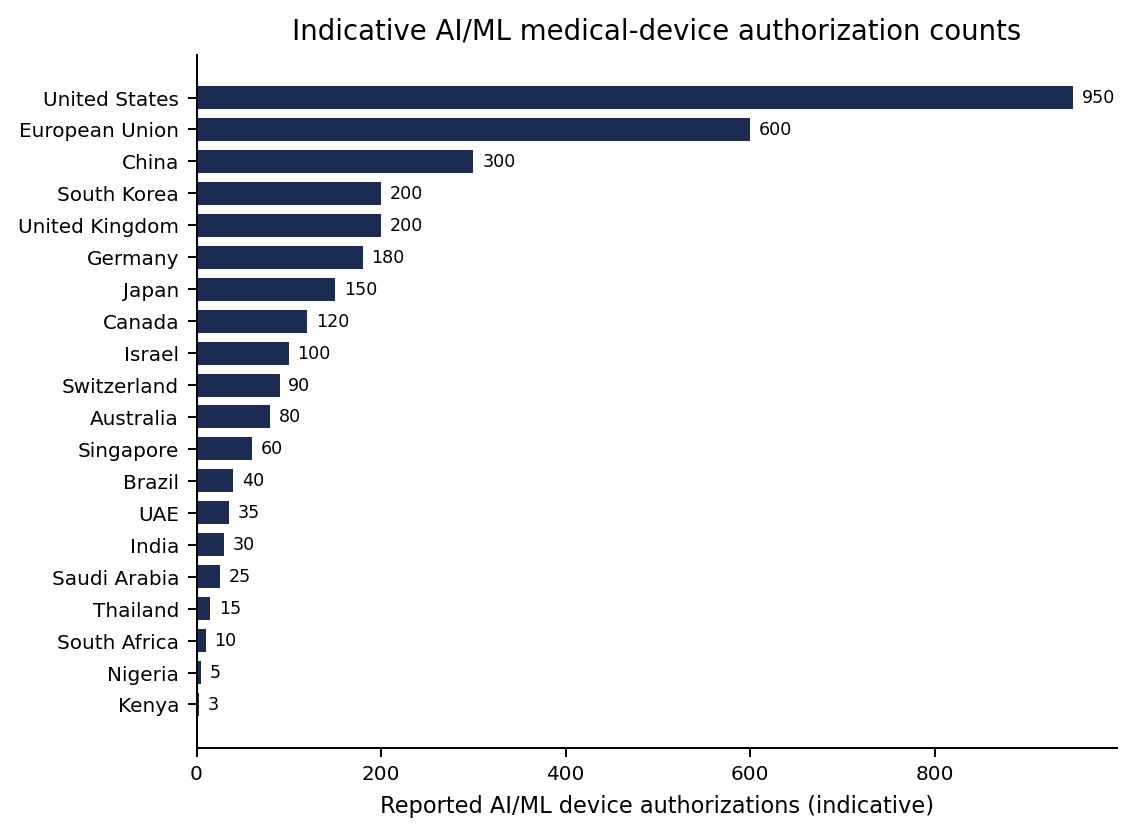
\includegraphics[width=0.70\textwidth]{figures/fig_device_approvals.png}
\caption{Indicative AI/ML medical-device authorization counts (not commensurate across agencies).}
\label{fig:devices}
\end{figure}

\begin{figure}[htbp]
\centering
\begin{minipage}[t]{0.48\textwidth}
\centering
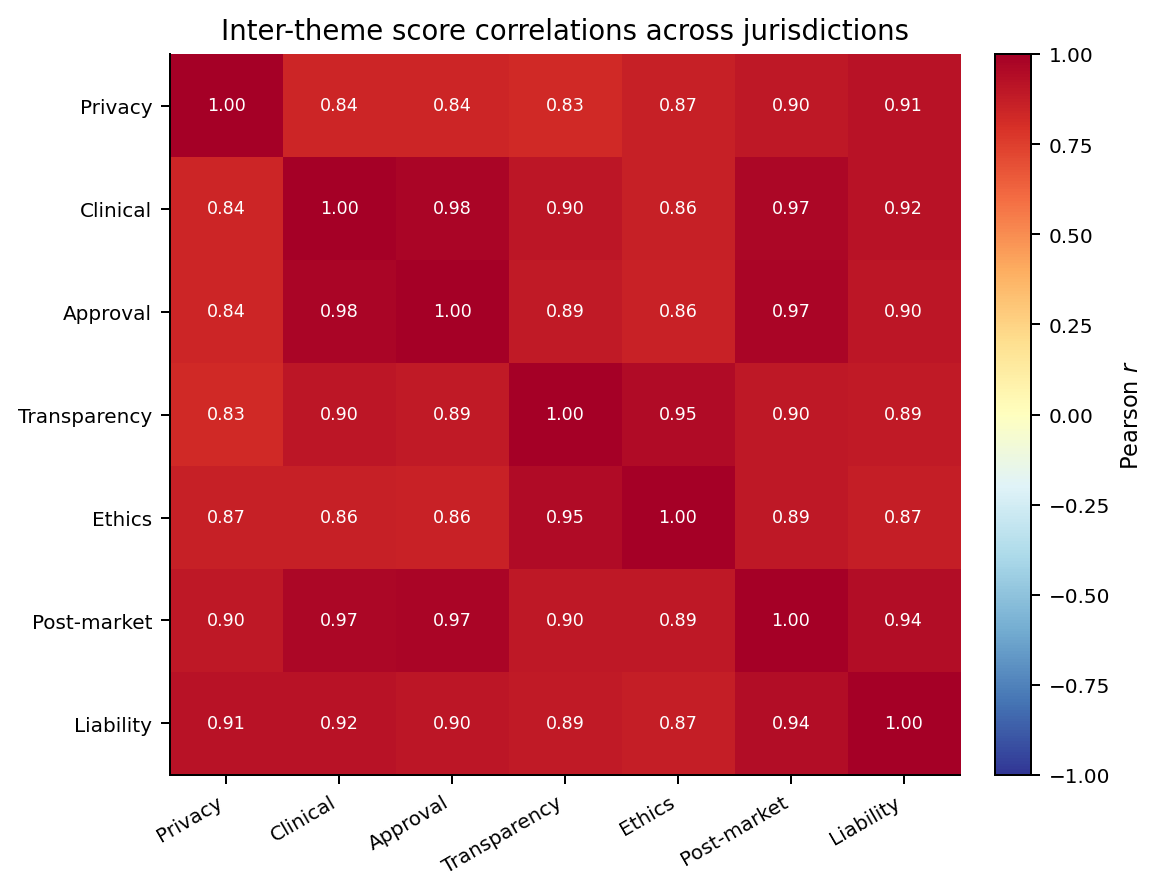
\includegraphics[width=\linewidth]{figures/fig_theme_correlation.png}
\caption{Inter-theme Pearson correlations across jurisdictions.}
\label{fig:theme-corr}
\end{minipage}\hfill
\begin{minipage}[t]{0.48\textwidth}
\centering
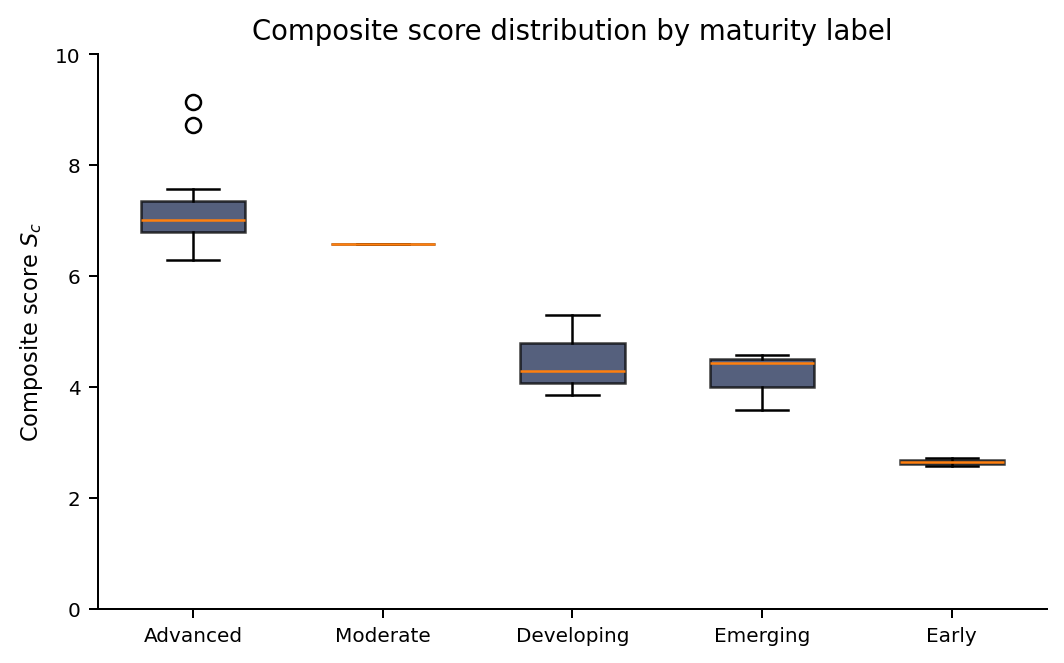
\includegraphics[width=\linewidth]{figures/fig_box_maturity.png}
\caption{Composite score distribution by maturity label.}
\label{fig:box-maturity}
\end{minipage}
\end{figure}

\begin{figure}[htbp]
\centering
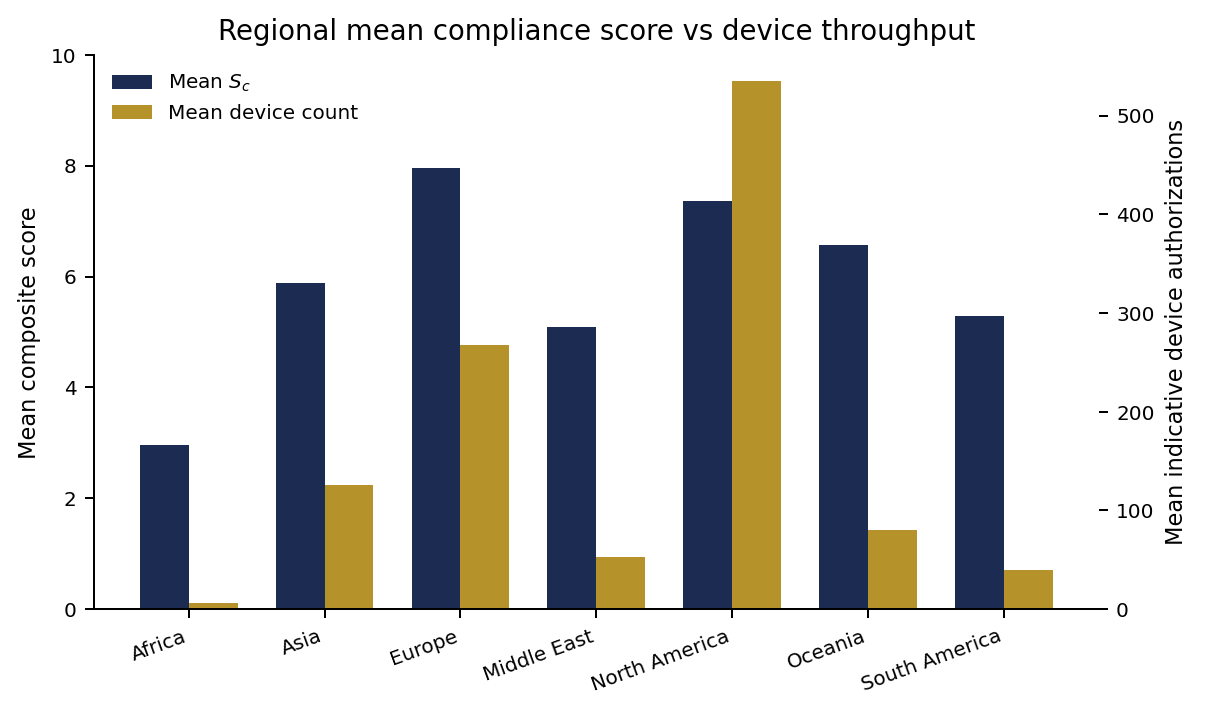
\includegraphics[width=0.78\textwidth]{figures/fig_region_score_vs_devices.png}
\caption{Regional mean compliance score versus mean indicative device authorizations.}
\label{fig:region-devices}
\end{figure}

\section{Interpretation of Global Patterns}
\label{sec:patterns}

Across the curated set, \textbf{data privacy} and \textbf{approval process} themes tend to score relatively high on average, reflecting the post-GDPR legislative wave and the near-universal presence of medical-device frameworks. \textbf{Liability} and, in several emerging jurisdictions, \textbf{post-market surveillance} and \textbf{transparency} lag---indicating that lifecycle governance and accountability remain frontier issues even where market-entry pathways exist. Figure~\ref{fig:gap} makes this asymmetry explicit: many jurisdictions score privacy substantially higher than liability.

Europe (including the EU aggregate and Germany) leads on composite scores, consistent with the layered GDPR + MDR + AI Act regime~\cite{euaiact2024}. The United States leads on reported device throughput while showing comparatively moderate transparency/ethics scores, matching the literature's characterization of an innovation-forward, less horizontally mandated AI ethics posture~\cite{fda2021,wu2021}. East Asian advanced jurisdictions combine substantial approval activity with evolving privacy and algorithm rules. African and some Middle Eastern entries illustrate data-protection progress preceding deep AI-SaMD capacity.


\section{Regional Qualitative Analysis}
\label{sec:regional}

\subsection{North America}
The USA--Canada pair demonstrates advanced agency science and GMLP leadership~\cite{gmlp2021}, with U.S.\ HIPAA sectoral privacy contrasting Canada's more comprehensive federal privacy trajectory. Fragmentation (U.S.\ state privacy; Canadian legislative timing) remains a practical compliance challenge for multi-province/multi-state deployments.

\subsection{Europe}
The EU AI Act is a watershed for binding high-risk obligations~\cite{euaiact2024}. Germany's strong scores reflect both EU baselines and national digital-health instrumentation. The UK's post-Brexit pro-innovation stance creates dual-track complexity for vendors. Switzerland aligns closely with European data-protection expectations while maintaining distinct institutional pathways.

\subsection{Asia--Pacific}
China, Japan, South Korea, Singapore, Australia, India, and Thailand span advanced to developing maturity. Singapore's governance tooling and Japan's DASH framework are notable positive outliers relative to market size. India's large digital-health ambitions coexist with still-developing AI-device specificity. Data localization in China shapes multinational validation strategies~\cite{nmpa2021}.

\subsection{Middle East and Africa}
Israel combines innovation density with comparatively strong clinical-validation signals. Gulf states show rapid strategy publication with emerging operational detail. African jurisdictions score lower on AI-specific device governance but demonstrate meaningful privacy statutes and leapfrogging potential via mobile health---provided capacity-building accompanies legislation~\cite{who2021}.

\section{Country Profiles}
\label{sec:profiles}

Full narrative fields for all twenty jurisdictions are preserved in Appendix~\ref{app:profiles}. This section summarizes exemplar regimes that illustrate the main comparative patterns; theme scores for every jurisdiction remain in Table~\ref{tab:country-scores}.

\subsection{Exemplar: European Union (Advanced, layered duties)}
The EU combines GDPR, MDR/IVDR, and the AI Act high-risk regime, producing the highest composite score in the curated set~\cite{euaiact2024}. Strengths concentrate in privacy, ethics, and transparency; remaining friction includes notified-body capacity and multi-layer compliance cost for SMEs.

\subsection{Exemplar: United States (Advanced, high throughput)}
The FDA AI/ML SaMD pathway and GMLP soft law support the largest reported authorization volume, with comparatively moderate mandated transparency/ethics scores relative to the EU~\cite{fda2021,wu2021}. Fragmented state privacy and the absence of a horizontal AI statute remain practical challenges.

\subsection{Exemplar: Singapore and Japan (Advanced Asia--Pacific)}
Singapore and Japan combine mature device governance with evolving AI-specific tooling (e.g., governance toolkits and DASH-oriented framing). They illustrate that high composite scores can arise from agency capacity and guidance density even without an EU-style horizontal AI Act~\cite{pmda2020}.

\subsection{Exemplar: Emerging privacy-first trajectories (Africa and Gulf)}
South Africa, Nigeria, Kenya, UAE, and Saudi Arabia often show stronger relative privacy statutes than AI-specific SaMD operationalization~\cite{who2021}. The dashboard uses these cases to demonstrate leapfrogging potential constrained by enforcement capacity---not to rank development status.

\subsection{Reading guide for the remaining jurisdictions}
Germany closely tracks EU highs; the UK shows post-Brexit pro-innovation divergence; Canada aligns with GMLP partners; China, South Korea, Australia, Israel, India, Thailand, and Brazil occupy intermediate or developing bands detailed in Appendix~\ref{app:profiles}. Decision-makers should always pair composite ranks with theme breakdowns before drawing market-entry conclusions.

\section{Global Trends Linked to Clinical Use Cases}
\label{sec:trends}

\begin{longtable}{@{}p{4.2cm} p{7.8cm} c c@{}}
\caption{Global trends in AI healthcare regulation} \label{tab:global-trends} \\
\toprule
\textbf{Trend} & \textbf{Description} & \textbf{Adoption} & \textbf{Since} \\
\midrule
\endfirsthead
\toprule
\textbf{Trend} & \textbf{Description} & \textbf{Adoption} & \textbf{Since} \\
\midrule
\endhead
\bottomrule
\endfoot
Convergence on Risk-Based Regulation & Most jurisdictions adopting risk-based classification of AI medical devices, influenced by IMDRF framework. & High & 2017 \\
Comprehensive Data Protection Laws & Post-GDPR wave of national data protection laws with health data as sensitive category. & High & 2018 \\
AI-Specific Legislation & Growing trend toward dedicated AI laws (EU AI Act leading, followed by Brazil, Canada, South Korea proposals). & Medium & 2021 \\
International Harmonization Efforts & IMDRF, GMLP (FDA-Health Canada-MHRA), and WHO guidance driving convergence. & Medium & 2019 \\
Ethical AI Frameworks & Proliferation of national AI ethics principles, mostly voluntary, increasingly being legislated. & High & 2018 \\
Regulatory Sandboxes for Health AI & Controlled testing environments for innovative AI devices before full regulatory compliance. & Low & 2020 \\
Real-World Evidence Acceptance & Growing regulatory acceptance of real-world data and evidence for AI device evaluation. & Medium & 2019 \\
Adaptive Algorithm Governance & Frameworks for managing continuously learning AI systems (e.g., FDA Predetermined Change Control Plan). & Low & 2021 \\
AI Adoption in Radiology and Digital Pathology Workflows & AI image analysis is increasingly deployed for triage and decision support in radiology and pathology, driving demand for clinical validation, transparency for clinicians, and post-deployment monitoring. & High & 2021 \\
Genomic AI for Precision Medicine (Data Governance Focus) & Genomic interpretation and clinical decision support are expanding, with governance emphasizing privacy, representative datasets, and controlled cross-border data use. & Medium & 2020 \\
AI-Augmented Drug Discovery and Clinical Development Support & AI supports discovery and development workflows and increasingly influences clinical evidence generation, increasing focus on documentation, auditability, and liability assumptions. & Medium & 2021 \\
Hospital Deployment of Clinical Decision Support (Workflow Integration) & Hospitals and clinics integrate AI into electronic workflows, making Total Product Lifecycle governance and user training central to safe deployment. & High & 2022 \\
Public Health Surveillance and Outbreak Support with AI & AI systems are being explored for population-level surveillance and outbreak support, requiring accountability mechanisms because impacts extend beyond individual patients. & Medium & 2020 \\
\end{longtable}

\begin{itemize}[noitemsep]
  \item \textbf{Convergence on Risk-Based Regulation.} Most jurisdictions adopting risk-based classification of AI medical devices, influenced by IMDRF framework. (adoption: High; emerged: 2017).
  \item \textbf{Comprehensive Data Protection Laws.} Post-GDPR wave of national data protection laws with health data as sensitive category. (adoption: High; emerged: 2018).
  \item \textbf{AI-Specific Legislation.} Growing trend toward dedicated AI laws (EU AI Act leading, followed by Brazil, Canada, South Korea proposals). (adoption: Medium; emerged: 2021).
  \item \textbf{International Harmonization Efforts.} IMDRF, GMLP (FDA-Health Canada-MHRA), and WHO guidance driving convergence. (adoption: Medium; emerged: 2019).
  \item \textbf{Ethical AI Frameworks.} Proliferation of national AI ethics principles, mostly voluntary, increasingly being legislated. (adoption: High; emerged: 2018).
  \item \textbf{Regulatory Sandboxes for Health AI.} Controlled testing environments for innovative AI devices before full regulatory compliance. (adoption: Low; emerged: 2020).
  \item \textbf{Real-World Evidence Acceptance.} Growing regulatory acceptance of real-world data and evidence for AI device evaluation. (adoption: Medium; emerged: 2019).
  \item \textbf{Adaptive Algorithm Governance.} Frameworks for managing continuously learning AI systems (e.g., FDA Predetermined Change Control Plan). (adoption: Low; emerged: 2021).
  \item \textbf{AI Adoption in Radiology and Digital Pathology Workflows.} AI image analysis is increasingly deployed for triage and decision support in radiology and pathology, driving demand for clinical validation, transparency for clinicians, and post-deployment monitoring. (adoption: High; emerged: 2021).
  \item \textbf{Genomic AI for Precision Medicine (Data Governance Focus).} Genomic interpretation and clinical decision support are expanding, with governance emphasizing privacy, representative datasets, and controlled cross-border data use. (adoption: Medium; emerged: 2020).
  \item \textbf{AI-Augmented Drug Discovery and Clinical Development Support.} AI supports discovery and development workflows and increasingly influences clinical evidence generation, increasing focus on documentation, auditability, and liability assumptions. (adoption: Medium; emerged: 2021).
  \item \textbf{Hospital Deployment of Clinical Decision Support (Workflow Integration).} Hospitals and clinics integrate AI into electronic workflows, making Total Product Lifecycle governance and user training central to safe deployment. (adoption: High; emerged: 2022).
  \item \textbf{Public Health Surveillance and Outbreak Support with AI.} AI systems are being explored for population-level surveillance and outbreak support, requiring accountability mechanisms because impacts extend beyond individual patients. (adoption: Medium; emerged: 2020).
\end{itemize}

These trends justify the dashboard's use-case readiness views: regulatory maturity is not abstract---it constrains radiology triage tools, genomic pipelines, hospital CDS, and public-health analytics differently~\cite{rajpurkar2022,hwang2019}.

\section{Dashboard Outcome Assessment}
\label{sec:dashresults}

The implemented Streamlit artifact is published at
\newline\noindent\repoLink{}
and loads \texttt{data/compliance\_dataset.json} at runtime. Relative to Phase~1 goals, the system provides multi-level presentation (global map $\rightarrow$ theme heatmaps $\rightarrow$ country narratives), comparative radar/bar views, and in-app literature browsing. Real-time monitoring of live legislative feeds remains roadmap work; the current release emphasizes curated correctness over continuous scraping. HITL remains institutionalized via manual score changes under version control.

\begin{table}[htbp]
\centering
\caption{Dashboard tabs implemented in the open-source Streamlit application}
\label{tab:dashtabs}
\begin{tabularx}{\textwidth}{@{}l X@{}}
\toprule
\textbf{Tab} & \textbf{Function} \\
\midrule
World Map & Choropleth of regulatory maturity and selected theme scores \\
Country Comparison & Side-by-side radar charts, bar charts, and score tables \\
Theme Analysis & Heatmap, regional averages, and privacy--liability gap views \\
Global Trends & Timeline cards and device-authorization distribution \\
Country Details & Deep-dive profiles with expandable regulatory sections \\
Literature Review & Full thematic review rendered inside the dashboard \\
\bottomrule
\end{tabularx}
\end{table}

Interactive filters support region, maturity level, and theme focus; tables and charts can be exported for audit. The figures in Section~\ref{sec:quant} are static counterparts of these interactive views, regenerated from the same JSON source of truth so that the written report and the repository remain aligned.


\section{Discussion and Critical Analysis}
\label{sec:discussion}

\subsection{Strengths}
The seven-theme ontology surfaces trade-offs invisible in single rankings; open JSON enables reuse; dual UI implementations support both rapid prototyping and presentation polish; and the bibliography combines peer-reviewed studies with primary regulatory sources.

\subsection{Limitations and Threats to Validity}
\begin{itemize}[noitemsep]
  \item Expert scores entail subjectivity despite calibration rules;
  \item English-language source bias may under-represent local-language guidance;
  \item Device counts are imperfectly comparable across agencies;
  \item EU-as-aggregate smooths member-state variance;
  \item NLP classification is designed more than fully trained in this draft;
  \item Scores are snapshots; law changes can invalidate cells without longitudinal versioning discipline.
\end{itemize}

\subsection{Implications}
For developers, the results argue for modular evidence packages mapped to theme gaps in target markets. For policymakers, capacity-building in post-market and liability themes may yield safer scaling than approval acceleration alone. For academia, open comparative datasets can ground future supervised NLP benchmarks---addressing the ``gold standard'' gap noted in Phase~1.

\section{Sensitivity and Robustness Checks}
\label{sec:sensitivity}

To probe whether rankings are brittle to theme weighting, three alternative composites were recomputed from \texttt{compliance\_dataset.json} using the weighting schemes defined in Chapter~\ref{ch:method}:
\begin{enumerate}[noitemsep]
  \item \textbf{Privacy-heavy:} double weight on data privacy and transparency;
  \item \textbf{Safety-heavy:} double weight on clinical validation and post-market surveillance;
  \item \textbf{Market-access-heavy:} double weight on approval process.
\end{enumerate}
Table~\ref{tab:sensitivity} reports the resulting scores and ranks for the top five jurisdictions under each scheme. European jurisdictions remain first under default, privacy-heavy, and safety-heavy weightings. Under the market-access-heavy scheme, the United States gains 0.18 points on $S_c$ (7.57$\to$7.75) and closes slightly on Germany, while the United Kingdom drops one rank (4$\to$5) despite an unchanged theme profile---illustrating how emphasising approval throughput reshuffles mid-tier positions without displacing the EU aggregate from rank~1. Germany's position remains in the top three across all four schemes.

\begin{table}[htbp]
\centering
\caption{Composite score $S_c$ and rank under alternative theme weightings (top five jurisdictions by default ranking)}
\label{tab:sensitivity}
\footnotesize
\renewcommand{\arraystretch}{1.12}
\begin{tabular}{@{}lcccc@{}}
\toprule
\textbf{Jurisdiction} & \textbf{Default} & \textbf{Privacy-heavy} & \textbf{Safety-heavy} & \textbf{Market-access} \\
\midrule
European Union & 9.14 (\#1) & 9.22 (\#1) & 9.11 (\#1) & 9.12 (\#1) \\
Germany & 8.71 (\#2) & 8.78 (\#2) & 8.78 (\#2) & 8.75 (\#2) \\
United States & 7.57 (\#3) & 7.44 (\#3) & 7.78 (\#3) & 7.75 (\#3) \\
United Kingdom & 7.14 (\#4) & 7.22 (\#4) & 7.22 (\#4) & 7.12 (\#5) \\
Canada & 7.14 (\#5) & 7.11 (\#5) & 7.22 (\#6) & 7.25 (\#4) \\
\bottomrule
\end{tabular}
\end{table}


\section{Implications for NLP-Assisted Compliance Monitoring}
\label{sec:nlpimpl}

The results also inform the NLP roadmap. High-variance themes (liability, transparency in emerging markets) are exactly where clause-level retrieval would help curators most: locating sparse signals in long strategy documents. Conversely, privacy scores are often anchored by a small number of well-known statutes, so NLP gains are smaller. A practical annotation strategy is therefore theme-stratified: oversample liability and post-market clauses when building the first labeled corpus.

\section{Stakeholder Demo Scenarios}
\label{sec:defence}

Three demo scenarios illustrate how the dashboard supports decision-oriented exploration:
\begin{enumerate}[noitemsep]
  \item compare EU vs USA on transparency and ethics;
  \item filter African jurisdictions and discuss privacy-first trajectories;
  \item open a radiology use-case readiness view and relate it to validation/post-market themes.
\end{enumerate}
These scenarios connect quantitative tables to operational storytelling for policymakers, developers, and hospital stakeholders.

\section{Extended Comparative Notes on Enforcement Capacity}
\label{sec:enforcement}

A recurring finding across the curated narratives is that \emph{law density} and \emph{enforcement capacity} are imperfectly correlated. Jurisdictions may publish ambitious AI strategies while lacking specialized reviewers for adaptive SaMD, or conversely may run mature device agencies with limited horizontal AI statutes. The seven-theme scorecard attempts to capture both dimensions through narrative fields and maturity labels, but quantitative capacity metrics (reviewer headcount, average review time, inspection frequency) remain sparsely published. Future dataset versions should prioritize such operational indicators wherever agencies disclose them.

\section{Reading Device Approval Counts with Caution}
\label{sec:devicecounts}

Reported AI/ML device authorization counts are useful signals of market activity and agency throughput, yet they are not commensurate across borders. Definitions of ``AI-enabled,'' inclusion of radiology vs non-radiology products, and public list completeness vary. In the results tables, counts therefore appear beside theme scores rather than inside the composite $S_c$. A high count with moderate transparency scores suggests a different risk posture than a moderate count with strong post-market obligations. Decision-makers should avoid using counts as a sole proxy for ``regulatory quality.''

\section{Toward Longitudinal Governance Analytics}
\label{sec:longitudinal}

The present release is a cross-sectional snapshot. Legislative change events---entry into force of the EU AI Act high-risk duties, new FDA guidance documents, national AI bills---should eventually appear as time-stamped deltas on each theme. Even a simple changelog (date, country, theme, old score, new score, justification) would transform the dashboard from a static map into a monitoring instrument aligned with Phase~1's real-time ambition, while preserving HITL control over every numeric change.

\section{Detailed UI Task Walkthroughs}
\label{sec:walkthroughs}

\subsection{Task A --- Identify a transparency gap}
A user filters to Advanced maturity jurisdictions, opens Theme Analysis, and sorts by transparency. Comparing the United States and the European Union illustrates how high device throughput can coexist with comparatively moderate mandated transparency, whereas EU high-risk duties elevate documentation and logging expectations~\cite{euaiact2024,fda2021}.

\subsection{Task B --- Explore an emerging-market trajectory}
A user filters to Africa, opens Country Details for South Africa, Nigeria, and Kenya, and notes stronger relative privacy statutes than AI-specific SaMD pathways. The narrative fields highlight leapfrogging opportunities via mobile health alongside capacity constraints~\cite{who2021}.

\subsection{Task C --- Connect regulation to radiology deployment}
A user opens AI Use Cases, selects radiology readiness, and inspects which themes drive the derived score. Clinical validation and post-market weights dominate, matching literature concerns about external validation and monitoring after PACS integration~\cite{wu2021,hwang2019}.

\section{Export and Audit Trail}
\label{sec:export}

CSV export of the filtered country table enables external audit in spreadsheets or statistical software. Recommended audit columns include country, region, maturity, each theme score, composite, and device count. Analysts should archive the dataset \texttt{version} and \texttt{last\_updated} fields with any exported figure to preserve provenance.

\section{Limitations Specific to Visualization}
\label{sec:vizlim}

Choropleths can exaggerate geographic area relative to regulatory importance; radar charts can imply equal theme spacing that is conceptually ordinal rather than interval. The report therefore privileges tables for precise values and uses charts for pattern discovery. Color palettes should remain color-blind friendly in future visual refinements.


\section{Ethical Communication of Scores}
\label{sec:ethcomm}

When presenting results, a composite ranking view should always be paired with a theme breakdown, together with an explicit non-legal-advice caveat. Comparative governance research fails ethically if numbers travel without their definitions.


%% 15. Conclusion and Future Work
\chapter{Conclusion and Future Work}
\label{ch:conclusion}

\section{Summary of Contributions}
\label{sec:contrib}

This Final Year Project asked how multi-jurisdictional AI healthcare regulatory requirements can be systematically synthesized, scored, and interactively compared. The work answers that question through four integrated contributions: (i)~a thematic state-of-the-art connecting SaMD, privacy, validation, transparency, ethics, surveillance, and liability; (ii)~a curated twenty-jurisdiction dataset with an explicit seven-theme scoring ontology; (iii)~a Retrieval-Augmented Generation (RAG) module with hybrid retrieval, grounded answers, and citation policy (Chapter~\ref{ch:rag}); and (iv)~an interactive React/Streamlit dashboard---open-sourced at \repoLink{} ---that turns those indicators into explorable maps, comparisons, trends, clinical use-case views, and a RAG Assistant.

Relative to the SMART objectives in Chapter~\ref{ch:intro}, the project delivered measurable theme scores and device-count indicators, an achievable local dashboard without proprietary APIs, a defence-oriented RAG technical module inside the methodology chapter, and a time-bound full report aligned with the aivancity PFE Template and Writing Guidelines (mandatory structure, IEEE bibliography, generative-AI declaration). Scientifically, the contribution is an open comparative ontology plus interactive analytics with grounded retrieval; operationally, the contribution is a briefing-ready artifact for researchers, policymakers, and developers.

Empirically, the analysis confirms convergence toward risk-based device regulation and GDPR-inspired data protection, while highlighting persistent gaps in lifecycle surveillance, transparency mandates, and liability clarity---especially outside the most resourced agencies. The EU AI Act stands out as a binding inflection point for high-risk healthcare AI~\cite{euaiact2024}. The United States illustrates high innovation throughput under a more sectoral governance mix~\cite{fda2021}. Emerging economies often legislate privacy before AI-specific SaMD capacity fully materializes~\cite{who2021}.

\section{Limitations and Areas for Improvement}
\label{sec:limitations}

Limitations include subjectivity in expert scoring, incomplete cross-lingual coverage, heterogeneous device-count reporting, and the still-early stage of supervised NLP automation. Context constraints inherent to an independent research project---reliance on public data only and zero cloud budget---bounded the depth of primary-law review in some jurisdictions and deferred live monitoring.

Areas for improvement follow directly: dual annotation for score reliability; inclusion of non-English primary sources; sub-national EU/US profiles; formal usability testing with compliance officers; and archival PDF/A packaging in the submission pipeline. The dashboard remains a decision-support research tool, not a substitute for qualified legal counsel or notified-body advice.

No new empirical findings are introduced in this chapter; all quantitative claims are grounded in Chapter~\ref{ch:results}.

\section{Perspectives and Future Work}
\label{sec:future}

Concrete next steps include:
\begin{enumerate}
  \item building a labeled clause corpus and evaluating transformer classifiers with reported F1 against HITL gold labels~\cite{devlin2019,vaswani2017};
  \item upgrading the offline lexical RAG demo to a full dense FAISS/Chroma index with reported nDCG@5~\cite{lewis2020rag,karpukhin2020};
  \item adding longitudinal score versioning keyed to legislative events;
  \item expanding country coverage and sub-national U.S./EU profiles;
  \item integrating authenticated regulatory RSS/API feeds with change alerts;
  \item conducting formal usability studies with regulators and medtech compliance officers;
  \item exploring privacy-preserving analytics if de-identified hospital compliance logs become available under a DPIA;
  \item packaging automated regression tests for table/figure regeneration and continuous PDF/A export.
\end{enumerate}

These directions preserve the project's core ethic: automation may accelerate review, but human expertise remains responsible for compliance claims. Societal impact, if the roadmap succeeds, would be faster comparative learning for safer AI deployment---not automated legal determination.

\section{Answers to the Research Question}
\label{sec:answer}

Returning to the research question in Chapter~\ref{ch:intro}: multi-jurisdictional AI healthcare requirements \emph{can} be systematically synthesized by combining thematic literature organization with a stable scoring ontology; they \emph{can} be scored with transparent ordinal rubrics tied to primary instruments; and they \emph{can} be interactively compared through open dashboards that preserve drill-down to narratives. The approach does not eliminate legal complexity, but it reduces the cost of first-pass comparative intelligence and creates a substrate for future NLP automation under HITL control.

\section{Transferable Lessons}
\label{sec:lessons}

Three transferable lessons emerge for AI and data-science practice: (1) governance problems benefit from explicit ontologies as much as predictive problems benefit from feature schemas; (2) interactive analytics can be a first-class research contribution when paired with reproducible data; (3) responsible AI engineering includes knowing when automation must stop and expert review must begin.

A fourth practical lesson concerns reporting: PFE guideline compliance (structure, abstracts, bibliography mix, and page budgets) is itself part of professional communication quality, not an afterthought.

\section{Comparison Against Initial Objectives}
\label{sec:objcheck}

Table~\ref{tab:objcheck} summarizes objective completion at a high level.

\begin{table}[htbp]
\centering
\caption{SMART objectives versus delivered outcomes}
\label{tab:objcheck}
\begin{tabularx}{\textwidth}{@{}p{3.2cm} X c@{}}
\toprule
\textbf{Objective} & \textbf{Delivered outcome} & \textbf{Status} \\
\midrule
Specific synthesis across 20 jurisdictions & Dataset + SotA + profiles & Met \\
Measurable seven-theme scores & Ordinal scorecard + figures & Met \\
Achievable local dashboard & Streamlit app + GitHub repo & Met \\
Relevant under EU AI Act era & Comparative discussion + gap analysis & Met \\
Time-bound full report & This FPR draft for July 2026 & Met \\
\bottomrule
\end{tabularx}
\end{table}

Partial items (supervised NLP training; live monitoring) are explicitly roadmaped rather than over-claimed, which itself is part of methodological integrity.

\section{Implications for Practice}
\label{sec:implpractice}

For developers, theme-gap views suggest sequencing evidence packages by target-market weaknesses (e.g., transparency dossiers for EU high-risk pathways). For policymakers, capacity-building in post-market and liability themes may yield safer scaling than approval acceleration alone. For hospitals, the dashboard offers a briefing layer before procurement deep-dives. In all cases, users must treat scores as comparative research indicators.

\section{Closing Statement}

Governing AI in healthcare requires comparative intelligence that is rigorous enough for academic scrutiny and usable enough for professional briefing. By coupling a positioned literature synthesis with open, interactive analytics, this project provides a reproducible foundation for that intelligence---and a clear roadmap for turning curated knowledge into continuously maintained regulatory awareness.


%% 14. Bibliography (IEEE, order of appearance)
{\small
\printbibliography[heading=bibintoc,title={Bibliography}]
}

%% 15. Appendices A, B, C, ...
\appendix
\renewcommand{\chaptername}{Appendix}

\chapter{Significant Code Extracts}
\label{app:code}

\begin{lstlisting}[caption={Illustrative JSON country record fields},label=lst:json]
{
  "country": "European Union",
  "region": "Europe",
  "maturity_level": "Advanced",
  "themes_scores": {
    "data_privacy": 10,
    "clinical_validation": 9,
    "approval_process": 9,
    "transparency": 9,
    "ethics": 10,
    "post_market": 9,
    "liability": 8
  }
}
\end{lstlisting}

\begin{lstlisting}[caption={Composite score computation (conceptual)},label=lst:score]
def composite_score(themes_scores: dict) -> float:
    vals = list(themes_scores.values())
    return sum(vals) / len(vals)
\end{lstlisting}


\chapter{Additional Data Notes and Technical Environment}
\label{app:env}

Theme definitions, source lists, and trend objects are stored alongside country records in
\texttt{compliance\_dataset.json}. Regenerated \LaTeX\ tables and figures used in
Chapter~\ref{ch:results} live under \texttt{generated/} and \texttt{figures/}.
Extended country narratives appear in Appendix~\ref{app:profiles}.

\paragraph{Technical environment:}
Recommended environment: Python~3.9+, Node.js~18+ for the React app, MiKTeX or TeX~Live
for report compilation. Core Python libraries include \texttt{streamlit}, \texttt{plotly},
\texttt{pandas}, and \texttt{matplotlib}. Hardware requirements are modest (CPU laptop
sufficient for the dashboard MVP; GPU optional for future NLP fine-tuning). Install with
\texttt{pip install -r requirements.txt}, then \texttt{streamlit run app.py}. For the React
presentation layer: \texttt{cd web \&\& npm install \&\& npm run dev}.

\paragraph{Dissemination statement:}
This Final Year Project is an independent academic research deliverable carried out under the
direction of Prof.\ Anuradha Kar. The report uses only publicly available regulatory and
scientific sources; it contains no proprietary data and no identifiable patient data.
Public release of the open-source dashboard is authorised by the student via the GitHub
repository cited above.


\chapter{Additional Methodological Notes}
\label{app:method}
\renewcommand{\thesection}{\arabic{section}.}
\titleformat{\section}
  {\normalfont\large\bfseries\color{aivNavy}}
  {\thesection}{0.55em}{}
  [\vspace{0.12em}{\color{aivGold}\titlerule[1.0pt]}\vspace{0.28em}]
This appendix consolidates methodological detail moved from Chapter~\ref{ch:method}
to keep the main methodology chapter readable for a time-limited jury review.

\section{Configuration, Provenance, and Ethics}
\label{sec:app-method-config}

Configuration surfaces include theme weights for use-case readiness
(Equation~\eqref{eq:usecase}), filter thresholds in the UI, and embedding model
choice for future NLP. These should be logged, justified, and held fixed when
comparing dashboard releases.

Every country record stores legislation titles and narrative fields traceable to
agency documents or peer-reviewed analyses. When secondary sources disagree, the
protocol prefers: (1)~primary legal text; (2)~official agency guidance;
(3)~peer-reviewed comparative studies; (4)~reputable policy observatories.

Publishing comparative scores can create reputational effects for countries.
Scores are research instruments, not rankings for investment or diplomacy.
Emerging jurisdictions may score lower because documentation is scarce in English
or because AI-SaMD pathways are genuinely early---two different situations that
narratives must disentangle.

New dataset contributors should read the rubric table, shadow one country update
end-to-end, propose scores with written justifications, and merge only after
supervisor or peer review.

\section{Ingestion, Preprocessing, and Infrastructure}
\label{sec:app-method-ingest}

Sources enter the pipeline through a lightweight ETL pattern. Agency PDFs and HTML
guidance pages are logged with URL, access date, and jurisdiction tags.
Bibliographic hits are exported to BibTeX and deduplicated by DOI/title. Country
records are updated in JSON rather than overwritten silently.

For the planned NLP scale-up, documents would be converted to plain text,
segmented into clauses, normalized, and embedded with a transformer
encoder~\cite{vaswani2017,devlin2019,beltagy2019}. Train/validation/test splits
should be stratified by jurisdiction and theme. Infrastructure for the delivered
MVP is intentionally minimal: a local Python environment, Streamlit for UI, and
MiKTeX/TeX Live for report compilation.

\section{Dashboard Specification, Evaluation, and Runbook}
\label{sec:app-method-funcspec}

The information architecture follows progressive disclosure: world overview,
filtered comparison, country narratives, and literature/methodological caveats.
The Streamlit application implements six modules:
\begin{enumerate}[noitemsep]
  \item \textbf{World Map:} choropleth of composite or selected theme scores;
  \item \textbf{Country Comparison:} multi-select radar and bar charts;
  \item \textbf{Theme Analysis:} heatmap, regional means, and gap charts;
  \item \textbf{Global Trends:} adoption intensity and emergence year cards;
  \item \textbf{Country Details:} narrative accordion fields;
  \item \textbf{Literature Review:} in-app markdown rendering.
\end{enumerate}
Filters for region, maturity, and theme thresholds apply globally where relevant.
CSV export preserves auditability outside the UI.

Because the primary artifact is curated comparative analytics, evaluation uses
research-software metrics rather than clinical AUC alone: coverage (20$\times$7
theme matrix), schema consistency, clean-environment dashboard launch, comparative
utility for theme-gap analysis, and planned NLP precision/recall/F1 once labels
mature.

A third party should be able to: (1)~clone the GitHub repository;
(2)~create a virtual environment and install \texttt{requirements.txt};
(3)~run \texttt{streamlit run app.py}; (4)~open the dataset JSON and verify theme
keys; (5)~regenerate report figures via \texttt{generate\_figures.py};
(6)~compile the \LaTeX\ sources. Before any public release, confirm all theme
scores lie in $1..10$, bibliography keys resolve, and the report compiles without
undefined references.

\renewcommand{\thesection}{\thechapter.\arabic{section}}
\titleformat{\section}
  {\normalfont\large\bfseries}
  {\thesection}{0.75em}{}

\chapter{Declaration of Generative AI Use}
\label{app:genai}

In accordance with aivancity PFE Writing Guidelines on generative AI (mandatory declaration):

\begin{itemize}
  \item \textbf{Tools used:} generative AI assistants (including Cursor-based coding agents)
        were used to help structure \LaTeX\ sources, expand draft wording from existing project
        materials, accelerate formatting, and assist with boilerplate code.
  \item \textbf{Tasks:} drafting assistance, code scaffolding, figure/script debugging, and
        consistency checks against the aivancity template structure.
  \item \textbf{Intellectual content:} all analyses, methodological choices, score
        interpretations, RAG design decisions, and conclusions were reviewed and validated by
        the student against primary regulatory sources and the curated dataset.
  \item \textbf{Verification:} AI-assisted text and code were inspected, tested locally where
        applicable, and remain the student's responsibility to understand and maintain.
  \item \textbf{Limits:} no AI system was used as a substitute for expert regulatory judgment;
        human-in-the-loop verification is part of the project design itself.
\end{itemize}


\renewcommand{\thesection}{\arabic{section}.}
\renewcommand{\thesubsection}{\arabic{section}.\arabic{subsection}}
\renewcommand{\thesubsubsection}{\arabic{section}.\arabic{subsection}.\arabic{subsubsection}}
\titleformat{\section}
  {\normalfont\large\bfseries\color{aivNavy}}
  {\thesection}{0.55em}{}
  [\vspace{0.12em}{\color{aivGold}\titlerule[1.0pt]}\vspace{0.28em}]
\titleformat{\subsection}
  {\normalfont\normalsize\bfseries\color{aivNavy}}
  {\thesubsection}{0.5em}{}
\chapter{Extended Country Profiles}
\label{app:profiles}

This appendix reproduces detailed jurisdictional narratives moved from Chapter~\ref{ch:results} to keep the results chapter within the recommended length while preserving full provenance text.

{\footnotesize
\titlespacing*{\subsection}{0pt}{0.38em}{0.08em}
\setlength{\parskip}{0pt}

\section{Detailed Narratives}
\label{sec:app-profiles}

The following subsections summarize curated narratives for each jurisdiction included in the dataset. They should be read together with theme scores and legislation lists in the JSON source of truth.


\subsection{European Union}
\textbf{Region:} Europe.
\textbf{Maturity:} Advanced.
\textbf{Primary regulator:} European Medicines Agency (EMA), National Competent Authorities, Notified Bodies.
\textbf{Privacy law:} GDPR (General Data Protection Regulation).
\textbf{AI-specific instrument:} EU AI Act (2024).
\textbf{Device framework:} Medical Device Regulation (MDR 2017/745), In Vitro Diagnostic Regulation (IVDR 2017/746), CE Marking.

\paragraph{Approval and validation:}
Conformity assessment via Notified Bodies. Risk-based classification under MDR. EU AI Act classifies most healthcare AI as high-risk requiring conformity assessments, risk management, and human oversight.
Clinical evaluation required under MDR. Post-market clinical follow-up (PMCF). EU AI Act mandates testing with real-world representative datasets, bias monitoring, and documentation.

\paragraph{Data governance and transparency:}
GDPR provides comprehensive data protection. Right to explanation for automated decisions (Article 22). Data Protection Impact Assessments (DPIA) required for high-risk processing. European Health Data Space (EHDS) proposed for secondary use of health data.
EU AI Act mandates transparency obligations for high-risk AI: technical documentation, logging, human oversight. GDPR Article 22 provides right to meaningful information about automated decision logic.

\paragraph{Ethics, surveillance, and liability:}
EU AI Act embeds ethical principles: human oversight, non-discrimination, robustness. Ethics Guidelines for Trustworthy AI (HLEG, 2019). Fundamental Rights Impact Assessment required.
Mandatory under MDR and EU AI Act. Post-market monitoring plans, serious incident reporting, periodic safety update reports.
EU AI Liability Directive (proposed) creates presumption of causality for AI harm. Product Liability Directive revision to cover software/AI.

\paragraph{Theme scores (1--10):}
Privacy~10;
Clinical validation~9;
Approval~9;
Transparency~9;
Ethics~10;
Post-market~9;
Liability~8.
Reported AI device approvals: 600.

\paragraph{Challenges and notable developments:}
Complex multi-layered regulatory landscape. Harmonization across 27 member states. Notified Body capacity constraints. Risk of over-regulation stifling innovation.
EU AI Act is the world's first comprehensive AI law. High-risk healthcare AI must comply by 2026-2027. EHDS aims to create a unified health data framework.


\subsection{Germany}
\textbf{Region:} Europe.
\textbf{Maturity:} Advanced.
\textbf{Primary regulator:} BfArM (Federal Institute for Drugs and Medical Devices).
\textbf{Privacy law:} GDPR + BDSG (Federal Data Protection Act).
\textbf{AI-specific instrument:} EU AI Act (as EU member). National AI Strategy (2018, updated 2020)..
\textbf{Device framework:} EU MDR implemented domestically. BfArM scientific advice for AI devices..

\paragraph{Approval and validation:}
EU MDR conformity assessment pathway. BfArM provides scientific advice. DiGA (Digital Health Applications) fast-track for prescribed digital therapies covered by statutory health insurance.
DiGA requires evidence of positive healthcare effects. BfArM evaluation within 12 months. Real-world evidence accepted for DiGA provisional listing.

\paragraph{Data governance and transparency:}
GDPR + BDSG. Strict interpretation of data protection. Patient Data Protection Act (PDSG, 2021). Electronic health record (ePA) rollout. German Health Data Use Act (2024).
EU AI Act transparency requirements. BDSG automated decision provisions. Strong culture of data protection enforcement.

\paragraph{Ethics, surveillance, and liability:}
Data Ethics Commission recommendations (2019). AI Observatory at BMAS. EU AI Act ethical framework. Strong academic ethics research tradition.
EU MDR post-market surveillance. BfArM device vigilance. DiGA requires ongoing evidence generation.
Product Liability Act. EU AI Liability Directive (when enacted). Medical malpractice law.

\paragraph{Theme scores (1--10):}
Privacy~10;
Clinical validation~9;
Approval~9;
Transparency~8;
Ethics~9;
Post-market~9;
Liability~7.
Reported AI device approvals: 180.

\paragraph{Challenges and notable developments:}
Historically strict data protection culture can slow health data utilization. DiGA program growing pains. Interoperability of health IT systems.
DiGA is the world's first regulatory pathway for prescribed digital therapies reimbursed by statutory health insurance. Health Data Use Act aims to unlock research data. Leading EU voice in AI regulation.


\subsection{United States}
\textbf{Region:} North America.
\textbf{Maturity:} Advanced.
\textbf{Primary regulator:} FDA (Food and Drug Administration).
\textbf{Privacy law:} HIPAA (Health Insurance Portability and Accountability Act).
\textbf{AI-specific instrument:} FDA AI/ML-Based SaMD Action Plan (2021).
\textbf{Device framework:} FDA 510(k), De Novo, PMA pathways.

\paragraph{Approval and validation:}
Risk-based classification (Class I, II, III). AI/ML devices follow SaMD (Software as a Medical Device) framework. Predetermined Change Control Plan for adaptive algorithms.
Clinical evidence required proportional to risk. Real-World Evidence (RWE) and Real-World Data (RWD) accepted. Good Machine Learning Practice (GMLP) principles published jointly with Health Canada and UK MHRA.

\paragraph{Data governance and transparency:}
HIPAA mandates protected health information (PHI) safeguards. De-identification standards under Safe Harbor and Expert Determination. HITECH Act strengthens enforcement.
FDA encourages transparency and explainability but no binding mandate. Total Product Lifecycle (TPLC) approach for monitoring algorithm changes.

\paragraph{Ethics, surveillance, and liability:}
No federal AI ethics law. NIST AI Risk Management Framework (2023) provides voluntary guidance. Executive Order on AI (2023) directs agencies to manage AI risks.
Mandatory adverse event reporting (MedWatch). Real-world performance monitoring encouraged under TPLC.
Product liability under state tort law. FDA clearance does not shield from liability. Evolving case law on AI-related malpractice.

\paragraph{Theme scores (1--10):}
Privacy~8;
Clinical validation~9;
Approval~9;
Transparency~6;
Ethics~6;
Post-market~8;
Liability~7.
Reported AI device approvals: 950.

\paragraph{Challenges and notable developments:}
Fragmented state-level privacy laws. No comprehensive federal AI legislation. Balancing innovation speed with safety oversight for adaptive algorithms.
FDA has authorized over 950 AI/ML-enabled medical devices as of 2025. Predetermined Change Control Plan allows manufacturers to pre-specify algorithm modifications.


\subsection{United Kingdom}
\textbf{Region:} Europe.
\textbf{Maturity:} Advanced.
\textbf{Primary regulator:} MHRA (Medicines and Healthcare products Regulatory Agency).
\textbf{Privacy law:} UK GDPR \& Data Protection Act 2018.
\textbf{AI-specific instrument:} Pro-innovation AI Regulation Framework (2023).
\textbf{Device framework:} UK MDR 2002 (amended), UKCA marking.

\paragraph{Approval and validation:}
Risk-based device classification similar to EU MDR but diverging post-Brexit. MHRA Software and AI as Medical Device Change Programme. Proportionate regulation favoring innovation.
NICE Evidence Standards Framework for digital health technologies. Multi-Agency Advisory Service (MAAS) provides coordinated guidance. GMLP principles co-developed with FDA and Health Canada.

\paragraph{Data governance and transparency:}
UK GDPR mirrors EU GDPR with domestic adjustments. NHS Data Strategy promotes secure data sharing. Caldicott Principles govern patient data confidentiality.
Algorithmic Transparency Recording Standard for public sector. Pro-innovation framework uses existing regulators rather than new AI-specific rules.

\paragraph{Ethics, surveillance, and liability:}
Five cross-sector AI principles: safety, transparency, fairness, accountability, contestability. AI Safety Institute established (2023). No binding AI-specific ethics law.
MHRA vigilance and post-market surveillance obligations. Yellow Card scheme for adverse incident reporting.
Common law negligence and product liability. Government exploring AI-specific liability reforms.

\paragraph{Theme scores (1--10):}
Privacy~8;
Clinical validation~8;
Approval~7;
Transparency~7;
Ethics~7;
Post-market~7;
Liability~6.
Reported AI device approvals: 200.

\paragraph{Challenges and notable developments:}
Post-Brexit regulatory divergence from EU. Balancing light-touch innovation-friendly approach with patient safety. Transition from CE to UKCA marking.
UK positioned as pro-innovation alternative to EU AI Act. AI Safety Institute is a world-first government body for AI safety research. NHS AI Lab supports AI adoption in health services.


\subsection{Canada}
\textbf{Region:} North America.
\textbf{Maturity:} Advanced.
\textbf{Primary regulator:} Health Canada.
\textbf{Privacy law:} PIPEDA (Personal Information Protection and Electronic Documents Act), Provincial health privacy laws (e.g., Ontario PHIPA).
\textbf{AI-specific instrument:} AIDA (Artificial Intelligence and Data Act, proposed in Bill C-27).
\textbf{Device framework:} Medical Devices Regulations (SOR/98-282). Risk-based classification (Class I-IV)..

\paragraph{Approval and validation:}
Risk-based classification. Pre-market review for Class II-IV. Health Canada guidance on SaMD and machine learning. GMLP principles co-developed with FDA and MHRA.
Clinical evidence requirements proportional to risk. Acceptance of RWE. Health Canada actively engaged in international harmonization (IMDRF).

\paragraph{Data governance and transparency:}
PIPEDA governs private sector. Provincial laws (PHIPA, HIA) govern health information. Proposed Consumer Privacy Protection Act (CPPA) to modernize privacy framework.
AIDA (proposed) would require transparency measures for high-impact AI. Directive on Automated Decision-Making for government systems (Algorithmic Impact Assessment).

\paragraph{Ethics, surveillance, and liability:}
Directive on Automated Decision-Making (2019) for federal government. AIDA (proposed) includes measures against biased AI. Pan-Canadian AI Strategy promotes responsible AI.
Mandatory problem reporting. Post-market surveillance plans. Canada Vigilance Program.
Common law negligence and product liability. AIDA (proposed) would introduce penalties for reckless/harmful AI deployment.

\paragraph{Theme scores (1--10):}
Privacy~7;
Clinical validation~8;
Approval~8;
Transparency~7;
Ethics~7;
Post-market~7;
Liability~6.
Reported AI device approvals: 120.

\paragraph{Challenges and notable developments:}
Federal-provincial jurisdiction complexity. AIDA legislation delayed. Keeping pace with rapid AI advancement in healthcare.
Canada co-developed GMLP with FDA and MHRA. Pan-Canadian Health Data Strategy in development. Strong AI research ecosystem (MILA, Vector, Amii) informing policy.


\subsection{Japan}
\textbf{Region:} Asia.
\textbf{Maturity:} Advanced.
\textbf{Primary regulator:} PMDA (Pharmaceuticals and Medical Devices Agency).
\textbf{Privacy law:} APPI (Act on Protection of Personal Information, amended 2022).
\textbf{AI-specific instrument:} AI Guidelines for Business (2024), Social Principles of Human-Centric AI (2019).
\textbf{Device framework:} Pharmaceutical and Medical Device Act (PMD Act). PMDA DASH (Design, Appropriate use, Security, Health) for SaMD..

\paragraph{Approval and validation:}
Risk-based classification. IDATEN regulatory sandbox for innovative devices. PMDA Special Approval for Emergency and Priority Review pathways. Continuous learning AI framework under discussion.
Clinical performance evaluation under PMD Act. PMDA guidance on AI medical device evaluation. Acceptance of foreign clinical data under ICH guidelines.

\paragraph{Data governance and transparency:}
APPI provides comprehensive data protection with special care for medical data. Next Generation Medical Infrastructure Act enables anonymized medical data use for research. Pseudonymized data processing provisions added in 2022 amendments.
Social Principles of Human-Centric AI emphasize transparency and explainability. No binding legal mandate. AI Guidelines for Business (2024) provide sector-neutral guidance.

\paragraph{Ethics, surveillance, and liability:}
Human-centric AI principles adopted by government (2019). Council for Social Principles of Human-Centric AI. No binding AI ethics legislation.
PMDA safety monitoring and re-examination. Good Vigilance Practice (GVP). Post-market clinical studies as needed.
Product Liability Act covers defective products. AI-specific liability under discussion.

\paragraph{Theme scores (1--10):}
Privacy~7;
Clinical validation~8;
Approval~8;
Transparency~6;
Ethics~7;
Post-market~8;
Liability~5.
Reported AI device approvals: 150.

\paragraph{Challenges and notable developments:}
Aging society drives demand but conservative regulatory culture. Language barriers in international harmonization. Slow adoption of digital health relative to technological capacity.
Japan's regulatory sandbox (IDATEN) accelerates innovative device approval. Society 5.0 vision integrates AI in healthcare transformation. PMDA actively developing AI/ML device evaluation frameworks.


\subsection{Singapore}
\textbf{Region:} Asia.
\textbf{Maturity:} Advanced.
\textbf{Primary regulator:} HSA (Health Sciences Authority).
\textbf{Privacy law:} PDPA (Personal Data Protection Act, 2012, amended 2021).
\textbf{AI-specific instrument:} Model AI Governance Framework (2019, updated 2020), AI Verify (2022).
\textbf{Device framework:} Health Products Act. Risk-based classification aligned with IMDRF..

\paragraph{Approval and validation:}
Risk-based classification. HSA regulatory sandbox initiatives. Aligned with IMDRF SaMD guidance. Streamlined approval for lower-risk devices.
HSA clinical evidence requirements. Recognition of international approvals. Pragmatic approach balancing evidence rigor with access.

\paragraph{Data governance and transparency:}
PDPA governs data protection. Health Information Bill (proposed) for health-specific data governance. National Electronic Health Record (NEHR) framework.
Model AI Governance Framework provides voluntary guidance on explainability. AI Verify is a testing framework for verifying AI governance claims.

\paragraph{Ethics, surveillance, and liability:}
Model AI Governance Framework emphasizes human-centric, explainable, fair AI. Advisory Council on Ethical Use of AI and Data. Smart Nation initiative integrates responsible AI.
HSA post-market surveillance. Adverse event reporting. Periodic review of registered products.
Common law product liability. Consumer Protection (Fair Trading) Act. No AI-specific liability provisions.

\paragraph{Theme scores (1--10):}
Privacy~7;
Clinical validation~7;
Approval~7;
Transparency~8;
Ethics~8;
Post-market~6;
Liability~5.
Reported AI device approvals: 60.

\paragraph{Challenges and notable developments:}
Small domestic market limits local clinical evidence generation. Balancing business-friendly environment with robust oversight. Regional influence vs. global harmonization.
AI Verify is the world's first AI governance testing framework. Singapore positioned as AI governance thought leader in ASEAN. Strong public-private partnerships in health AI.


\subsection{Switzerland}
\textbf{Region:} Europe.
\textbf{Maturity:} Advanced.
\textbf{Primary regulator:} Swissmedic.
\textbf{Privacy law:} nFADP (New Federal Act on Data Protection, 2023).
\textbf{AI-specific instrument:} No AI-specific law. Federal Council AI guidelines. Bilateral alignment with EU standards..
\textbf{Device framework:} Medical Devices Ordinance (MedDO) aligned with EU MDR. Mutual Recognition Agreement with EU..

\paragraph{Approval and validation:}
Aligned with EU conformity assessment. Swissmedic registration. Recognition of CE marking through bilateral agreements. Swiss market access closely tied to EU regulatory decisions.
Clinical evidence requirements aligned with EU MDR. Strong clinical research infrastructure. International collaboration through IMDRF.

\paragraph{Data governance and transparency:}
nFADP (2023) modernized data protection aligned with GDPR adequacy. Health data as sensitive personal data. Cantonal health data regulations.
Federal Council guidelines on AI transparency. No binding mandate. Swiss Digital Initiative Trust Label program.

\paragraph{Ethics, surveillance, and liability:}
Federal Ethics Committee on Non-Human Biotechnology. Swiss National Science Foundation AI ethics research. No binding AI ethics law.
Swissmedic vigilance. Aligned with EU post-market surveillance requirements. Adverse event reporting.
Product Liability Act. Code of Obligations. No AI-specific liability provisions.

\paragraph{Theme scores (1--10):}
Privacy~8;
Clinical validation~8;
Approval~8;
Transparency~6;
Ethics~6;
Post-market~7;
Liability~5.
Reported AI device approvals: 90.

\paragraph{Challenges and notable developments:}
Dependency on EU regulatory decisions without EU membership voting rights. Maintaining bilateral agreements post-EU AI Act. Small market size.
Strong pharma/medtech hub (Novartis, Roche). nFADP brings Swiss privacy law to GDPR-equivalent. Active AI health research at ETH Zurich and EPFL.


\subsection{China}
\textbf{Region:} Asia.
\textbf{Maturity:} Advanced.
\textbf{Primary regulator:} NMPA (National Medical Products Administration).
\textbf{Privacy law:} PIPL (Personal Information Protection Law, 2021).
\textbf{AI-specific instrument:} Interim Measures for Generative AI (2023), Algorithm Recommendation Regulations (2022), Deep Synthesis Regulations (2023).
\textbf{Device framework:} Regulations for Supervision and Administration of Medical Devices. Three-tier classification system. AI medical devices regulated as SaMD..

\paragraph{Approval and validation:}
Three-class risk-based system. NMPA has approved AI diagnostic devices in radiology, pathology, and ophthalmology. Expedited review pathways for innovative devices. Guiding Principles for AI Medical Device Registration (2021).
Clinical trials required for Class II and III devices. Multi-center clinical validation emphasized. NMPA guidance on AI/ML algorithm validation and dataset requirements.

\paragraph{Data governance and transparency:}
PIPL governs personal information with strict consent and cross-border transfer rules. Data Security Law (2021) classifies health data as important data. Sensitive personal information protections for biometric and health data.
Algorithm filing and registration required. Algorithmic Recommendation Regulations mandate transparency and user control. Deep synthesis (deepfake) regulations require labeling.

\paragraph{Ethics, surveillance, and liability:}
New Generation AI Ethics Code (2021). National AI governance principles emphasize harmony, fairness, and responsibility. State Council AI development plans integrate ethical guardrails.
Mandatory adverse event reporting to NMPA. Periodic re-evaluation of registered devices. Quality management system audits.
Civil Code provisions on product liability. Evolving jurisprudence on AI-caused harm. Algorithmic accountability provisions in algorithm regulations.

\paragraph{Theme scores (1--10):}
Privacy~7;
Clinical validation~7;
Approval~7;
Transparency~7;
Ethics~6;
Post-market~7;
Liability~6.
Reported AI device approvals: 300.

\paragraph{Challenges and notable developments:}
Rapid regulatory evolution creates compliance complexity. Data localization requirements limit international collaboration. Balancing state surveillance priorities with individual privacy.
China is among the first to regulate algorithmic recommendations and generative AI. NMPA rapidly approving AI diagnostic tools. National AI standardization efforts underway.


\subsection{Australia}
\textbf{Region:} Oceania.
\textbf{Maturity:} Moderate.
\textbf{Primary regulator:} TGA (Therapeutic Goods Administration).
\textbf{Privacy law:} Privacy Act 1988 (amended), Australian Privacy Principles (APPs).
\textbf{AI-specific instrument:} Australia's AI Ethics Principles (2019), Voluntary AI Safety Standard (2024).
\textbf{Device framework:} Therapeutic Goods Act 1989. Risk-based classification aligned with IMDRF. TGA regulatory guidance on SaMD..

\paragraph{Approval and validation:}
Risk-based classification. TGA registration and conformity assessment. Alignment with international standards. SaMD-specific regulatory guidance.
Clinical evidence requirements. TGA guidance on digital health technologies. Recognition of international clinical evidence.

\paragraph{Data governance and transparency:}
Privacy Act with Australian Privacy Principles. My Health Records Act for digital health records. Health data subject to enhanced protections.
Voluntary AI Ethics Principles include transparency. No binding mandate. Government response to AI consultation ongoing.

\paragraph{Ethics, surveillance, and liability:}
Eight AI Ethics Principles (2019): human-centric, fair, transparent, contestable, accountable, reliable, safe, privacy-protected. Voluntary adoption. National AI Centre provides guidance.
TGA post-market review and vigilance. Adverse event reporting mandatory. Systematic review of registered products.
Australian Consumer Law product liability. Professional negligence standards. No AI-specific liability law.

\paragraph{Theme scores (1--10):}
Privacy~7;
Clinical validation~7;
Approval~7;
Transparency~6;
Ethics~7;
Post-market~7;
Liability~5.
Reported AI device approvals: 80.

\paragraph{Challenges and notable developments:}
Voluntary nature of AI ethics framework limits enforcement. Resource constraints in TGA for AI evaluation. Geographic barriers to clinical trial recruitment.
Australia's AI Ethics Principles among the earliest globally. TGA actively developing SaMD regulatory pathways. National Digital Health Strategy driving AI integration.


\subsection{South Korea}
\textbf{Region:} Asia.
\textbf{Maturity:} Advanced.
\textbf{Primary regulator:} MFDS (Ministry of Food and Drug Safety).
\textbf{Privacy law:} PIPA (Personal Information Protection Act, amended 2023).
\textbf{AI-specific instrument:} AI Framework Act (proposed), National AI Strategy (2019).
\textbf{Device framework:} Medical Devices Act. Risk-based classification. Regulatory Science Center for AI/ML devices..

\paragraph{Approval and validation:}
Risk-based classification. MFDS has fast-track pathways for innovative AI devices. Regulatory Science Center specializing in AI medical device review. Software-specific classification criteria.
Clinical trial requirements under Medical Devices Act. MFDS guidance on AI/ML medical device clinical validation. Growing emphasis on real-world evidence.

\paragraph{Data governance and transparency:}
PIPA provides comprehensive data protection. 2023 amendments enable pseudonymized data processing for research. MyData framework for personal data portability.
National AI Strategy emphasizes trustworthy AI. No binding transparency mandate yet. AI Framework Act (proposed) would establish transparency requirements.

\paragraph{Ethics, surveillance, and liability:}
National AI Ethics Standards (2020). AI Ethics Guidelines emphasize human dignity, public good, and technical soundness. No binding legislation yet.
MFDS post-market surveillance. Adverse event reporting system. Quality management requirements.
Product Liability Act. Civil liability framework. AI-specific liability considerations under development.

\paragraph{Theme scores (1--10):}
Privacy~7;
Clinical validation~7;
Approval~8;
Transparency~6;
Ethics~6;
Post-market~7;
Liability~5.
Reported AI device approvals: 200.

\paragraph{Challenges and notable developments:}
Balancing rapid technological adoption with regulatory oversight. Harmonizing domestic standards with international frameworks. SME compliance burden.
South Korea has one of the highest AI medical device approval rates globally. MFDS Regulatory Science Center is a dedicated AI device evaluation unit. K-BioHealth initiative driving AI healthcare innovation.


\subsection{Israel}
\textbf{Region:} Middle East.
\textbf{Maturity:} Advanced.
\textbf{Primary regulator:} MOH AMAR (Division of Medical Devices, Ministry of Health).
\textbf{Privacy law:} Privacy Protection Law (1981, amended), Health Information Exchange regulations.
\textbf{AI-specific instrument:} AI Policy and Ethics Framework (2022), National AI Program.
\textbf{Device framework:} Medical Device Regulations under Pharmacists' Ordinance. Alignment with EU MDR and FDA pathways..

\paragraph{Approval and validation:}
Recognized market approval from FDA, CE, or other reference agencies. AMAR reviews and registers. Expedited pathways for innovative technologies. Growing AI device registrations.
Clinical trial requirements under MOH. Strong real-world data infrastructure. International clinical validation partnerships.

\paragraph{Data governance and transparency:}
Privacy Protection Law with sector-specific health regulations. Unique national health data infrastructure (Clalit, Maccabi, etc.). Rich longitudinal health datasets enabling AI research.
AI Policy Framework recommends transparency. No binding mandate. Active academic and industry discourse on AI governance.

\paragraph{Ethics, surveillance, and liability:}
AI Ethics Framework addresses healthcare applications. Innovation Authority promotes responsible AI. Active ethics research community.
MOH post-market surveillance. Adverse event reporting. Device vigilance system.
Tort liability. Patient Rights Law. No AI-specific liability provisions. Active legal scholarship on the topic.

\paragraph{Theme scores (1--10):}
Privacy~6;
Clinical validation~8;
Approval~7;
Transparency~6;
Ethics~6;
Post-market~6;
Liability~5.
Reported AI device approvals: 100.

\paragraph{Challenges and notable developments:}
Outdated base privacy legislation. Balancing startup-friendly ecosystem with regulatory rigor. Small domestic market necessitates international focus.
Israel is a global health AI innovation hub. Unique national health data infrastructure enables world-class AI research. Highest health AI startups per capita globally.


\subsection{Brazil}
\textbf{Region:} South America.
\textbf{Maturity:} Developing.
\textbf{Primary regulator:} ANVISA (Agência Nacional de Vigilância Sanitária).
\textbf{Privacy law:} LGPD (Lei Geral de Proteção de Dados, 2020).
\textbf{AI-specific instrument:} AI Bill (PL 2338/2023, under legislative process).
\textbf{Device framework:} RDC 185/2001 and updates. Risk-based classification (Classes I-IV)..

\paragraph{Approval and validation:}
Risk-based classification. ANVISA registration required. SaMD guidance under development. International harmonization through IMDRF participation.
Clinical evidence requirements under ANVISA regulations. Limited AI-specific validation guidance. Growing clinical AI research community.

\paragraph{Data governance and transparency:}
LGPD provides comprehensive data protection modeled on GDPR. Health data classified as sensitive. ANPD (National Data Protection Authority) oversees enforcement.
AI Bill (proposed) includes transparency obligations for high-risk AI. LGPD provides right to review of automated decisions. No current binding AI transparency mandate.

\paragraph{Ethics, surveillance, and liability:}
AI Bill (proposed) incorporates ethical principles: human oversight, non-discrimination, transparency. Brazilian AI Strategy (2021) promotes responsible development.
ANVISA post-market surveillance. Tecnovigilância (technovigilance) system. Mandatory adverse event reporting.
Consumer Defense Code. Civil liability framework. AI Bill (proposed) would establish risk-based liability for AI.

\paragraph{Theme scores (1--10):}
Privacy~7;
Clinical validation~5;
Approval~5;
Transparency~5;
Ethics~5;
Post-market~5;
Liability~5.
Reported AI device approvals: 40.

\paragraph{Challenges and notable developments:}
AI regulatory framework still in legislative process. Limited ANVISA capacity for AI device evaluation. Digital health infrastructure gaps in underserved regions.
LGPD is Latin America's most comprehensive data protection law. Active AI legislation process. Growing health AI startup ecosystem in São Paulo.


\subsection{UAE}
\textbf{Region:} Middle East.
\textbf{Maturity:} Emerging.
\textbf{Primary regulator:} MOH (Ministry of Health and Prevention), HAAD, DHA.
\textbf{Privacy law:} Federal Decree-Law No. 45/2021 (Personal Data Protection).
\textbf{AI-specific instrument:} National AI Strategy 2031, Minister of State for AI appointed (2017).
\textbf{Device framework:} MOH medical device registration. Emirates Conformity Assessment Scheme (ECAS)..

\paragraph{Approval and validation:}
MOH registration with recognition of international approvals (FDA, CE). Emirates Authority for Standardization (ESMA) standards. Dubai Health Authority (DHA) parallel pathway. Expedited processes for innovative technologies.
Clinical evidence requirements for device registration. Recognition of international clinical data. Mohamed bin Rashid University of Medicine and Health Sciences research programs.

\paragraph{Data governance and transparency:}
Federal data protection law (2021). Dubai International Financial Centre (DIFC) Data Protection Law. Abu Dhabi Healthcare Information and Cyber Security Standard. Dubai Health Data Policy.
National AI Strategy includes governance principles. No binding transparency mandate. AI governance guidelines under development.

\paragraph{Ethics, surveillance, and liability:}
National AI Strategy ethical guidelines. UAE AI Ethics Board. Oxford-UAE AI research partnership on responsible AI.
MOH device vigilance. Adverse event reporting. Quality management requirements.
Civil Code liability provisions. Consumer Protection Law. No AI-specific liability framework.

\paragraph{Theme scores (1--10):}
Privacy~5;
Clinical validation~5;
Approval~5;
Transparency~5;
Ethics~5;
Post-market~4;
Liability~3.
Reported AI device approvals: 35.

\paragraph{Challenges and notable developments:}
Multi-authority regulatory landscape (federal and emirate-level). Rapid strategy ambitions vs. regulatory maturity. Building domestic healthcare data infrastructure.
First country to appoint a Minister of State for AI (2017). Ambitious National AI Strategy 2031. Hub for health AI startups and international collaborations.


\subsection{Saudi Arabia}
\textbf{Region:} Middle East.
\textbf{Maturity:} Emerging.
\textbf{Primary regulator:} SFDA (Saudi Food and Drug Authority).
\textbf{Privacy law:} PDPL (Personal Data Protection Law, 2023).
\textbf{AI-specific instrument:} SDAIA AI Ethics Principles (2023), National AI Strategy.
\textbf{Device framework:} Medical Devices Interim Regulation. SFDA SaMD guidance. Alignment with IMDRF..

\paragraph{Approval and validation:}
SFDA registration and conformity assessment. Recognition of international approvals (FDA, CE). Expedited review pathways for innovative products. SaMD regulatory framework under development.
Clinical evidence requirements. Recognition of international clinical data. National Center for AI (NCAI) supports validation research.

\paragraph{Data governance and transparency:}
PDPL (effective 2023) establishes comprehensive data protection. Health data classified as sensitive. Cloud Computing Regulatory Framework governs data hosting.
SDAIA AI Ethics Principles include transparency. No binding mandate. Data and AI governance frameworks under development.

\paragraph{Ethics, surveillance, and liability:}
SDAIA AI Ethics Principles (2023): fairness, transparency, accountability, privacy, security, human-centricity. Vision 2030 AI integration goals.
SFDA post-market surveillance requirements. Adverse event reporting. Medical device vigilance system.
Civil liability framework. AI-specific liability not yet addressed. Consumer protection provisions apply.

\paragraph{Theme scores (1--10):}
Privacy~5;
Clinical validation~4;
Approval~5;
Transparency~5;
Ethics~5;
Post-market~4;
Liability~3.
Reported AI device approvals: 25.

\paragraph{Challenges and notable developments:}
Regulatory framework still maturing. Building domestic regulatory expertise. Dependency on international recognition pathways. Limited public health data infrastructure.
Massive AI investment under Vision 2030. SDAIA established as dedicated AI authority. NEOM project integrating AI healthcare. Rapid digital health transformation.


\subsection{India}
\textbf{Region:} Asia.
\textbf{Maturity:} Developing.
\textbf{Primary regulator:} CDSCO (Central Drugs Standard Control Organisation).
\textbf{Privacy law:} Digital Personal Data Protection Act (DPDP, 2023).
\textbf{AI-specific instrument:} No AI-specific law. NITI Aayog AI Strategy and Responsible AI guidelines (2021)..
\textbf{Device framework:} Medical Devices Rules 2017 (amended 2020). SaMD classification under development..

\paragraph{Approval and validation:}
Risk-based classification (Class A-D). CDSCO registration required. Limited specific guidance for AI/ML medical devices. Reliance on international standards (ISO, IEC).
Clinical investigation requirements under Medical Devices Rules. Limited AI-specific validation guidance. Growing clinical AI research ecosystem.

\paragraph{Data governance and transparency:}
DPDP Act 2023 establishes consent-based framework with data fiduciary obligations. Health data treated as sensitive. Ayushman Bharat Digital Mission (ABDM) creates digital health infrastructure.
No binding transparency requirements. NITI Aayog principles recommend explainability and accountability. IndiaAI Mission (2024) promotes responsible AI.

\paragraph{Ethics, surveillance, and liability:}
NITI Aayog Responsible AI principles (fairness, accountability, transparency, privacy, safety). No binding ethics law for AI. ICMR National Ethical Guidelines for Biomedical and Health Research.
Post-market surveillance requirements under Medical Devices Rules. Materiovigilance Programme of India (MvPI) for adverse event reporting.
Consumer Protection Act 2019 covers product defects. IT Act provisions for data breaches. No AI-specific liability framework.

\paragraph{Theme scores (1--10):}
Privacy~5;
Clinical validation~4;
Approval~4;
Transparency~4;
Ethics~5;
Post-market~4;
Liability~4.
Reported AI device approvals: 30.

\paragraph{Challenges and notable developments:}
Regulatory framework still maturing for AI devices. Limited CDSCO capacity for AI/ML evaluation. Infrastructure gaps in digital health. Balancing innovation needs with regulatory rigor.
DPDP Act 2023 is India's first comprehensive data protection law. Ayushman Bharat Digital Mission building foundational digital health infrastructure. IndiaAI Mission allocating significant resources for AI development.


\subsection{Thailand}
\textbf{Region:} Asia.
\textbf{Maturity:} Developing.
\textbf{Primary regulator:} Thai FDA (Food and Drug Administration).
\textbf{Privacy law:} PDPA (Personal Data Protection Act, 2022).
\textbf{AI-specific instrument:} National AI Strategy and Action Plan (2022-2027). No binding AI law..
\textbf{Device framework:} Medical Device Act B.E. 2551 (2008). Risk-based classification. SaMD guidance under development..

\paragraph{Approval and validation:}
Thai FDA registration. Risk-based classification. Limited AI-specific device guidance. ASEAN Medical Device Directive harmonization.
Clinical evidence requirements. Thai Clinical Trials Registry. Limited AI-specific validation frameworks. Growing research capacity.

\paragraph{Data governance and transparency:}
PDPA provides comprehensive data protection effective 2022. Health data as sensitive data. Ministry of Public Health data governance policies.
National AI Ethics Guidelines include transparency. No binding mandate. NECTEC AI research addresses explainability.

\paragraph{Ethics, surveillance, and liability:}
National AI Ethics Guidelines. Thailand 4.0 policy includes responsible technology principles. No binding AI ethics law.
Thai FDA post-market surveillance. Adverse event reporting. Resource-constrained monitoring.
Consumer Protection Act. Product Liability Act. No AI-specific liability.

\paragraph{Theme scores (1--10):}
Privacy~5;
Clinical validation~4;
Approval~4;
Transparency~4;
Ethics~4;
Post-market~3;
Liability~3.
Reported AI device approvals: 15.

\paragraph{Challenges and notable developments:}
Regulatory framework for AI devices still developing. Digital health infrastructure building. Balancing medical tourism innovation with domestic healthcare priorities.
PDPA implementation is a major privacy milestone. Thailand 4.0 drives digital health investment. Medical tourism sector catalyzing AI adoption.


\subsection{South Africa}
\textbf{Region:} Africa.
\textbf{Maturity:} Emerging.
\textbf{Primary regulator:} SAHPRA (South African Health Products Regulatory Authority).
\textbf{Privacy law:} POPIA (Protection of Personal Information Act, 2021).
\textbf{AI-specific instrument:} No AI-specific regulation. AI Policy Framework under development..
\textbf{Device framework:} Medicines and Related Substances Act. Medical device regulations under SAHPRA. Classification system under implementation..

\paragraph{Approval and validation:}
SAHPRA registration transitioning from previous MCC system. Medical device regulatory framework being modernized. Limited AI-specific device guidance. Backlog in device registrations.
Clinical evidence requirements under development. Reliance on international clinical data. Limited local AI validation infrastructure.

\paragraph{Data governance and transparency:}
POPIA provides comprehensive data protection. Health data classified as special personal information. Conditions for lawful processing include consent and public health exceptions.
No binding transparency requirements. Presidential Commission on 4IR (2020) recommended AI governance. Draft AI Policy Framework under consultation.

\paragraph{Ethics, surveillance, and liability:}
Presidential Commission on 4IR recommendations. No binding AI ethics framework. Research ethics committees govern clinical AI research. Ubuntu philosophy informing ethical discourse.
SAHPRA post-market surveillance developing. Adverse event reporting being strengthened. Resource limitations affect monitoring capacity.
Consumer Protection Act. Common law product liability. No AI-specific liability provisions.

\paragraph{Theme scores (1--10):}
Privacy~6;
Clinical validation~3;
Approval~3;
Transparency~3;
Ethics~4;
Post-market~3;
Liability~3.
Reported AI device approvals: 10.

\paragraph{Challenges and notable developments:}
SAHPRA capacity and resource constraints. Digital infrastructure gaps. Brain drain in health AI expertise. Balancing innovation with addressing basic healthcare access.
POPIA is Africa's most comprehensive data protection law. CSIR and universities driving AI health research. Growing health tech ecosystem in Cape Town and Johannesburg.


\subsection{Kenya}
\textbf{Region:} Africa.
\textbf{Maturity:} Early.
\textbf{Primary regulator:} PPB (Pharmacy and Poisons Board).
\textbf{Privacy law:} Data Protection Act (2019).
\textbf{AI-specific instrument:} No AI-specific regulation. Blockchain and AI Taskforce Report (2019)..
\textbf{Device framework:} PPB medical device regulations. Classification aligned with WHO guidelines. Limited SaMD framework..

\paragraph{Approval and validation:}
PPB registration for medical devices. Limited AI-specific guidance. Recognition of WHO prequalified products. Growing regulatory capacity through international partnerships.
National Commission for Science, Technology and Innovation (NACOSTI) oversees research. Clinical trial regulations. Limited AI-specific validation frameworks.

\paragraph{Data governance and transparency:}
Data Protection Act 2019 with Office of Data Protection Commissioner (ODPC). Health data as sensitive data category. Kenya Health Policy framework guides health data governance.
No binding transparency requirements. Blockchain and AI Taskforce recommendations (2019) address governance. Limited implementation.

\paragraph{Ethics, surveillance, and liability:}
Blockchain and AI Taskforce ethical recommendations. No binding AI ethics framework. KEMRI Ethics Review Committee for health research.
PPB pharmacovigilance. Limited medical device post-market monitoring. Resource constraints.
Consumer Protection Act. Tort law framework. No AI-specific liability provisions.

\paragraph{Theme scores (1--10):}
Privacy~5;
Clinical validation~2;
Approval~3;
Transparency~2;
Ethics~3;
Post-market~2;
Liability~2.
Reported AI device approvals: 3.

\paragraph{Challenges and notable developments:}
Limited regulatory capacity. Infrastructure constraints. Prioritizing basic healthcare access alongside innovation. Dependency on international standards and partnerships.
Kenya is a mobile health innovation leader in Africa. Data Protection Act among earliest in East Africa. Growing AI-for-health research at universities and tech hubs.


\subsection{Nigeria}
\textbf{Region:} Africa.
\textbf{Maturity:} Early.
\textbf{Primary regulator:} NAFDAC (National Agency for Food and Drug Administration and Control).
\textbf{Privacy law:} NDPR (Nigeria Data Protection Regulation, 2019) / NDPA (Nigeria Data Protection Act, 2023).
\textbf{AI-specific instrument:} National AI Strategy (draft). No binding AI regulation..
\textbf{Device framework:} NAFDAC medical device registration. Classification system. Limited SaMD-specific framework..

\paragraph{Approval and validation:}
NAFDAC registration for medical devices. Limited specific guidance for AI/ML devices. Reliance on international approvals and standards.
Limited AI-specific clinical validation requirements. Research ethics committees govern clinical studies. Growing AI-for-health research community.

\paragraph{Data governance and transparency:}
NDPA 2023 establishes comprehensive data protection. Health data as sensitive category. NITDA (National Information Technology Development Agency) oversees digital policy.
No binding transparency requirements. National Digital Economy Policy addresses some digital governance aspects.

\paragraph{Ethics, surveillance, and liability:}
No binding AI ethics framework. Academic and civil society discourse on AI ethics. NITDA strategic framework includes responsible AI elements.
NAFDAC pharmacovigilance. Limited medical device post-market monitoring. Resource constraints affect surveillance capacity.
Consumer protection laws. Federal Competition and Consumer Protection Act. No AI-specific liability.

\paragraph{Theme scores (1--10):}
Privacy~4;
Clinical validation~2;
Approval~3;
Transparency~2;
Ethics~3;
Post-market~2;
Liability~2.
Reported AI device approvals: 5.

\paragraph{Challenges and notable developments:}
Limited regulatory capacity for AI devices. Digital infrastructure gaps. Healthcare access challenges precede AI adoption. Funding constraints for regulatory modernization.
NDPA 2023 is a significant step in data governance. Growing AI research community (e.g., Data Science Nigeria). Mobile health innovations bypassing traditional regulatory pathways.

} % end compact appendix body




\end{document}
